\batchmode
\documentclass[twoside]{book}

% Packages required by doxygen
\usepackage{fixltx2e}
\usepackage{calc}
\usepackage{doxygen}
\usepackage[export]{adjustbox} % also loads graphicx
\usepackage{graphicx}
\usepackage[utf8]{inputenc}
\usepackage{makeidx}
\usepackage{multicol}
\usepackage{multirow}
\PassOptionsToPackage{warn}{textcomp}
\usepackage{textcomp}
\usepackage[nointegrals]{wasysym}
\usepackage[table]{xcolor}

% Font selection
\usepackage[T1]{fontenc}
\usepackage[scaled=.90]{helvet}
\usepackage{courier}
\usepackage{amssymb}
\usepackage{sectsty}
\renewcommand{\familydefault}{\sfdefault}
\allsectionsfont{%
  \fontseries{bc}\selectfont%
  \color{darkgray}%
}
\renewcommand{\DoxyLabelFont}{%
  \fontseries{bc}\selectfont%
  \color{darkgray}%
}
\newcommand{\+}{\discretionary{\mbox{\scriptsize$\hookleftarrow$}}{}{}}

% Page & text layout
\usepackage{geometry}
\geometry{%
  a4paper,%
  top=2.5cm,%
  bottom=2.5cm,%
  left=2.5cm,%
  right=2.5cm%
}
\tolerance=750
\hfuzz=15pt
\hbadness=750
\setlength{\emergencystretch}{15pt}
\setlength{\parindent}{0cm}
\setlength{\parskip}{3ex plus 2ex minus 2ex}
\makeatletter
\renewcommand{\paragraph}{%
  \@startsection{paragraph}{4}{0ex}{-1.0ex}{1.0ex}{%
    \normalfont\normalsize\bfseries\SS@parafont%
  }%
}
\renewcommand{\subparagraph}{%
  \@startsection{subparagraph}{5}{0ex}{-1.0ex}{1.0ex}{%
    \normalfont\normalsize\bfseries\SS@subparafont%
  }%
}
\makeatother

% Headers & footers
\usepackage{fancyhdr}
\pagestyle{fancyplain}
\fancyhead[LE]{\fancyplain{}{\bfseries\thepage}}
\fancyhead[CE]{\fancyplain{}{}}
\fancyhead[RE]{\fancyplain{}{\bfseries\leftmark}}
\fancyhead[LO]{\fancyplain{}{\bfseries\rightmark}}
\fancyhead[CO]{\fancyplain{}{}}
\fancyhead[RO]{\fancyplain{}{\bfseries\thepage}}
\fancyfoot[LE]{\fancyplain{}{}}
\fancyfoot[CE]{\fancyplain{}{}}
\fancyfoot[RE]{\fancyplain{}{\bfseries\scriptsize Generated by Doxygen }}
\fancyfoot[LO]{\fancyplain{}{\bfseries\scriptsize Generated by Doxygen }}
\fancyfoot[CO]{\fancyplain{}{}}
\fancyfoot[RO]{\fancyplain{}{}}
\renewcommand{\footrulewidth}{0.4pt}
\renewcommand{\chaptermark}[1]{%
  \markboth{#1}{}%
}
\renewcommand{\sectionmark}[1]{%
  \markright{\thesection\ #1}%
}

% Indices & bibliography
\usepackage{natbib}
\usepackage[titles]{tocloft}
\setcounter{tocdepth}{3}
\setcounter{secnumdepth}{5}
\makeindex

% Hyperlinks (required, but should be loaded last)
\usepackage{ifpdf}
\ifpdf
  \usepackage[pdftex,pagebackref=true]{hyperref}
\else
  \usepackage[ps2pdf,pagebackref=true]{hyperref}
\fi
\hypersetup{%
  colorlinks=true,%
  linkcolor=blue,%
  citecolor=blue,%
  unicode%
}

% Custom commands
\newcommand{\clearemptydoublepage}{%
  \newpage{\pagestyle{empty}\cleardoublepage}%
}

\usepackage{caption}
\captionsetup{labelsep=space,justification=centering,font={bf},singlelinecheck=off,skip=4pt,position=top}

%===== C O N T E N T S =====

\begin{document}

% Titlepage & ToC
\hypersetup{pageanchor=false,
             bookmarksnumbered=true
            }
\pagenumbering{alph}
\pagenumbering{arabic}
\hypersetup{pageanchor=true}

%--- Begin generated contents ---
\chapter{Demo problem\+: Solution of a Poisson problem in an \char`\"{}elastic\char`\"{} domain}
\label{index}\hypertarget{index}{}\hypertarget{index_q}{}\section{A few quick questions...}\label{index_q}
Since {\ttfamily oomph-\/lib} is developed as open-\/source software, any evidence that the code is being downloaded and used is very helpful for us as it helps to justify our continued work on this project.

We would therefore be extremely grateful if you could provide the information requested in the form below. Pressing the \char`\"{}submit\char`\"{} button will get you to the actual download page.

{\bfseries Note\+:} 
\begin{DoxyItemize}
\item All information will be treated as confidential. 
\item If you provide your email address and check the appropriate box we will add you to our mailing list to inform you of upgrades and bug fixes to the code. Rest assured that the mailing list is {\bfseries very low volume} -- we have better things to do than to bombard you with email. 
\item If you still feel reluctant to provide any of the information requested, feel free to enter some dummy input. The form will check that {\bfseries some} information has been entered but entering your name as \char`\"{}\+Joe Cool\char`\"{} is perfectly acceptable -- this is to discourage people from not providing the information simply because they are too lazy to type... 
\end{DoxyItemize}



 







 

 \hypertarget{index_pdf}{}\section{P\+D\+F file}\label{index_pdf}
A \href{../latex/refman.pdf}{\tt pdf version} of this document is available. \end{document}

\chapter{Namespace Index}
\section{Namespace List}
Here is a list of all namespaces with brief descriptions\+:\begin{DoxyCompactList}
\item\contentsline{section}{\hyperlink{namespaceGlobal__Physical__Variables}{Global\+\_\+\+Physical\+\_\+\+Variables} \\*Global variables that represent physical properties }{\pageref{namespaceGlobal__Physical__Variables}}{}
\item\contentsline{section}{\hyperlink{namespaceoomph}{oomph} }{\pageref{namespaceoomph}}{}
\item\contentsline{section}{\hyperlink{namespacePhysical__Variables}{Physical\+\_\+\+Variables} \\*Namespace for the solution of 2D linear shell equation }{\pageref{namespacePhysical__Variables}}{}
\end{DoxyCompactList}

\chapter{Hierarchical Index}
\section{Class Hierarchy}
This inheritance list is sorted roughly, but not completely, alphabetically\+:\begin{DoxyCompactList}
\item Problem\begin{DoxyCompactList}
\item \contentsline{section}{Unstructured\+Solid\+Problem$<$ E\+L\+E\+M\+E\+NT $>$}{\pageref{classUnstructuredSolidProblem}}{}
\end{DoxyCompactList}
\end{DoxyCompactList}

\chapter{Class Index}
\section{Class List}
Here are the classes, structs, unions and interfaces with brief descriptions\+:\begin{DoxyCompactList}
\item\contentsline{section}{\hyperlink{classPMLProblem}{P\+M\+L\+Problem$<$ E\+L\+E\+M\+E\+N\+T $>$} }{\pageref{classPMLProblem}}{}
\item\contentsline{section}{\hyperlink{classGlobalParameters_1_1TestPMLMapping}{Global\+Parameters\+::\+Test\+P\+M\+L\+Mapping} }{\pageref{classGlobalParameters_1_1TestPMLMapping}}{}
\end{DoxyCompactList}

\chapter{File Index}
\section{File List}
Here is a list of all files with brief descriptions\+:\begin{DoxyCompactList}
\item\contentsline{section}{\hyperlink{jeffery__orbit_8cc}{jeffery\+\_\+orbit.\+cc} }{\pageref{jeffery__orbit_8cc}}{}
\item\contentsline{section}{\hyperlink{jeffery__orbit_8txt__doxygenified_8h}{jeffery\+\_\+orbit.\+txt\+\_\+doxygenified.\+h} }{\pageref{jeffery__orbit_8txt__doxygenified_8h}}{}
\item\contentsline{section}{\hyperlink{my__taylor__hood__elements_8h}{my\+\_\+taylor\+\_\+hood\+\_\+elements.\+h} }{\pageref{my__taylor__hood__elements_8h}}{}
\end{DoxyCompactList}

\chapter{Namespace Documentation}
\hypertarget{namespaceConstSourceForPoisson}{}\section{Const\+Source\+For\+Poisson Namespace Reference}
\label{namespaceConstSourceForPoisson}\index{Const\+Source\+For\+Poisson@{Const\+Source\+For\+Poisson}}


Namespace for const source term in Poisson equation.  


\subsection*{Functions}
\begin{DoxyCompactItemize}
\item 
void \hyperlink{namespaceConstSourceForPoisson_aeaa1153817bde9598372b803342f3299}{source\+\_\+function} (const Vector$<$ double $>$ \&x, double \&source)
\begin{DoxyCompactList}\small\item\em Const source function. \end{DoxyCompactList}\end{DoxyCompactItemize}
\subsection*{Variables}
\begin{DoxyCompactItemize}
\item 
double \hyperlink{namespaceConstSourceForPoisson_add351c5acab2561d68d1fc9ec3d5fc5e}{Strength} =-\/1.\+0
\begin{DoxyCompactList}\small\item\em Strength of source function\+: default value -\/1.\+0. \end{DoxyCompactList}\end{DoxyCompactItemize}


\subsection{Detailed Description}
Namespace for const source term in Poisson equation. 

\subsection{Function Documentation}
\mbox{\Hypertarget{namespaceConstSourceForPoisson_aeaa1153817bde9598372b803342f3299}\label{namespaceConstSourceForPoisson_aeaa1153817bde9598372b803342f3299}} 
\index{Const\+Source\+For\+Poisson@{Const\+Source\+For\+Poisson}!source\+\_\+function@{source\+\_\+function}}
\index{source\+\_\+function@{source\+\_\+function}!Const\+Source\+For\+Poisson@{Const\+Source\+For\+Poisson}}
\subsubsection{\texorpdfstring{source\+\_\+function()}{source\_function()}}
{\footnotesize\ttfamily void Const\+Source\+For\+Poisson\+::source\+\_\+function (\begin{DoxyParamCaption}\item[{const Vector$<$ double $>$ \&}]{x,  }\item[{double \&}]{source }\end{DoxyParamCaption})}



Const source function. 



Definition at line 58 of file fish\+\_\+poisson.\+cc.



References Strength.



Referenced by Fish\+Poisson\+Problem$<$ E\+L\+E\+M\+E\+N\+T $>$\+::\+Fish\+Poisson\+Problem(), and Refineable\+Fish\+Poisson\+Problem$<$ E\+L\+E\+M\+E\+N\+T $>$\+::\+Refineable\+Fish\+Poisson\+Problem().



\subsection{Variable Documentation}
\mbox{\Hypertarget{namespaceConstSourceForPoisson_add351c5acab2561d68d1fc9ec3d5fc5e}\label{namespaceConstSourceForPoisson_add351c5acab2561d68d1fc9ec3d5fc5e}} 
\index{Const\+Source\+For\+Poisson@{Const\+Source\+For\+Poisson}!Strength@{Strength}}
\index{Strength@{Strength}!Const\+Source\+For\+Poisson@{Const\+Source\+For\+Poisson}}
\subsubsection{\texorpdfstring{Strength}{Strength}}
{\footnotesize\ttfamily double Const\+Source\+For\+Poisson\+::\+Strength =-\/1.\+0}



Strength of source function\+: default value -\/1.\+0. 



Definition at line 55 of file fish\+\_\+poisson.\+cc.



Referenced by source\+\_\+function().


\hypertarget{namespaceGlobal__Physical__Variables}{}\section{Global\+\_\+\+Physical\+\_\+\+Variables Namespace Reference}
\label{namespaceGlobal__Physical__Variables}\index{Global\+\_\+\+Physical\+\_\+\+Variables@{Global\+\_\+\+Physical\+\_\+\+Variables}}


Namespace for physical parameters.  


\subsection*{Functions}
\begin{DoxyCompactItemize}
\item 
Vector$<$ double $>$ \hyperlink{namespaceGlobal__Physical__Variables_afae321364975eb56688ad13abc8ed6b7}{Gravity} (2)
\begin{DoxyCompactList}\small\item\em Gravity vector. \end{DoxyCompactList}\item 
void \hyperlink{namespaceGlobal__Physical__Variables_a87da705b8a46bed337cf5dbdd788b87b}{body\+\_\+force} (const double \&time, const Vector$<$ double $>$ \&x, Vector$<$ double $>$ \&result)
\begin{DoxyCompactList}\small\item\em Functional body force. \end{DoxyCompactList}\item 
void \hyperlink{namespaceGlobal__Physical__Variables_a9780d615ae07c4e00a436ab2973b54e6}{zero\+\_\+body\+\_\+force} (const double \&time, const Vector$<$ double $>$ \&x, Vector$<$ double $>$ \&result)
\begin{DoxyCompactList}\small\item\em Zero functional body force. \end{DoxyCompactList}\end{DoxyCompactItemize}
\subsection*{Variables}
\begin{DoxyCompactItemize}
\item 
double \hyperlink{namespaceGlobal__Physical__Variables_ab814e627d2eb5bc50318879d19ab16b9}{Re} =100
\begin{DoxyCompactList}\small\item\em Reynolds number. \end{DoxyCompactList}\item 
double \hyperlink{namespaceGlobal__Physical__Variables_ab1a845a672b4d74b304639a976dc65c6}{Re\+\_\+inv\+Fr} =100
\begin{DoxyCompactList}\small\item\em Reynolds/\+Froude number. \end{DoxyCompactList}\end{DoxyCompactItemize}


\subsection{Detailed Description}
Namespace for physical parameters. 

\subsection{Function Documentation}
\mbox{\Hypertarget{namespaceGlobal__Physical__Variables_a87da705b8a46bed337cf5dbdd788b87b}\label{namespaceGlobal__Physical__Variables_a87da705b8a46bed337cf5dbdd788b87b}} 
\index{Global\+\_\+\+Physical\+\_\+\+Variables@{Global\+\_\+\+Physical\+\_\+\+Variables}!body\+\_\+force@{body\+\_\+force}}
\index{body\+\_\+force@{body\+\_\+force}!Global\+\_\+\+Physical\+\_\+\+Variables@{Global\+\_\+\+Physical\+\_\+\+Variables}}
\subsubsection{\texorpdfstring{body\+\_\+force()}{body\_force()}}
{\footnotesize\ttfamily void Global\+\_\+\+Physical\+\_\+\+Variables\+::body\+\_\+force (\begin{DoxyParamCaption}\item[{const double \&}]{time,  }\item[{const Vector$<$ double $>$ \&}]{x,  }\item[{Vector$<$ double $>$ \&}]{result }\end{DoxyParamCaption})}



Functional body force. 



Definition at line 62 of file circular\+\_\+driven\+\_\+cavity.\+cc.



References Re\+\_\+inv\+Fr.



Referenced by main().

\mbox{\Hypertarget{namespaceGlobal__Physical__Variables_afae321364975eb56688ad13abc8ed6b7}\label{namespaceGlobal__Physical__Variables_afae321364975eb56688ad13abc8ed6b7}} 
\index{Global\+\_\+\+Physical\+\_\+\+Variables@{Global\+\_\+\+Physical\+\_\+\+Variables}!Gravity@{Gravity}}
\index{Gravity@{Gravity}!Global\+\_\+\+Physical\+\_\+\+Variables@{Global\+\_\+\+Physical\+\_\+\+Variables}}
\subsubsection{\texorpdfstring{Gravity()}{Gravity()}}
{\footnotesize\ttfamily Vector$<$double$>$ Global\+\_\+\+Physical\+\_\+\+Variables\+::\+Gravity (\begin{DoxyParamCaption}\item[{2}]{ }\end{DoxyParamCaption})}



Gravity vector. 



Referenced by main(), and Quarter\+Circle\+Driven\+Cavity\+Problem$<$ E\+L\+E\+M\+E\+N\+T $>$\+::\+Quarter\+Circle\+Driven\+Cavity\+Problem().

\mbox{\Hypertarget{namespaceGlobal__Physical__Variables_a9780d615ae07c4e00a436ab2973b54e6}\label{namespaceGlobal__Physical__Variables_a9780d615ae07c4e00a436ab2973b54e6}} 
\index{Global\+\_\+\+Physical\+\_\+\+Variables@{Global\+\_\+\+Physical\+\_\+\+Variables}!zero\+\_\+body\+\_\+force@{zero\+\_\+body\+\_\+force}}
\index{zero\+\_\+body\+\_\+force@{zero\+\_\+body\+\_\+force}!Global\+\_\+\+Physical\+\_\+\+Variables@{Global\+\_\+\+Physical\+\_\+\+Variables}}
\subsubsection{\texorpdfstring{zero\+\_\+body\+\_\+force()}{zero\_body\_force()}}
{\footnotesize\ttfamily void Global\+\_\+\+Physical\+\_\+\+Variables\+::zero\+\_\+body\+\_\+force (\begin{DoxyParamCaption}\item[{const double \&}]{time,  }\item[{const Vector$<$ double $>$ \&}]{x,  }\item[{Vector$<$ double $>$ \&}]{result }\end{DoxyParamCaption})}



Zero functional body force. 



Definition at line 70 of file circular\+\_\+driven\+\_\+cavity.\+cc.



Referenced by main().



\subsection{Variable Documentation}
\mbox{\Hypertarget{namespaceGlobal__Physical__Variables_ab814e627d2eb5bc50318879d19ab16b9}\label{namespaceGlobal__Physical__Variables_ab814e627d2eb5bc50318879d19ab16b9}} 
\index{Global\+\_\+\+Physical\+\_\+\+Variables@{Global\+\_\+\+Physical\+\_\+\+Variables}!Re@{Re}}
\index{Re@{Re}!Global\+\_\+\+Physical\+\_\+\+Variables@{Global\+\_\+\+Physical\+\_\+\+Variables}}
\subsubsection{\texorpdfstring{Re}{Re}}
{\footnotesize\ttfamily double Global\+\_\+\+Physical\+\_\+\+Variables\+::\+Re =100}



Reynolds number. 



Definition at line 53 of file circular\+\_\+driven\+\_\+cavity.\+cc.



Referenced by Quarter\+Circle\+Driven\+Cavity\+Problem$<$ E\+L\+E\+M\+E\+N\+T $>$\+::\+Quarter\+Circle\+Driven\+Cavity\+Problem().

\mbox{\Hypertarget{namespaceGlobal__Physical__Variables_ab1a845a672b4d74b304639a976dc65c6}\label{namespaceGlobal__Physical__Variables_ab1a845a672b4d74b304639a976dc65c6}} 
\index{Global\+\_\+\+Physical\+\_\+\+Variables@{Global\+\_\+\+Physical\+\_\+\+Variables}!Re\+\_\+inv\+Fr@{Re\+\_\+inv\+Fr}}
\index{Re\+\_\+inv\+Fr@{Re\+\_\+inv\+Fr}!Global\+\_\+\+Physical\+\_\+\+Variables@{Global\+\_\+\+Physical\+\_\+\+Variables}}
\subsubsection{\texorpdfstring{Re\+\_\+inv\+Fr}{Re\_invFr}}
{\footnotesize\ttfamily double Global\+\_\+\+Physical\+\_\+\+Variables\+::\+Re\+\_\+inv\+Fr =100}



Reynolds/\+Froude number. 



Definition at line 56 of file circular\+\_\+driven\+\_\+cavity.\+cc.



Referenced by body\+\_\+force(), and Quarter\+Circle\+Driven\+Cavity\+Problem$<$ E\+L\+E\+M\+E\+N\+T $>$\+::\+Quarter\+Circle\+Driven\+Cavity\+Problem().


\hypertarget{namespaceoomph}{}\section{oomph Namespace Reference}
\label{namespaceoomph}\index{oomph@{oomph}}
\subsection*{Classes}
\begin{DoxyCompactItemize}
\item 
class \hyperlink{classoomph_1_1BellShellElement}{Bell\+Shell\+Element}
\begin{DoxyCompactList}\small\item\em \hyperlink{classoomph_1_1BellShellElement}{Bell\+Shell\+Element} elements are with subparametric interpolation for the function. \end{DoxyCompactList}\item 
class \hyperlink{classoomph_1_1FaceGeometry_3_01BellShellElement_3_01DIM_00_01NNODE__1D_01_4_01_4}{Face\+Geometry$<$ Bell\+Shell\+Element$<$ D\+I\+M, N\+N\+O\+D\+E\+\_\+1\+D $>$ $>$}
\item 
class \hyperlink{classoomph_1_1MyShellEquations}{My\+Shell\+Equations}
\item 
class \hyperlink{classoomph_1_1Plate}{Plate}
\begin{DoxyCompactList}\small\item\em Elliptical tube with half axes a and b. \end{DoxyCompactList}\end{DoxyCompactItemize}

\chapter{Class Documentation}
\hypertarget{classDeformableFishPoissonProblem}{}\section{Deformable\+Fish\+Poisson\+Problem$<$ E\+L\+E\+M\+E\+NT $>$ Class Template Reference}
\label{classDeformableFishPoissonProblem}\index{Deformable\+Fish\+Poisson\+Problem$<$ E\+L\+E\+M\+E\+N\+T $>$@{Deformable\+Fish\+Poisson\+Problem$<$ E\+L\+E\+M\+E\+N\+T $>$}}
Inheritance diagram for Deformable\+Fish\+Poisson\+Problem$<$ E\+L\+E\+M\+E\+NT $>$\+:\begin{figure}[H]
\begin{center}
\leavevmode
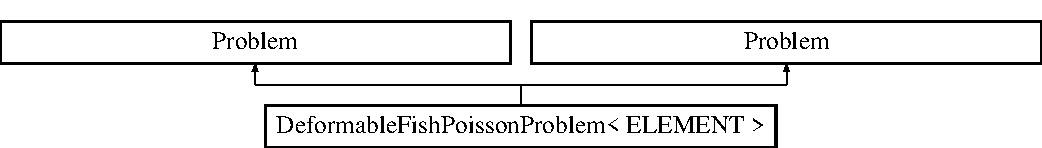
\includegraphics[height=1.992882cm]{classDeformableFishPoissonProblem}
\end{center}
\end{figure}
\subsection*{Public Member Functions}
\begin{DoxyCompactItemize}
\item 
\hyperlink{classDeformableFishPoissonProblem_a383952a668f3cec16b85c6b35f437ddd}{Deformable\+Fish\+Poisson\+Problem} ()
\begin{DoxyCompactList}\small\item\em Constructor\+: \end{DoxyCompactList}\item 
void \hyperlink{classDeformableFishPoissonProblem_a0ef0e4ab464ab41a6f0b7e8a74a9c8a5}{run} ()
\begin{DoxyCompactList}\small\item\em Run simulation. \end{DoxyCompactList}\item 
\hyperlink{classElasticFishMesh}{Elastic\+Fish\+Mesh}$<$ E\+L\+E\+M\+E\+NT $>$ $\ast$ \hyperlink{classDeformableFishPoissonProblem_a5d392625fca2a9d2848205d1e0d016a8}{mesh\+\_\+pt} ()
\begin{DoxyCompactList}\small\item\em Access function for the specific mesh. \end{DoxyCompactList}\item 
void \hyperlink{classDeformableFishPoissonProblem_aee9b59f35d1ae98cda29fba0c01b226a}{doc\+\_\+solution} (Doc\+Info \&doc\+\_\+info)
\begin{DoxyCompactList}\small\item\em Doc the solution. \end{DoxyCompactList}\item 
void \hyperlink{classDeformableFishPoissonProblem_a18fdfaadd9ae10257088b9533f139182}{actions\+\_\+after\+\_\+newton\+\_\+solve} ()
\begin{DoxyCompactList}\small\item\em Update function (empty) \end{DoxyCompactList}\item 
void \hyperlink{classDeformableFishPoissonProblem_ad9d03c8349a059430f7329354033b450}{actions\+\_\+before\+\_\+newton\+\_\+solve} ()
\begin{DoxyCompactList}\small\item\em Update before solve\+: We\textquotesingle{}re dealing with a static problem so the nodal positions before the next solve merely serve as initial conditions. For meshes that are very strongly refined near the boundary, the update of the displacement boundary conditions (which only moves the Solid\+Nodes {\itshape on} the boundary), can lead to strongly distorted meshes. This can cause the Newton method to fail --$>$ the overall method is actually more robust if we use the nodal positions as determined by the Domain/\+Macro\+Element-\/ based mesh update as initial guesses. \end{DoxyCompactList}\item 
void \hyperlink{classDeformableFishPoissonProblem_ada340a31a3b019116ecb7c0bb1d4c779}{actions\+\_\+after\+\_\+adapt} ()
\begin{DoxyCompactList}\small\item\em Update after adapt\+: Pin all redundant solid pressure nodes (if required) \end{DoxyCompactList}\item 
\hyperlink{classDeformableFishPoissonProblem_a383952a668f3cec16b85c6b35f437ddd}{Deformable\+Fish\+Poisson\+Problem} ()
\begin{DoxyCompactList}\small\item\em Constructor\+: \end{DoxyCompactList}\item 
void \hyperlink{classDeformableFishPoissonProblem_a0ef0e4ab464ab41a6f0b7e8a74a9c8a5}{run} ()
\begin{DoxyCompactList}\small\item\em Run simulation. \end{DoxyCompactList}\item 
\hyperlink{classElasticFishMesh}{Elastic\+Fish\+Mesh}$<$ E\+L\+E\+M\+E\+NT $>$ $\ast$ \hyperlink{classDeformableFishPoissonProblem_a5d392625fca2a9d2848205d1e0d016a8}{mesh\+\_\+pt} ()
\begin{DoxyCompactList}\small\item\em Access function for the specific mesh. \end{DoxyCompactList}\item 
void \hyperlink{classDeformableFishPoissonProblem_aee9b59f35d1ae98cda29fba0c01b226a}{doc\+\_\+solution} (Doc\+Info \&doc\+\_\+info)
\begin{DoxyCompactList}\small\item\em Doc the solution. \end{DoxyCompactList}\item 
void \hyperlink{classDeformableFishPoissonProblem_a18fdfaadd9ae10257088b9533f139182}{actions\+\_\+after\+\_\+newton\+\_\+solve} ()
\begin{DoxyCompactList}\small\item\em Update function (empty) \end{DoxyCompactList}\item 
void \hyperlink{classDeformableFishPoissonProblem_ad9d03c8349a059430f7329354033b450}{actions\+\_\+before\+\_\+newton\+\_\+solve} ()
\begin{DoxyCompactList}\small\item\em Update before solve\+: We\textquotesingle{}re dealing with a static problem so the nodal positions before the next solve merely serve as initial conditions. For meshes that are very strongly refined near the boundary, the update of the displacement boundary conditions (which only moves the Solid\+Nodes {\itshape on} the boundary), can lead to strongly distorted meshes. This can cause the Newton method to fail --$>$ the overall method is actually more robust if we use the nodal positions as determined by the Domain/\+Macro\+Element-\/ based mesh update as initial guesses. \end{DoxyCompactList}\item 
void \hyperlink{classDeformableFishPoissonProblem_ada340a31a3b019116ecb7c0bb1d4c779}{actions\+\_\+after\+\_\+adapt} ()
\begin{DoxyCompactList}\small\item\em Update after adapt\+: Pin all redundant solid pressure nodes (if required) \end{DoxyCompactList}\end{DoxyCompactItemize}
\subsection*{Private Attributes}
\begin{DoxyCompactItemize}
\item 
Node $\ast$ \hyperlink{classDeformableFishPoissonProblem_acdb029d569c5ecefa5a71f2f099e7f27}{Doc\+\_\+node\+\_\+pt}
\begin{DoxyCompactList}\small\item\em Node at which the solution of the Poisson equation is documented. \end{DoxyCompactList}\item 
ofstream \hyperlink{classDeformableFishPoissonProblem_a9fc310452a96891d566f50f3a231d5d5}{Trace\+\_\+file}
\begin{DoxyCompactList}\small\item\em Trace file. \end{DoxyCompactList}\item 
Circle $\ast$ \hyperlink{classDeformableFishPoissonProblem_a88745d43dc7a9377c13190ce1bed79e7}{Fish\+\_\+back\+\_\+pt}
\item 
\hyperlink{classoomph_1_1ElasticallySupportedRingElement}{Elastically\+Supported\+Ring\+Element} $\ast$ \hyperlink{classDeformableFishPoissonProblem_aaf5e3c5b0fc0e299b56f3d10d6dcbe20}{Fish\+\_\+back\+\_\+pt}
\end{DoxyCompactItemize}


\subsection{Detailed Description}
\subsubsection*{template$<$class E\+L\+E\+M\+E\+NT$>$\newline
class Deformable\+Fish\+Poisson\+Problem$<$ E\+L\+E\+M\+E\+N\+T $>$}

Solve Poisson equation on deforming fish-\/shaped domain. Mesh update via pseudo-\/elasticity. 

Definition at line 181 of file elastic\+\_\+mesh\+\_\+update.\+cc.



\subsection{Constructor \& Destructor Documentation}
\mbox{\Hypertarget{classDeformableFishPoissonProblem_a383952a668f3cec16b85c6b35f437ddd}\label{classDeformableFishPoissonProblem_a383952a668f3cec16b85c6b35f437ddd}} 
\index{Deformable\+Fish\+Poisson\+Problem@{Deformable\+Fish\+Poisson\+Problem}!Deformable\+Fish\+Poisson\+Problem@{Deformable\+Fish\+Poisson\+Problem}}
\index{Deformable\+Fish\+Poisson\+Problem@{Deformable\+Fish\+Poisson\+Problem}!Deformable\+Fish\+Poisson\+Problem@{Deformable\+Fish\+Poisson\+Problem}}
\subsubsection{\texorpdfstring{Deformable\+Fish\+Poisson\+Problem()}{DeformableFishPoissonProblem()}\hspace{0.1cm}{\footnotesize\ttfamily [1/2]}}
{\footnotesize\ttfamily template$<$class E\+L\+E\+M\+E\+NT $>$ \\
\hyperlink{classDeformableFishPoissonProblem}{Deformable\+Fish\+Poisson\+Problem}$<$ E\+L\+E\+M\+E\+NT $>$\+::\hyperlink{classDeformableFishPoissonProblem}{Deformable\+Fish\+Poisson\+Problem} (\begin{DoxyParamCaption}{ }\end{DoxyParamCaption})}



Constructor\+: 

Loop over elements and set pointers to source function 

Definition at line 247 of file elastic\+\_\+mesh\+\_\+update.\+cc.



References Global\+\_\+\+Physical\+\_\+\+Variables\+::\+Constitutive\+\_\+law\+\_\+pt, and Const\+Source\+For\+Poisson\+::get\+\_\+source().

\mbox{\Hypertarget{classDeformableFishPoissonProblem_a383952a668f3cec16b85c6b35f437ddd}\label{classDeformableFishPoissonProblem_a383952a668f3cec16b85c6b35f437ddd}} 
\index{Deformable\+Fish\+Poisson\+Problem@{Deformable\+Fish\+Poisson\+Problem}!Deformable\+Fish\+Poisson\+Problem@{Deformable\+Fish\+Poisson\+Problem}}
\index{Deformable\+Fish\+Poisson\+Problem@{Deformable\+Fish\+Poisson\+Problem}!Deformable\+Fish\+Poisson\+Problem@{Deformable\+Fish\+Poisson\+Problem}}
\subsubsection{\texorpdfstring{Deformable\+Fish\+Poisson\+Problem()}{DeformableFishPoissonProblem()}\hspace{0.1cm}{\footnotesize\ttfamily [2/2]}}
{\footnotesize\ttfamily template$<$class E\+L\+E\+M\+E\+NT $>$ \\
\hyperlink{classDeformableFishPoissonProblem}{Deformable\+Fish\+Poisson\+Problem}$<$ E\+L\+E\+M\+E\+NT $>$\+::\hyperlink{classDeformableFishPoissonProblem}{Deformable\+Fish\+Poisson\+Problem} (\begin{DoxyParamCaption}{ }\end{DoxyParamCaption})}



Constructor\+: 



\subsection{Member Function Documentation}
\mbox{\Hypertarget{classDeformableFishPoissonProblem_ada340a31a3b019116ecb7c0bb1d4c779}\label{classDeformableFishPoissonProblem_ada340a31a3b019116ecb7c0bb1d4c779}} 
\index{Deformable\+Fish\+Poisson\+Problem@{Deformable\+Fish\+Poisson\+Problem}!actions\+\_\+after\+\_\+adapt@{actions\+\_\+after\+\_\+adapt}}
\index{actions\+\_\+after\+\_\+adapt@{actions\+\_\+after\+\_\+adapt}!Deformable\+Fish\+Poisson\+Problem@{Deformable\+Fish\+Poisson\+Problem}}
\subsubsection{\texorpdfstring{actions\+\_\+after\+\_\+adapt()}{actions\_after\_adapt()}\hspace{0.1cm}{\footnotesize\ttfamily [1/2]}}
{\footnotesize\ttfamily template$<$class E\+L\+E\+M\+E\+NT $>$ \\
void \hyperlink{classDeformableFishPoissonProblem}{Deformable\+Fish\+Poisson\+Problem}$<$ E\+L\+E\+M\+E\+NT $>$\+::actions\+\_\+after\+\_\+adapt (\begin{DoxyParamCaption}{ }\end{DoxyParamCaption})\hspace{0.3cm}{\ttfamily [inline]}}



Update after adapt\+: Pin all redundant solid pressure nodes (if required) 



Definition at line 221 of file elastic\+\_\+poisson.\+cc.

\mbox{\Hypertarget{classDeformableFishPoissonProblem_ada340a31a3b019116ecb7c0bb1d4c779}\label{classDeformableFishPoissonProblem_ada340a31a3b019116ecb7c0bb1d4c779}} 
\index{Deformable\+Fish\+Poisson\+Problem@{Deformable\+Fish\+Poisson\+Problem}!actions\+\_\+after\+\_\+adapt@{actions\+\_\+after\+\_\+adapt}}
\index{actions\+\_\+after\+\_\+adapt@{actions\+\_\+after\+\_\+adapt}!Deformable\+Fish\+Poisson\+Problem@{Deformable\+Fish\+Poisson\+Problem}}
\subsubsection{\texorpdfstring{actions\+\_\+after\+\_\+adapt()}{actions\_after\_adapt()}\hspace{0.1cm}{\footnotesize\ttfamily [2/2]}}
{\footnotesize\ttfamily template$<$class E\+L\+E\+M\+E\+NT $>$ \\
void \hyperlink{classDeformableFishPoissonProblem}{Deformable\+Fish\+Poisson\+Problem}$<$ E\+L\+E\+M\+E\+NT $>$\+::actions\+\_\+after\+\_\+adapt (\begin{DoxyParamCaption}{ }\end{DoxyParamCaption})\hspace{0.3cm}{\ttfamily [inline]}}



Update after adapt\+: Pin all redundant solid pressure nodes (if required) 



Definition at line 222 of file elastic\+\_\+mesh\+\_\+update.\+cc.

\mbox{\Hypertarget{classDeformableFishPoissonProblem_a18fdfaadd9ae10257088b9533f139182}\label{classDeformableFishPoissonProblem_a18fdfaadd9ae10257088b9533f139182}} 
\index{Deformable\+Fish\+Poisson\+Problem@{Deformable\+Fish\+Poisson\+Problem}!actions\+\_\+after\+\_\+newton\+\_\+solve@{actions\+\_\+after\+\_\+newton\+\_\+solve}}
\index{actions\+\_\+after\+\_\+newton\+\_\+solve@{actions\+\_\+after\+\_\+newton\+\_\+solve}!Deformable\+Fish\+Poisson\+Problem@{Deformable\+Fish\+Poisson\+Problem}}
\subsubsection{\texorpdfstring{actions\+\_\+after\+\_\+newton\+\_\+solve()}{actions\_after\_newton\_solve()}\hspace{0.1cm}{\footnotesize\ttfamily [1/2]}}
{\footnotesize\ttfamily template$<$class E\+L\+E\+M\+E\+NT $>$ \\
void \hyperlink{classDeformableFishPoissonProblem}{Deformable\+Fish\+Poisson\+Problem}$<$ E\+L\+E\+M\+E\+NT $>$\+::actions\+\_\+after\+\_\+newton\+\_\+solve (\begin{DoxyParamCaption}{ }\end{DoxyParamCaption})\hspace{0.3cm}{\ttfamily [inline]}}



Update function (empty) 



Definition at line 200 of file elastic\+\_\+mesh\+\_\+update.\+cc.

\mbox{\Hypertarget{classDeformableFishPoissonProblem_a18fdfaadd9ae10257088b9533f139182}\label{classDeformableFishPoissonProblem_a18fdfaadd9ae10257088b9533f139182}} 
\index{Deformable\+Fish\+Poisson\+Problem@{Deformable\+Fish\+Poisson\+Problem}!actions\+\_\+after\+\_\+newton\+\_\+solve@{actions\+\_\+after\+\_\+newton\+\_\+solve}}
\index{actions\+\_\+after\+\_\+newton\+\_\+solve@{actions\+\_\+after\+\_\+newton\+\_\+solve}!Deformable\+Fish\+Poisson\+Problem@{Deformable\+Fish\+Poisson\+Problem}}
\subsubsection{\texorpdfstring{actions\+\_\+after\+\_\+newton\+\_\+solve()}{actions\_after\_newton\_solve()}\hspace{0.1cm}{\footnotesize\ttfamily [2/2]}}
{\footnotesize\ttfamily template$<$class E\+L\+E\+M\+E\+NT $>$ \\
void \hyperlink{classDeformableFishPoissonProblem}{Deformable\+Fish\+Poisson\+Problem}$<$ E\+L\+E\+M\+E\+NT $>$\+::actions\+\_\+after\+\_\+newton\+\_\+solve (\begin{DoxyParamCaption}{ }\end{DoxyParamCaption})\hspace{0.3cm}{\ttfamily [inline]}}



Update function (empty) 



Definition at line 203 of file elastic\+\_\+poisson.\+cc.

\mbox{\Hypertarget{classDeformableFishPoissonProblem_ad9d03c8349a059430f7329354033b450}\label{classDeformableFishPoissonProblem_ad9d03c8349a059430f7329354033b450}} 
\index{Deformable\+Fish\+Poisson\+Problem@{Deformable\+Fish\+Poisson\+Problem}!actions\+\_\+before\+\_\+newton\+\_\+solve@{actions\+\_\+before\+\_\+newton\+\_\+solve}}
\index{actions\+\_\+before\+\_\+newton\+\_\+solve@{actions\+\_\+before\+\_\+newton\+\_\+solve}!Deformable\+Fish\+Poisson\+Problem@{Deformable\+Fish\+Poisson\+Problem}}
\subsubsection{\texorpdfstring{actions\+\_\+before\+\_\+newton\+\_\+solve()}{actions\_before\_newton\_solve()}\hspace{0.1cm}{\footnotesize\ttfamily [1/2]}}
{\footnotesize\ttfamily template$<$class E\+L\+E\+M\+E\+NT $>$ \\
void \hyperlink{classDeformableFishPoissonProblem}{Deformable\+Fish\+Poisson\+Problem}$<$ E\+L\+E\+M\+E\+NT $>$\+::actions\+\_\+before\+\_\+newton\+\_\+solve (\begin{DoxyParamCaption}{ }\end{DoxyParamCaption})\hspace{0.3cm}{\ttfamily [inline]}}



Update before solve\+: We\textquotesingle{}re dealing with a static problem so the nodal positions before the next solve merely serve as initial conditions. For meshes that are very strongly refined near the boundary, the update of the displacement boundary conditions (which only moves the Solid\+Nodes {\itshape on} the boundary), can lead to strongly distorted meshes. This can cause the Newton method to fail --$>$ the overall method is actually more robust if we use the nodal positions as determined by the Domain/\+Macro\+Element-\/ based mesh update as initial guesses. 



Definition at line 211 of file elastic\+\_\+mesh\+\_\+update.\+cc.

\mbox{\Hypertarget{classDeformableFishPoissonProblem_ad9d03c8349a059430f7329354033b450}\label{classDeformableFishPoissonProblem_ad9d03c8349a059430f7329354033b450}} 
\index{Deformable\+Fish\+Poisson\+Problem@{Deformable\+Fish\+Poisson\+Problem}!actions\+\_\+before\+\_\+newton\+\_\+solve@{actions\+\_\+before\+\_\+newton\+\_\+solve}}
\index{actions\+\_\+before\+\_\+newton\+\_\+solve@{actions\+\_\+before\+\_\+newton\+\_\+solve}!Deformable\+Fish\+Poisson\+Problem@{Deformable\+Fish\+Poisson\+Problem}}
\subsubsection{\texorpdfstring{actions\+\_\+before\+\_\+newton\+\_\+solve()}{actions\_before\_newton\_solve()}\hspace{0.1cm}{\footnotesize\ttfamily [2/2]}}
{\footnotesize\ttfamily template$<$class E\+L\+E\+M\+E\+NT $>$ \\
void \hyperlink{classDeformableFishPoissonProblem}{Deformable\+Fish\+Poisson\+Problem}$<$ E\+L\+E\+M\+E\+NT $>$\+::actions\+\_\+before\+\_\+newton\+\_\+solve (\begin{DoxyParamCaption}{ }\end{DoxyParamCaption})\hspace{0.3cm}{\ttfamily [inline]}}



Update before solve\+: We\textquotesingle{}re dealing with a static problem so the nodal positions before the next solve merely serve as initial conditions. For meshes that are very strongly refined near the boundary, the update of the displacement boundary conditions (which only moves the Solid\+Nodes {\itshape on} the boundary), can lead to strongly distorted meshes. This can cause the Newton method to fail --$>$ the overall method is actually more robust if we use the nodal positions as determined by the Domain/\+Macro\+Element-\/ based mesh update as initial guesses. 



Definition at line 214 of file elastic\+\_\+poisson.\+cc.

\mbox{\Hypertarget{classDeformableFishPoissonProblem_aee9b59f35d1ae98cda29fba0c01b226a}\label{classDeformableFishPoissonProblem_aee9b59f35d1ae98cda29fba0c01b226a}} 
\index{Deformable\+Fish\+Poisson\+Problem@{Deformable\+Fish\+Poisson\+Problem}!doc\+\_\+solution@{doc\+\_\+solution}}
\index{doc\+\_\+solution@{doc\+\_\+solution}!Deformable\+Fish\+Poisson\+Problem@{Deformable\+Fish\+Poisson\+Problem}}
\subsubsection{\texorpdfstring{doc\+\_\+solution()}{doc\_solution()}\hspace{0.1cm}{\footnotesize\ttfamily [1/2]}}
{\footnotesize\ttfamily template$<$class E\+L\+E\+M\+E\+NT $>$ \\
void \hyperlink{classDeformableFishPoissonProblem}{Deformable\+Fish\+Poisson\+Problem}$<$ E\+L\+E\+M\+E\+NT $>$\+::doc\+\_\+solution (\begin{DoxyParamCaption}\item[{Doc\+Info \&}]{doc\+\_\+info }\end{DoxyParamCaption})}



Doc the solution. 



Definition at line 392 of file elastic\+\_\+mesh\+\_\+update.\+cc.

\mbox{\Hypertarget{classDeformableFishPoissonProblem_aee9b59f35d1ae98cda29fba0c01b226a}\label{classDeformableFishPoissonProblem_aee9b59f35d1ae98cda29fba0c01b226a}} 
\index{Deformable\+Fish\+Poisson\+Problem@{Deformable\+Fish\+Poisson\+Problem}!doc\+\_\+solution@{doc\+\_\+solution}}
\index{doc\+\_\+solution@{doc\+\_\+solution}!Deformable\+Fish\+Poisson\+Problem@{Deformable\+Fish\+Poisson\+Problem}}
\subsubsection{\texorpdfstring{doc\+\_\+solution()}{doc\_solution()}\hspace{0.1cm}{\footnotesize\ttfamily [2/2]}}
{\footnotesize\ttfamily template$<$class E\+L\+E\+M\+E\+NT $>$ \\
void \hyperlink{classDeformableFishPoissonProblem}{Deformable\+Fish\+Poisson\+Problem}$<$ E\+L\+E\+M\+E\+NT $>$\+::doc\+\_\+solution (\begin{DoxyParamCaption}\item[{Doc\+Info \&}]{doc\+\_\+info }\end{DoxyParamCaption})}



Doc the solution. 

\mbox{\Hypertarget{classDeformableFishPoissonProblem_a5d392625fca2a9d2848205d1e0d016a8}\label{classDeformableFishPoissonProblem_a5d392625fca2a9d2848205d1e0d016a8}} 
\index{Deformable\+Fish\+Poisson\+Problem@{Deformable\+Fish\+Poisson\+Problem}!mesh\+\_\+pt@{mesh\+\_\+pt}}
\index{mesh\+\_\+pt@{mesh\+\_\+pt}!Deformable\+Fish\+Poisson\+Problem@{Deformable\+Fish\+Poisson\+Problem}}
\subsubsection{\texorpdfstring{mesh\+\_\+pt()}{mesh\_pt()}\hspace{0.1cm}{\footnotesize\ttfamily [1/2]}}
{\footnotesize\ttfamily template$<$class E\+L\+E\+M\+E\+NT $>$ \\
\hyperlink{classElasticFishMesh}{Elastic\+Fish\+Mesh}$<$E\+L\+E\+M\+E\+NT$>$$\ast$ \hyperlink{classDeformableFishPoissonProblem}{Deformable\+Fish\+Poisson\+Problem}$<$ E\+L\+E\+M\+E\+NT $>$\+::mesh\+\_\+pt (\begin{DoxyParamCaption}{ }\end{DoxyParamCaption})\hspace{0.3cm}{\ttfamily [inline]}}



Access function for the specific mesh. 



Definition at line 193 of file elastic\+\_\+mesh\+\_\+update.\+cc.

\mbox{\Hypertarget{classDeformableFishPoissonProblem_a5d392625fca2a9d2848205d1e0d016a8}\label{classDeformableFishPoissonProblem_a5d392625fca2a9d2848205d1e0d016a8}} 
\index{Deformable\+Fish\+Poisson\+Problem@{Deformable\+Fish\+Poisson\+Problem}!mesh\+\_\+pt@{mesh\+\_\+pt}}
\index{mesh\+\_\+pt@{mesh\+\_\+pt}!Deformable\+Fish\+Poisson\+Problem@{Deformable\+Fish\+Poisson\+Problem}}
\subsubsection{\texorpdfstring{mesh\+\_\+pt()}{mesh\_pt()}\hspace{0.1cm}{\footnotesize\ttfamily [2/2]}}
{\footnotesize\ttfamily template$<$class E\+L\+E\+M\+E\+NT $>$ \\
\hyperlink{classElasticFishMesh}{Elastic\+Fish\+Mesh}$<$E\+L\+E\+M\+E\+NT$>$$\ast$ \hyperlink{classDeformableFishPoissonProblem}{Deformable\+Fish\+Poisson\+Problem}$<$ E\+L\+E\+M\+E\+NT $>$\+::mesh\+\_\+pt (\begin{DoxyParamCaption}{ }\end{DoxyParamCaption})\hspace{0.3cm}{\ttfamily [inline]}}



Access function for the specific mesh. 



Definition at line 196 of file elastic\+\_\+poisson.\+cc.

\mbox{\Hypertarget{classDeformableFishPoissonProblem_a0ef0e4ab464ab41a6f0b7e8a74a9c8a5}\label{classDeformableFishPoissonProblem_a0ef0e4ab464ab41a6f0b7e8a74a9c8a5}} 
\index{Deformable\+Fish\+Poisson\+Problem@{Deformable\+Fish\+Poisson\+Problem}!run@{run}}
\index{run@{run}!Deformable\+Fish\+Poisson\+Problem@{Deformable\+Fish\+Poisson\+Problem}}
\subsubsection{\texorpdfstring{run()}{run()}\hspace{0.1cm}{\footnotesize\ttfamily [1/2]}}
{\footnotesize\ttfamily template$<$class E\+L\+E\+M\+E\+NT $>$ \\
void \hyperlink{classDeformableFishPoissonProblem}{Deformable\+Fish\+Poisson\+Problem}$<$ E\+L\+E\+M\+E\+NT $>$\+::run (\begin{DoxyParamCaption}{ }\end{DoxyParamCaption})}



Run simulation. 

Run the problem. 

Definition at line 421 of file elastic\+\_\+mesh\+\_\+update.\+cc.



Referenced by main().

\mbox{\Hypertarget{classDeformableFishPoissonProblem_a0ef0e4ab464ab41a6f0b7e8a74a9c8a5}\label{classDeformableFishPoissonProblem_a0ef0e4ab464ab41a6f0b7e8a74a9c8a5}} 
\index{Deformable\+Fish\+Poisson\+Problem@{Deformable\+Fish\+Poisson\+Problem}!run@{run}}
\index{run@{run}!Deformable\+Fish\+Poisson\+Problem@{Deformable\+Fish\+Poisson\+Problem}}
\subsubsection{\texorpdfstring{run()}{run()}\hspace{0.1cm}{\footnotesize\ttfamily [2/2]}}
{\footnotesize\ttfamily template$<$class E\+L\+E\+M\+E\+NT $>$ \\
void \hyperlink{classDeformableFishPoissonProblem}{Deformable\+Fish\+Poisson\+Problem}$<$ E\+L\+E\+M\+E\+NT $>$\+::run (\begin{DoxyParamCaption}{ }\end{DoxyParamCaption})}



Run simulation. 



\subsection{Member Data Documentation}
\mbox{\Hypertarget{classDeformableFishPoissonProblem_acdb029d569c5ecefa5a71f2f099e7f27}\label{classDeformableFishPoissonProblem_acdb029d569c5ecefa5a71f2f099e7f27}} 
\index{Deformable\+Fish\+Poisson\+Problem@{Deformable\+Fish\+Poisson\+Problem}!Doc\+\_\+node\+\_\+pt@{Doc\+\_\+node\+\_\+pt}}
\index{Doc\+\_\+node\+\_\+pt@{Doc\+\_\+node\+\_\+pt}!Deformable\+Fish\+Poisson\+Problem@{Deformable\+Fish\+Poisson\+Problem}}
\subsubsection{\texorpdfstring{Doc\+\_\+node\+\_\+pt}{Doc\_node\_pt}}
{\footnotesize\ttfamily template$<$class E\+L\+E\+M\+E\+NT $>$ \\
Node $\ast$ \hyperlink{classDeformableFishPoissonProblem}{Deformable\+Fish\+Poisson\+Problem}$<$ E\+L\+E\+M\+E\+NT $>$\+::Doc\+\_\+node\+\_\+pt\hspace{0.3cm}{\ttfamily [private]}}



Node at which the solution of the Poisson equation is documented. 



Definition at line 233 of file elastic\+\_\+mesh\+\_\+update.\+cc.

\mbox{\Hypertarget{classDeformableFishPoissonProblem_aaf5e3c5b0fc0e299b56f3d10d6dcbe20}\label{classDeformableFishPoissonProblem_aaf5e3c5b0fc0e299b56f3d10d6dcbe20}} 
\index{Deformable\+Fish\+Poisson\+Problem@{Deformable\+Fish\+Poisson\+Problem}!Fish\+\_\+back\+\_\+pt@{Fish\+\_\+back\+\_\+pt}}
\index{Fish\+\_\+back\+\_\+pt@{Fish\+\_\+back\+\_\+pt}!Deformable\+Fish\+Poisson\+Problem@{Deformable\+Fish\+Poisson\+Problem}}
\subsubsection{\texorpdfstring{Fish\+\_\+back\+\_\+pt}{Fish\_back\_pt}\hspace{0.1cm}{\footnotesize\ttfamily [1/2]}}
{\footnotesize\ttfamily template$<$class E\+L\+E\+M\+E\+NT $>$ \\
\hyperlink{classoomph_1_1ElasticallySupportedRingElement}{Elastically\+Supported\+Ring\+Element}$\ast$ \hyperlink{classDeformableFishPoissonProblem}{Deformable\+Fish\+Poisson\+Problem}$<$ E\+L\+E\+M\+E\+NT $>$\+::Fish\+\_\+back\+\_\+pt\hspace{0.3cm}{\ttfamily [private]}}



Definition at line 239 of file elastic\+\_\+poisson.\+cc.

\mbox{\Hypertarget{classDeformableFishPoissonProblem_a88745d43dc7a9377c13190ce1bed79e7}\label{classDeformableFishPoissonProblem_a88745d43dc7a9377c13190ce1bed79e7}} 
\index{Deformable\+Fish\+Poisson\+Problem@{Deformable\+Fish\+Poisson\+Problem}!Fish\+\_\+back\+\_\+pt@{Fish\+\_\+back\+\_\+pt}}
\index{Fish\+\_\+back\+\_\+pt@{Fish\+\_\+back\+\_\+pt}!Deformable\+Fish\+Poisson\+Problem@{Deformable\+Fish\+Poisson\+Problem}}
\subsubsection{\texorpdfstring{Fish\+\_\+back\+\_\+pt}{Fish\_back\_pt}\hspace{0.1cm}{\footnotesize\ttfamily [2/2]}}
{\footnotesize\ttfamily template$<$class E\+L\+E\+M\+E\+NT $>$ \\
Circle$\ast$ \hyperlink{classDeformableFishPoissonProblem}{Deformable\+Fish\+Poisson\+Problem}$<$ E\+L\+E\+M\+E\+NT $>$\+::Fish\+\_\+back\+\_\+pt\hspace{0.3cm}{\ttfamily [private]}}



Definition at line 239 of file elastic\+\_\+mesh\+\_\+update.\+cc.

\mbox{\Hypertarget{classDeformableFishPoissonProblem_a9fc310452a96891d566f50f3a231d5d5}\label{classDeformableFishPoissonProblem_a9fc310452a96891d566f50f3a231d5d5}} 
\index{Deformable\+Fish\+Poisson\+Problem@{Deformable\+Fish\+Poisson\+Problem}!Trace\+\_\+file@{Trace\+\_\+file}}
\index{Trace\+\_\+file@{Trace\+\_\+file}!Deformable\+Fish\+Poisson\+Problem@{Deformable\+Fish\+Poisson\+Problem}}
\subsubsection{\texorpdfstring{Trace\+\_\+file}{Trace\_file}}
{\footnotesize\ttfamily template$<$class E\+L\+E\+M\+E\+NT $>$ \\
ofstream \hyperlink{classDeformableFishPoissonProblem}{Deformable\+Fish\+Poisson\+Problem}$<$ E\+L\+E\+M\+E\+NT $>$\+::Trace\+\_\+file\hspace{0.3cm}{\ttfamily [private]}}



Trace file. 



Definition at line 236 of file elastic\+\_\+mesh\+\_\+update.\+cc.



The documentation for this class was generated from the following files\+:\begin{DoxyCompactItemize}
\item 
\hyperlink{elastic__mesh__update_8cc}{elastic\+\_\+mesh\+\_\+update.\+cc}\item 
\hyperlink{elastic__poisson_8cc}{elastic\+\_\+poisson.\+cc}\end{DoxyCompactItemize}

\hypertarget{classoomph_1_1ElasticallySupportedRingElement}{}\section{oomph\+:\+:Elastically\+Supported\+Ring\+Element Class Reference}
\label{classoomph_1_1ElasticallySupportedRingElement}\index{oomph\+::\+Elastically\+Supported\+Ring\+Element@{oomph\+::\+Elastically\+Supported\+Ring\+Element}}


\hyperlink{classoomph_1_1GeneralCircle}{General\+Circle} \char`\"{}upgraded\char`\"{} to a Generalised\+Element\+: Circular ring whose position is given by \[ x = X_c + R \cos(\zeta) \] \[ y = Y_c + R \sin(\zeta) \] The ring\textquotesingle{}s vertical position $ Y_c $ is determined by \char`\"{}pseudo elasticity\char`\"{}\+: \[ 0 = f_{load} - Y_c \ k_{stiff} \] This simulates the case where the centre of the ring is mounted on an elastic spring of stiffness $ k_{stiff} $ and loaded by the force $ f_{load}. $ The \char`\"{}load\char`\"{} is specified by the Data object {\ttfamily load\+\_\+pt()}.  




{\ttfamily \#include $<$circle\+\_\+as\+\_\+generalised\+\_\+element.\+h$>$}

Inheritance diagram for oomph\+:\+:Elastically\+Supported\+Ring\+Element\+:\begin{figure}[H]
\begin{center}
\leavevmode
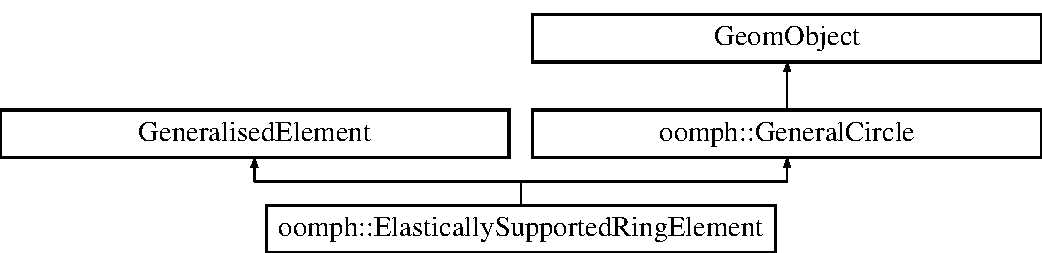
\includegraphics[height=3.000000cm]{classoomph_1_1ElasticallySupportedRingElement}
\end{center}
\end{figure}
\subsection*{Public Member Functions}
\begin{DoxyCompactItemize}
\item 
\hyperlink{classoomph_1_1ElasticallySupportedRingElement_a7e68f18d76acb6297405ca2a38b64898}{Elastically\+Supported\+Ring\+Element} (const double \&\hyperlink{classoomph_1_1GeneralCircle_a9c84564d8239bd8b4a2b28649638dd4a}{x\+\_\+c}, const double \&\hyperlink{classoomph_1_1GeneralCircle_afa91b6356920d73e05f81d6e7aaf0bf7}{y\+\_\+c}, const double \&r)
\begin{DoxyCompactList}\small\item\em Constructor\+: Build ring from doubles that describe the geometry\+: x and y positions of centre and the radius. Initialise stiffness to 1.\+0. By default, no load is set. \end{DoxyCompactList}\item 
virtual \hyperlink{classoomph_1_1ElasticallySupportedRingElement_a2b3fd2a41155a9d34ab0f43aa8a5deab}{$\sim$\+Elastically\+Supported\+Ring\+Element} ()
\begin{DoxyCompactList}\small\item\em Destructor\+: \end{DoxyCompactList}\item 
void \hyperlink{classoomph_1_1ElasticallySupportedRingElement_ac1c967080f2a4e6143bcffdcdbc1d735}{set\+\_\+load\+\_\+pt} (Data $\ast$load\+\_\+pt)
\begin{DoxyCompactList}\small\item\em Set pointer to Data object that specifies the \char`\"{}load\char`\"{} on the \hyperlink{classoomph_1_1ElasticallySupportedRingElement}{Elastically\+Supported\+Ring\+Element}. \end{DoxyCompactList}\item 
double \hyperlink{classoomph_1_1ElasticallySupportedRingElement_a636b98cd51286298efff1e89cd2c1c4f}{load} ()
\begin{DoxyCompactList}\small\item\em \char`\"{}\+Load\char`\"{} acting on the ring \end{DoxyCompactList}\item 
double \& \hyperlink{classoomph_1_1ElasticallySupportedRingElement_a660b5abfdc353e41848d00617b6ba434}{k\+\_\+stiff} ()
\begin{DoxyCompactList}\small\item\em Access function for the spring stiffness. \end{DoxyCompactList}\item 
void \hyperlink{classoomph_1_1ElasticallySupportedRingElement_acddd4ff64f173aa2d6c4e651c1c9c319}{pin\+\_\+yc} ()
\begin{DoxyCompactList}\small\item\em Pin the vertical displacement. \end{DoxyCompactList}\item 
void \hyperlink{classoomph_1_1ElasticallySupportedRingElement_ad70712dca329430d09d1a905c1362478}{unpin\+\_\+yc} ()
\begin{DoxyCompactList}\small\item\em Unpin the vertical displacement. \end{DoxyCompactList}\item 
void \hyperlink{classoomph_1_1ElasticallySupportedRingElement_ad8bf518168d68e8b016e474e76037a49}{get\+\_\+residuals} (Vector$<$ double $>$ \&residuals)
\begin{DoxyCompactList}\small\item\em Compute element residual vector (wrapper) \end{DoxyCompactList}\item 
void \hyperlink{classoomph_1_1ElasticallySupportedRingElement_a2418f706f5b17a64a5b01b72ccb3b95d}{get\+\_\+jacobian} (Vector$<$ double $>$ \&residuals, Dense\+Matrix$<$ double $>$ \&jacobian)
\begin{DoxyCompactList}\small\item\em Compute element residual Vector and element Jacobian matrix (wrapper) \end{DoxyCompactList}\end{DoxyCompactItemize}
\subsection*{Protected Member Functions}
\begin{DoxyCompactItemize}
\item 
void \hyperlink{classoomph_1_1ElasticallySupportedRingElement_a6d763f2ce0c930e7a2201e995290f169}{fill\+\_\+in\+\_\+generic\+\_\+residual\+\_\+contribution} (Vector$<$ double $>$ \&residuals, Dense\+Matrix$<$ double $>$ \&jacobian, unsigned flag)
\begin{DoxyCompactList}\small\item\em Compute element residual Vector (only if flag=0) and also the element Jacobian matrix (if flag=1) \end{DoxyCompactList}\end{DoxyCompactItemize}
\subsection*{Private Attributes}
\begin{DoxyCompactItemize}
\item 
double \hyperlink{classoomph_1_1ElasticallySupportedRingElement_ab6036a4f4e1434a2d068f6584f7c46e6}{K\+\_\+stiff}
\begin{DoxyCompactList}\small\item\em Stiffness of the ring\textquotesingle{}s \char`\"{}elastic\char`\"{} support. \end{DoxyCompactList}\item 
unsigned \hyperlink{classoomph_1_1ElasticallySupportedRingElement_a800f0a57477dc63df13aaea5c99a5f30}{External\+\_\+load\+\_\+index}
\begin{DoxyCompactList}\small\item\em Index of the location of the load Data in the element\textquotesingle{}s array of external data. \end{DoxyCompactList}\item 
unsigned \hyperlink{classoomph_1_1ElasticallySupportedRingElement_a6804e3aa5b62db4848416b2b69e89fe7}{Internal\+\_\+geometric\+\_\+data\+\_\+index}
\begin{DoxyCompactList}\small\item\em Index of the location of the geometric Data in the element\textquotesingle{}s array of internal data. \end{DoxyCompactList}\item 
bool \hyperlink{classoomph_1_1ElasticallySupportedRingElement_a98151ae912af71c1a78ddae80c4fbb04}{Load\+\_\+data\+\_\+has\+\_\+been\+\_\+set}
\begin{DoxyCompactList}\small\item\em Flag to indicate that load data has been set. \end{DoxyCompactList}\end{DoxyCompactItemize}
\subsection*{Additional Inherited Members}


\subsection{Detailed Description}
\hyperlink{classoomph_1_1GeneralCircle}{General\+Circle} \char`\"{}upgraded\char`\"{} to a Generalised\+Element\+: Circular ring whose position is given by \[ x = X_c + R \cos(\zeta) \] \[ y = Y_c + R \sin(\zeta) \] The ring\textquotesingle{}s vertical position $ Y_c $ is determined by \char`\"{}pseudo elasticity\char`\"{}\+: \[ 0 = f_{load} - Y_c \ k_{stiff} \] This simulates the case where the centre of the ring is mounted on an elastic spring of stiffness $ k_{stiff} $ and loaded by the force $ f_{load}. $ The \char`\"{}load\char`\"{} is specified by the Data object {\ttfamily load\+\_\+pt()}. 

Definition at line 59 of file circle\+\_\+as\+\_\+generalised\+\_\+element.\+h.



\subsection{Constructor \& Destructor Documentation}
\mbox{\Hypertarget{classoomph_1_1ElasticallySupportedRingElement_a7e68f18d76acb6297405ca2a38b64898}\label{classoomph_1_1ElasticallySupportedRingElement_a7e68f18d76acb6297405ca2a38b64898}} 
\index{oomph\+::\+Elastically\+Supported\+Ring\+Element@{oomph\+::\+Elastically\+Supported\+Ring\+Element}!Elastically\+Supported\+Ring\+Element@{Elastically\+Supported\+Ring\+Element}}
\index{Elastically\+Supported\+Ring\+Element@{Elastically\+Supported\+Ring\+Element}!oomph\+::\+Elastically\+Supported\+Ring\+Element@{oomph\+::\+Elastically\+Supported\+Ring\+Element}}
\subsubsection{\texorpdfstring{Elastically\+Supported\+Ring\+Element()}{ElasticallySupportedRingElement()}}
{\footnotesize\ttfamily oomph\+::\+Elastically\+Supported\+Ring\+Element\+::\+Elastically\+Supported\+Ring\+Element (\begin{DoxyParamCaption}\item[{const double \&}]{x\+\_\+c,  }\item[{const double \&}]{y\+\_\+c,  }\item[{const double \&}]{r }\end{DoxyParamCaption})\hspace{0.3cm}{\ttfamily [inline]}}



Constructor\+: Build ring from doubles that describe the geometry\+: x and y positions of centre and the radius. Initialise stiffness to 1.\+0. By default, no load is set. 



Definition at line 68 of file circle\+\_\+as\+\_\+generalised\+\_\+element.\+h.



References oomph\+::\+General\+Circle\+::\+Geom\+\_\+data\+\_\+pt, Internal\+\_\+geometric\+\_\+data\+\_\+index, and oomph\+::\+General\+Circle\+::\+Must\+\_\+clean\+\_\+up.

\mbox{\Hypertarget{classoomph_1_1ElasticallySupportedRingElement_a2b3fd2a41155a9d34ab0f43aa8a5deab}\label{classoomph_1_1ElasticallySupportedRingElement_a2b3fd2a41155a9d34ab0f43aa8a5deab}} 
\index{oomph\+::\+Elastically\+Supported\+Ring\+Element@{oomph\+::\+Elastically\+Supported\+Ring\+Element}!````~Elastically\+Supported\+Ring\+Element@{$\sim$\+Elastically\+Supported\+Ring\+Element}}
\index{````~Elastically\+Supported\+Ring\+Element@{$\sim$\+Elastically\+Supported\+Ring\+Element}!oomph\+::\+Elastically\+Supported\+Ring\+Element@{oomph\+::\+Elastically\+Supported\+Ring\+Element}}
\subsubsection{\texorpdfstring{$\sim$\+Elastically\+Supported\+Ring\+Element()}{~ElasticallySupportedRingElement()}}
{\footnotesize\ttfamily virtual oomph\+::\+Elastically\+Supported\+Ring\+Element\+::$\sim$\+Elastically\+Supported\+Ring\+Element (\begin{DoxyParamCaption}{ }\end{DoxyParamCaption})\hspace{0.3cm}{\ttfamily [inline]}, {\ttfamily [virtual]}}



Destructor\+: 



Definition at line 92 of file circle\+\_\+as\+\_\+generalised\+\_\+element.\+h.



\subsection{Member Function Documentation}
\mbox{\Hypertarget{classoomph_1_1ElasticallySupportedRingElement_a6d763f2ce0c930e7a2201e995290f169}\label{classoomph_1_1ElasticallySupportedRingElement_a6d763f2ce0c930e7a2201e995290f169}} 
\index{oomph\+::\+Elastically\+Supported\+Ring\+Element@{oomph\+::\+Elastically\+Supported\+Ring\+Element}!fill\+\_\+in\+\_\+generic\+\_\+residual\+\_\+contribution@{fill\+\_\+in\+\_\+generic\+\_\+residual\+\_\+contribution}}
\index{fill\+\_\+in\+\_\+generic\+\_\+residual\+\_\+contribution@{fill\+\_\+in\+\_\+generic\+\_\+residual\+\_\+contribution}!oomph\+::\+Elastically\+Supported\+Ring\+Element@{oomph\+::\+Elastically\+Supported\+Ring\+Element}}
\subsubsection{\texorpdfstring{fill\+\_\+in\+\_\+generic\+\_\+residual\+\_\+contribution()}{fill\_in\_generic\_residual\_contribution()}}
{\footnotesize\ttfamily void oomph\+::\+Elastically\+Supported\+Ring\+Element\+::fill\+\_\+in\+\_\+generic\+\_\+residual\+\_\+contribution (\begin{DoxyParamCaption}\item[{Vector$<$ double $>$ \&}]{residuals,  }\item[{Dense\+Matrix$<$ double $>$ \&}]{jacobian,  }\item[{unsigned}]{flag }\end{DoxyParamCaption})\hspace{0.3cm}{\ttfamily [inline]}, {\ttfamily [protected]}}



Compute element residual Vector (only if flag=0) and also the element Jacobian matrix (if flag=1) 



Definition at line 201 of file circle\+\_\+as\+\_\+generalised\+\_\+element.\+h.



References External\+\_\+load\+\_\+index, Internal\+\_\+geometric\+\_\+data\+\_\+index, K\+\_\+stiff, load(), and oomph\+::\+General\+Circle\+::y\+\_\+c().



Referenced by get\+\_\+jacobian(), and get\+\_\+residuals().

\mbox{\Hypertarget{classoomph_1_1ElasticallySupportedRingElement_a2418f706f5b17a64a5b01b72ccb3b95d}\label{classoomph_1_1ElasticallySupportedRingElement_a2418f706f5b17a64a5b01b72ccb3b95d}} 
\index{oomph\+::\+Elastically\+Supported\+Ring\+Element@{oomph\+::\+Elastically\+Supported\+Ring\+Element}!get\+\_\+jacobian@{get\+\_\+jacobian}}
\index{get\+\_\+jacobian@{get\+\_\+jacobian}!oomph\+::\+Elastically\+Supported\+Ring\+Element@{oomph\+::\+Elastically\+Supported\+Ring\+Element}}
\subsubsection{\texorpdfstring{get\+\_\+jacobian()}{get\_jacobian()}}
{\footnotesize\ttfamily void oomph\+::\+Elastically\+Supported\+Ring\+Element\+::get\+\_\+jacobian (\begin{DoxyParamCaption}\item[{Vector$<$ double $>$ \&}]{residuals,  }\item[{Dense\+Matrix$<$ double $>$ \&}]{jacobian }\end{DoxyParamCaption})\hspace{0.3cm}{\ttfamily [inline]}}



Compute element residual Vector and element Jacobian matrix (wrapper) 



Definition at line 183 of file circle\+\_\+as\+\_\+generalised\+\_\+element.\+h.



References fill\+\_\+in\+\_\+generic\+\_\+residual\+\_\+contribution().

\mbox{\Hypertarget{classoomph_1_1ElasticallySupportedRingElement_ad8bf518168d68e8b016e474e76037a49}\label{classoomph_1_1ElasticallySupportedRingElement_ad8bf518168d68e8b016e474e76037a49}} 
\index{oomph\+::\+Elastically\+Supported\+Ring\+Element@{oomph\+::\+Elastically\+Supported\+Ring\+Element}!get\+\_\+residuals@{get\+\_\+residuals}}
\index{get\+\_\+residuals@{get\+\_\+residuals}!oomph\+::\+Elastically\+Supported\+Ring\+Element@{oomph\+::\+Elastically\+Supported\+Ring\+Element}}
\subsubsection{\texorpdfstring{get\+\_\+residuals()}{get\_residuals()}}
{\footnotesize\ttfamily void oomph\+::\+Elastically\+Supported\+Ring\+Element\+::get\+\_\+residuals (\begin{DoxyParamCaption}\item[{Vector$<$ double $>$ \&}]{residuals }\end{DoxyParamCaption})\hspace{0.3cm}{\ttfamily [inline]}}



Compute element residual vector (wrapper) 



Definition at line 171 of file circle\+\_\+as\+\_\+generalised\+\_\+element.\+h.



References fill\+\_\+in\+\_\+generic\+\_\+residual\+\_\+contribution().

\mbox{\Hypertarget{classoomph_1_1ElasticallySupportedRingElement_a660b5abfdc353e41848d00617b6ba434}\label{classoomph_1_1ElasticallySupportedRingElement_a660b5abfdc353e41848d00617b6ba434}} 
\index{oomph\+::\+Elastically\+Supported\+Ring\+Element@{oomph\+::\+Elastically\+Supported\+Ring\+Element}!k\+\_\+stiff@{k\+\_\+stiff}}
\index{k\+\_\+stiff@{k\+\_\+stiff}!oomph\+::\+Elastically\+Supported\+Ring\+Element@{oomph\+::\+Elastically\+Supported\+Ring\+Element}}
\subsubsection{\texorpdfstring{k\+\_\+stiff()}{k\_stiff()}}
{\footnotesize\ttfamily double\& oomph\+::\+Elastically\+Supported\+Ring\+Element\+::k\+\_\+stiff (\begin{DoxyParamCaption}{ }\end{DoxyParamCaption})\hspace{0.3cm}{\ttfamily [inline]}}



Access function for the spring stiffness. 



Definition at line 148 of file circle\+\_\+as\+\_\+generalised\+\_\+element.\+h.



References K\+\_\+stiff.



Referenced by Geom\+Object\+As\+Generalised\+Element\+Problem\+::\+Geom\+Object\+As\+Generalised\+Element\+Problem().

\mbox{\Hypertarget{classoomph_1_1ElasticallySupportedRingElement_a636b98cd51286298efff1e89cd2c1c4f}\label{classoomph_1_1ElasticallySupportedRingElement_a636b98cd51286298efff1e89cd2c1c4f}} 
\index{oomph\+::\+Elastically\+Supported\+Ring\+Element@{oomph\+::\+Elastically\+Supported\+Ring\+Element}!load@{load}}
\index{load@{load}!oomph\+::\+Elastically\+Supported\+Ring\+Element@{oomph\+::\+Elastically\+Supported\+Ring\+Element}}
\subsubsection{\texorpdfstring{load()}{load()}}
{\footnotesize\ttfamily double oomph\+::\+Elastically\+Supported\+Ring\+Element\+::load (\begin{DoxyParamCaption}{ }\end{DoxyParamCaption})\hspace{0.3cm}{\ttfamily [inline]}}



\char`\"{}\+Load\char`\"{} acting on the ring 



Definition at line 132 of file circle\+\_\+as\+\_\+generalised\+\_\+element.\+h.



References External\+\_\+load\+\_\+index, and Load\+\_\+data\+\_\+has\+\_\+been\+\_\+set.



Referenced by fill\+\_\+in\+\_\+generic\+\_\+residual\+\_\+contribution().

\mbox{\Hypertarget{classoomph_1_1ElasticallySupportedRingElement_acddd4ff64f173aa2d6c4e651c1c9c319}\label{classoomph_1_1ElasticallySupportedRingElement_acddd4ff64f173aa2d6c4e651c1c9c319}} 
\index{oomph\+::\+Elastically\+Supported\+Ring\+Element@{oomph\+::\+Elastically\+Supported\+Ring\+Element}!pin\+\_\+yc@{pin\+\_\+yc}}
\index{pin\+\_\+yc@{pin\+\_\+yc}!oomph\+::\+Elastically\+Supported\+Ring\+Element@{oomph\+::\+Elastically\+Supported\+Ring\+Element}}
\subsubsection{\texorpdfstring{pin\+\_\+yc()}{pin\_yc()}}
{\footnotesize\ttfamily void oomph\+::\+Elastically\+Supported\+Ring\+Element\+::pin\+\_\+yc (\begin{DoxyParamCaption}{ }\end{DoxyParamCaption})\hspace{0.3cm}{\ttfamily [inline]}}



Pin the vertical displacement. 



Definition at line 152 of file circle\+\_\+as\+\_\+generalised\+\_\+element.\+h.



References Internal\+\_\+geometric\+\_\+data\+\_\+index.

\mbox{\Hypertarget{classoomph_1_1ElasticallySupportedRingElement_ac1c967080f2a4e6143bcffdcdbc1d735}\label{classoomph_1_1ElasticallySupportedRingElement_ac1c967080f2a4e6143bcffdcdbc1d735}} 
\index{oomph\+::\+Elastically\+Supported\+Ring\+Element@{oomph\+::\+Elastically\+Supported\+Ring\+Element}!set\+\_\+load\+\_\+pt@{set\+\_\+load\+\_\+pt}}
\index{set\+\_\+load\+\_\+pt@{set\+\_\+load\+\_\+pt}!oomph\+::\+Elastically\+Supported\+Ring\+Element@{oomph\+::\+Elastically\+Supported\+Ring\+Element}}
\subsubsection{\texorpdfstring{set\+\_\+load\+\_\+pt()}{set\_load\_pt()}}
{\footnotesize\ttfamily void oomph\+::\+Elastically\+Supported\+Ring\+Element\+::set\+\_\+load\+\_\+pt (\begin{DoxyParamCaption}\item[{Data $\ast$}]{load\+\_\+pt }\end{DoxyParamCaption})\hspace{0.3cm}{\ttfamily [inline]}}



Set pointer to Data object that specifies the \char`\"{}load\char`\"{} on the \hyperlink{classoomph_1_1ElasticallySupportedRingElement}{Elastically\+Supported\+Ring\+Element}. 



Definition at line 102 of file circle\+\_\+as\+\_\+generalised\+\_\+element.\+h.



References External\+\_\+load\+\_\+index, and Load\+\_\+data\+\_\+has\+\_\+been\+\_\+set.



Referenced by Geom\+Object\+As\+Generalised\+Element\+Problem\+::\+Geom\+Object\+As\+Generalised\+Element\+Problem().

\mbox{\Hypertarget{classoomph_1_1ElasticallySupportedRingElement_ad70712dca329430d09d1a905c1362478}\label{classoomph_1_1ElasticallySupportedRingElement_ad70712dca329430d09d1a905c1362478}} 
\index{oomph\+::\+Elastically\+Supported\+Ring\+Element@{oomph\+::\+Elastically\+Supported\+Ring\+Element}!unpin\+\_\+yc@{unpin\+\_\+yc}}
\index{unpin\+\_\+yc@{unpin\+\_\+yc}!oomph\+::\+Elastically\+Supported\+Ring\+Element@{oomph\+::\+Elastically\+Supported\+Ring\+Element}}
\subsubsection{\texorpdfstring{unpin\+\_\+yc()}{unpin\_yc()}}
{\footnotesize\ttfamily void oomph\+::\+Elastically\+Supported\+Ring\+Element\+::unpin\+\_\+yc (\begin{DoxyParamCaption}{ }\end{DoxyParamCaption})\hspace{0.3cm}{\ttfamily [inline]}}



Unpin the vertical displacement. 



Definition at line 161 of file circle\+\_\+as\+\_\+generalised\+\_\+element.\+h.



References Internal\+\_\+geometric\+\_\+data\+\_\+index.



\subsection{Member Data Documentation}
\mbox{\Hypertarget{classoomph_1_1ElasticallySupportedRingElement_a800f0a57477dc63df13aaea5c99a5f30}\label{classoomph_1_1ElasticallySupportedRingElement_a800f0a57477dc63df13aaea5c99a5f30}} 
\index{oomph\+::\+Elastically\+Supported\+Ring\+Element@{oomph\+::\+Elastically\+Supported\+Ring\+Element}!External\+\_\+load\+\_\+index@{External\+\_\+load\+\_\+index}}
\index{External\+\_\+load\+\_\+index@{External\+\_\+load\+\_\+index}!oomph\+::\+Elastically\+Supported\+Ring\+Element@{oomph\+::\+Elastically\+Supported\+Ring\+Element}}
\subsubsection{\texorpdfstring{External\+\_\+load\+\_\+index}{External\_load\_index}}
{\footnotesize\ttfamily unsigned oomph\+::\+Elastically\+Supported\+Ring\+Element\+::\+External\+\_\+load\+\_\+index\hspace{0.3cm}{\ttfamily [private]}}



Index of the location of the load Data in the element\textquotesingle{}s array of external data. 



Definition at line 266 of file circle\+\_\+as\+\_\+generalised\+\_\+element.\+h.



Referenced by fill\+\_\+in\+\_\+generic\+\_\+residual\+\_\+contribution(), load(), and set\+\_\+load\+\_\+pt().

\mbox{\Hypertarget{classoomph_1_1ElasticallySupportedRingElement_a6804e3aa5b62db4848416b2b69e89fe7}\label{classoomph_1_1ElasticallySupportedRingElement_a6804e3aa5b62db4848416b2b69e89fe7}} 
\index{oomph\+::\+Elastically\+Supported\+Ring\+Element@{oomph\+::\+Elastically\+Supported\+Ring\+Element}!Internal\+\_\+geometric\+\_\+data\+\_\+index@{Internal\+\_\+geometric\+\_\+data\+\_\+index}}
\index{Internal\+\_\+geometric\+\_\+data\+\_\+index@{Internal\+\_\+geometric\+\_\+data\+\_\+index}!oomph\+::\+Elastically\+Supported\+Ring\+Element@{oomph\+::\+Elastically\+Supported\+Ring\+Element}}
\subsubsection{\texorpdfstring{Internal\+\_\+geometric\+\_\+data\+\_\+index}{Internal\_geometric\_data\_index}}
{\footnotesize\ttfamily unsigned oomph\+::\+Elastically\+Supported\+Ring\+Element\+::\+Internal\+\_\+geometric\+\_\+data\+\_\+index\hspace{0.3cm}{\ttfamily [private]}}



Index of the location of the geometric Data in the element\textquotesingle{}s array of internal data. 



Definition at line 270 of file circle\+\_\+as\+\_\+generalised\+\_\+element.\+h.



Referenced by Elastically\+Supported\+Ring\+Element(), fill\+\_\+in\+\_\+generic\+\_\+residual\+\_\+contribution(), pin\+\_\+yc(), and unpin\+\_\+yc().

\mbox{\Hypertarget{classoomph_1_1ElasticallySupportedRingElement_ab6036a4f4e1434a2d068f6584f7c46e6}\label{classoomph_1_1ElasticallySupportedRingElement_ab6036a4f4e1434a2d068f6584f7c46e6}} 
\index{oomph\+::\+Elastically\+Supported\+Ring\+Element@{oomph\+::\+Elastically\+Supported\+Ring\+Element}!K\+\_\+stiff@{K\+\_\+stiff}}
\index{K\+\_\+stiff@{K\+\_\+stiff}!oomph\+::\+Elastically\+Supported\+Ring\+Element@{oomph\+::\+Elastically\+Supported\+Ring\+Element}}
\subsubsection{\texorpdfstring{K\+\_\+stiff}{K\_stiff}}
{\footnotesize\ttfamily double oomph\+::\+Elastically\+Supported\+Ring\+Element\+::\+K\+\_\+stiff\hspace{0.3cm}{\ttfamily [private]}}



Stiffness of the ring\textquotesingle{}s \char`\"{}elastic\char`\"{} support. 



Definition at line 262 of file circle\+\_\+as\+\_\+generalised\+\_\+element.\+h.



Referenced by fill\+\_\+in\+\_\+generic\+\_\+residual\+\_\+contribution(), and k\+\_\+stiff().

\mbox{\Hypertarget{classoomph_1_1ElasticallySupportedRingElement_a98151ae912af71c1a78ddae80c4fbb04}\label{classoomph_1_1ElasticallySupportedRingElement_a98151ae912af71c1a78ddae80c4fbb04}} 
\index{oomph\+::\+Elastically\+Supported\+Ring\+Element@{oomph\+::\+Elastically\+Supported\+Ring\+Element}!Load\+\_\+data\+\_\+has\+\_\+been\+\_\+set@{Load\+\_\+data\+\_\+has\+\_\+been\+\_\+set}}
\index{Load\+\_\+data\+\_\+has\+\_\+been\+\_\+set@{Load\+\_\+data\+\_\+has\+\_\+been\+\_\+set}!oomph\+::\+Elastically\+Supported\+Ring\+Element@{oomph\+::\+Elastically\+Supported\+Ring\+Element}}
\subsubsection{\texorpdfstring{Load\+\_\+data\+\_\+has\+\_\+been\+\_\+set}{Load\_data\_has\_been\_set}}
{\footnotesize\ttfamily bool oomph\+::\+Elastically\+Supported\+Ring\+Element\+::\+Load\+\_\+data\+\_\+has\+\_\+been\+\_\+set\hspace{0.3cm}{\ttfamily [private]}}



Flag to indicate that load data has been set. 



Definition at line 273 of file circle\+\_\+as\+\_\+generalised\+\_\+element.\+h.



Referenced by load(), and set\+\_\+load\+\_\+pt().



The documentation for this class was generated from the following file\+:\begin{DoxyCompactItemize}
\item 
\hyperlink{circle__as__generalised__element_8h}{circle\+\_\+as\+\_\+generalised\+\_\+element.\+h}\end{DoxyCompactItemize}

\hypertarget{classElasticFishMesh}{}\section{Elastic\+Fish\+Mesh$<$ E\+L\+E\+M\+E\+NT $>$ Class Template Reference}
\label{classElasticFishMesh}\index{Elastic\+Fish\+Mesh$<$ E\+L\+E\+M\+E\+N\+T $>$@{Elastic\+Fish\+Mesh$<$ E\+L\+E\+M\+E\+N\+T $>$}}


Refineable fish mesh upgraded to become a solid mesh.  


Inheritance diagram for Elastic\+Fish\+Mesh$<$ E\+L\+E\+M\+E\+NT $>$\+:\begin{figure}[H]
\begin{center}
\leavevmode
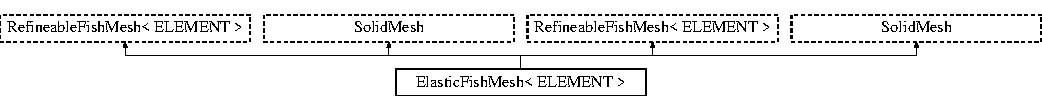
\includegraphics[height=2.000000cm]{classElasticFishMesh}
\end{center}
\end{figure}
\subsection*{Public Member Functions}
\begin{DoxyCompactItemize}
\item 
\hyperlink{classElasticFishMesh_a76c4d63d48b9ee48c3742e55057cfba0}{Elastic\+Fish\+Mesh} (Geom\+Object $\ast$back\+\_\+pt, Geom\+Object $\ast$undeformed\+\_\+back\+\_\+pt, Time\+Stepper $\ast$time\+\_\+stepper\+\_\+pt=\&Mesh\+::\+Default\+\_\+\+Time\+Stepper)
\begin{DoxyCompactList}\small\item\em Constructor\+: Build underlying adaptive fish mesh and then set current Eulerian coordinates to be the Lagrangian ones. Pass pointer to geometric objects that specify the fish\textquotesingle{}s back in the \char`\"{}current\char`\"{} and \char`\"{}undeformed\char`\"{} configurations, and pointer to timestepper (defaults to Static) \end{DoxyCompactList}\item 
virtual \hyperlink{classElasticFishMesh_ab8e084bb7551b9765b95dc38e82ab1be}{$\sim$\+Elastic\+Fish\+Mesh} ()
\begin{DoxyCompactList}\small\item\em Destructor\+: Kill \char`\"{}undeformed\char`\"{} Domain. \end{DoxyCompactList}\end{DoxyCompactItemize}
\subsection*{Private Attributes}
\begin{DoxyCompactItemize}
\item 
Domain $\ast$ \hyperlink{classElasticFishMesh_aef83429a56e87c7218275c1da6c57087}{Undeformed\+\_\+domain\+\_\+pt}
\end{DoxyCompactItemize}


\subsection{Detailed Description}
\subsubsection*{template$<$class E\+L\+E\+M\+E\+NT$>$\newline
class Elastic\+Fish\+Mesh$<$ E\+L\+E\+M\+E\+N\+T $>$}

Refineable fish mesh upgraded to become a solid mesh. 

Definition at line 57 of file static\+\_\+fish.\+cc.



\subsection{Constructor \& Destructor Documentation}
\mbox{\Hypertarget{classElasticFishMesh_a76c4d63d48b9ee48c3742e55057cfba0}\label{classElasticFishMesh_a76c4d63d48b9ee48c3742e55057cfba0}} 
\index{Elastic\+Fish\+Mesh@{Elastic\+Fish\+Mesh}!Elastic\+Fish\+Mesh@{Elastic\+Fish\+Mesh}}
\index{Elastic\+Fish\+Mesh@{Elastic\+Fish\+Mesh}!Elastic\+Fish\+Mesh@{Elastic\+Fish\+Mesh}}
\subsubsection{\texorpdfstring{Elastic\+Fish\+Mesh()}{ElasticFishMesh()}}
{\footnotesize\ttfamily template$<$class E\+L\+E\+M\+E\+NT$>$ \\
\hyperlink{classElasticFishMesh}{Elastic\+Fish\+Mesh}$<$ E\+L\+E\+M\+E\+NT $>$\+::\hyperlink{classElasticFishMesh}{Elastic\+Fish\+Mesh} (\begin{DoxyParamCaption}\item[{Geom\+Object $\ast$}]{back\+\_\+pt,  }\item[{Geom\+Object $\ast$}]{undeformed\+\_\+back\+\_\+pt,  }\item[{Time\+Stepper $\ast$}]{time\+\_\+stepper\+\_\+pt = {\ttfamily \&Mesh\+:\+:Default\+\_\+TimeStepper} }\end{DoxyParamCaption})\hspace{0.3cm}{\ttfamily [inline]}}



Constructor\+: Build underlying adaptive fish mesh and then set current Eulerian coordinates to be the Lagrangian ones. Pass pointer to geometric objects that specify the fish\textquotesingle{}s back in the \char`\"{}current\char`\"{} and \char`\"{}undeformed\char`\"{} configurations, and pointer to timestepper (defaults to Static) 



Definition at line 72 of file static\+\_\+fish.\+cc.

\mbox{\Hypertarget{classElasticFishMesh_ab8e084bb7551b9765b95dc38e82ab1be}\label{classElasticFishMesh_ab8e084bb7551b9765b95dc38e82ab1be}} 
\index{Elastic\+Fish\+Mesh@{Elastic\+Fish\+Mesh}!````~Elastic\+Fish\+Mesh@{$\sim$\+Elastic\+Fish\+Mesh}}
\index{````~Elastic\+Fish\+Mesh@{$\sim$\+Elastic\+Fish\+Mesh}!Elastic\+Fish\+Mesh@{Elastic\+Fish\+Mesh}}
\subsubsection{\texorpdfstring{$\sim$\+Elastic\+Fish\+Mesh()}{~ElasticFishMesh()}}
{\footnotesize\ttfamily template$<$class E\+L\+E\+M\+E\+NT$>$ \\
virtual \hyperlink{classElasticFishMesh}{Elastic\+Fish\+Mesh}$<$ E\+L\+E\+M\+E\+NT $>$\+::$\sim$\hyperlink{classElasticFishMesh}{Elastic\+Fish\+Mesh} (\begin{DoxyParamCaption}{ }\end{DoxyParamCaption})\hspace{0.3cm}{\ttfamily [inline]}, {\ttfamily [virtual]}}



Destructor\+: Kill \char`\"{}undeformed\char`\"{} Domain. 



Definition at line 115 of file static\+\_\+fish.\+cc.



\subsection{Member Data Documentation}
\mbox{\Hypertarget{classElasticFishMesh_aef83429a56e87c7218275c1da6c57087}\label{classElasticFishMesh_aef83429a56e87c7218275c1da6c57087}} 
\index{Elastic\+Fish\+Mesh@{Elastic\+Fish\+Mesh}!Undeformed\+\_\+domain\+\_\+pt@{Undeformed\+\_\+domain\+\_\+pt}}
\index{Undeformed\+\_\+domain\+\_\+pt@{Undeformed\+\_\+domain\+\_\+pt}!Elastic\+Fish\+Mesh@{Elastic\+Fish\+Mesh}}
\subsubsection{\texorpdfstring{Undeformed\+\_\+domain\+\_\+pt}{Undeformed\_domain\_pt}}
{\footnotesize\ttfamily template$<$class E\+L\+E\+M\+E\+NT$>$ \\
Domain$\ast$ \hyperlink{classElasticFishMesh}{Elastic\+Fish\+Mesh}$<$ E\+L\+E\+M\+E\+NT $>$\+::Undeformed\+\_\+domain\+\_\+pt\hspace{0.3cm}{\ttfamily [private]}}

Pointer to \char`\"{}undeformed\char`\"{} Domain -- used to determine the Lagrangian coordinates of any newly created Solid\+Nodes during Mesh refinement 

Definition at line 126 of file static\+\_\+fish.\+cc.



The documentation for this class was generated from the following file\+:\begin{DoxyCompactItemize}
\item 
\hyperlink{static__fish_8cc}{static\+\_\+fish.\+cc}\end{DoxyCompactItemize}

\hypertarget{classFreeBoundaryPoissonProblem}{}\section{Free\+Boundary\+Poisson\+Problem$<$ E\+L\+E\+M\+E\+NT $>$ Class Template Reference}
\label{classFreeBoundaryPoissonProblem}\index{Free\+Boundary\+Poisson\+Problem$<$ E\+L\+E\+M\+E\+N\+T $>$@{Free\+Boundary\+Poisson\+Problem$<$ E\+L\+E\+M\+E\+N\+T $>$}}
Inheritance diagram for Free\+Boundary\+Poisson\+Problem$<$ E\+L\+E\+M\+E\+NT $>$\+:\begin{figure}[H]
\begin{center}
\leavevmode
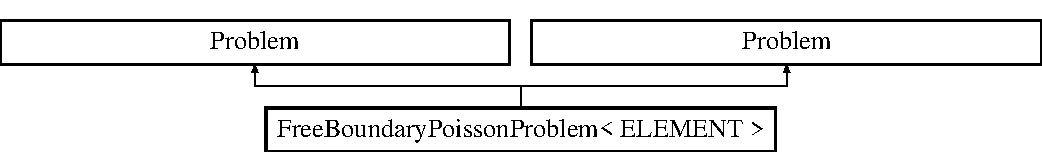
\includegraphics[height=2.000000cm]{classFreeBoundaryPoissonProblem}
\end{center}
\end{figure}
\subsection*{Public Member Functions}
\begin{DoxyCompactItemize}
\item 
\hyperlink{classFreeBoundaryPoissonProblem_a0efe7c342eea790fc0240830bc3c4ebc}{Free\+Boundary\+Poisson\+Problem} ()
\begin{DoxyCompactList}\small\item\em Constructor. \end{DoxyCompactList}\item 
virtual \hyperlink{classFreeBoundaryPoissonProblem_a5b75b8553f3dfed4e9a8996c1b13edf3}{$\sim$\+Free\+Boundary\+Poisson\+Problem} ()
\begin{DoxyCompactList}\small\item\em Destructor (empty) \end{DoxyCompactList}\item 
void \hyperlink{classFreeBoundaryPoissonProblem_aeef57bd5dc79b6aba9eeadcd0c01a2e0}{actions\+\_\+before\+\_\+newton\+\_\+solve} ()
\begin{DoxyCompactList}\small\item\em Update the problem specs before solve (empty) \end{DoxyCompactList}\item 
void \hyperlink{classFreeBoundaryPoissonProblem_aa18df6c9a9287f67ae1bff0f67aaa625}{actions\+\_\+after\+\_\+newton\+\_\+solve} ()
\begin{DoxyCompactList}\small\item\em Update the problem specs after solve (empty) \end{DoxyCompactList}\item 
\hyperlink{classMyMacroElementNodeUpdateRefineableFishMesh}{My\+Macro\+Element\+Node\+Update\+Refineable\+Fish\+Mesh}$<$ E\+L\+E\+M\+E\+NT $>$ $\ast$ \hyperlink{classFreeBoundaryPoissonProblem_adccab51afed9228783120934b6be37c9}{fish\+\_\+mesh\+\_\+pt} ()
\begin{DoxyCompactList}\small\item\em Access function for the fish mesh. \end{DoxyCompactList}\item 
void \hyperlink{classFreeBoundaryPoissonProblem_a2282d8ac1d5753771a9a3cfc0417f6b6}{doc\+\_\+solution} ()
\begin{DoxyCompactList}\small\item\em Doc the solution. \end{DoxyCompactList}\item 
void \hyperlink{classFreeBoundaryPoissonProblem_a885a6e3a4efd1f02314806dced566569}{actions\+\_\+before\+\_\+newton\+\_\+convergence\+\_\+check} ()
\begin{DoxyCompactList}\small\item\em Before checking the new residuals in Newton\textquotesingle{}s method we have to update nodal positions in response to possible changes in the position of the domain boundary. \end{DoxyCompactList}\item 
\hyperlink{classFreeBoundaryPoissonProblem_a0efe7c342eea790fc0240830bc3c4ebc}{Free\+Boundary\+Poisson\+Problem} ()
\begin{DoxyCompactList}\small\item\em Constructor. \end{DoxyCompactList}\item 
virtual \hyperlink{classFreeBoundaryPoissonProblem_a5b75b8553f3dfed4e9a8996c1b13edf3}{$\sim$\+Free\+Boundary\+Poisson\+Problem} ()
\begin{DoxyCompactList}\small\item\em Destructor (empty) \end{DoxyCompactList}\item 
void \hyperlink{classFreeBoundaryPoissonProblem_aeef57bd5dc79b6aba9eeadcd0c01a2e0}{actions\+\_\+before\+\_\+newton\+\_\+solve} ()
\begin{DoxyCompactList}\small\item\em Update the problem specs before solve (empty) \end{DoxyCompactList}\item 
void \hyperlink{classFreeBoundaryPoissonProblem_aa18df6c9a9287f67ae1bff0f67aaa625}{actions\+\_\+after\+\_\+newton\+\_\+solve} ()
\begin{DoxyCompactList}\small\item\em Update the problem specs after solve (empty) \end{DoxyCompactList}\item 
\hyperlink{classMyMacroElementNodeUpdateFishMesh}{My\+Macro\+Element\+Node\+Update\+Fish\+Mesh}$<$ E\+L\+E\+M\+E\+NT $>$ $\ast$ \hyperlink{classFreeBoundaryPoissonProblem_a2e5bc4d52a7d8feefc2aafae0fd29bab}{fish\+\_\+mesh\+\_\+pt} ()
\begin{DoxyCompactList}\small\item\em Access function for the fish mesh. \end{DoxyCompactList}\item 
void \hyperlink{classFreeBoundaryPoissonProblem_a2282d8ac1d5753771a9a3cfc0417f6b6}{doc\+\_\+solution} ()
\begin{DoxyCompactList}\small\item\em Doc the solution. \end{DoxyCompactList}\item 
void \hyperlink{classFreeBoundaryPoissonProblem_a885a6e3a4efd1f02314806dced566569}{actions\+\_\+before\+\_\+newton\+\_\+convergence\+\_\+check} ()
\begin{DoxyCompactList}\small\item\em Before checking the new residuals in Newton\textquotesingle{}s method we have to update nodal positions in response to possible changes in the position of the domain boundary. \end{DoxyCompactList}\end{DoxyCompactItemize}
\subsection*{Private Attributes}
\begin{DoxyCompactItemize}
\item 
\hyperlink{classMyMacroElementNodeUpdateRefineableFishMesh}{My\+Macro\+Element\+Node\+Update\+Refineable\+Fish\+Mesh}$<$ E\+L\+E\+M\+E\+NT $>$ $\ast$ \hyperlink{classFreeBoundaryPoissonProblem_ae81a7e22c2c61854696b80a94053a663}{Fish\+\_\+mesh\+\_\+pt}
\begin{DoxyCompactList}\small\item\em Pointer to fish mesh. \end{DoxyCompactList}\item 
Mesh $\ast$ \hyperlink{classFreeBoundaryPoissonProblem_aaa45902e79f963060b4b6820c5383cfc}{Fish\+\_\+back\+\_\+mesh\+\_\+pt}
\item 
\hyperlink{classMyMacroElementNodeUpdateFishMesh}{My\+Macro\+Element\+Node\+Update\+Fish\+Mesh}$<$ E\+L\+E\+M\+E\+NT $>$ $\ast$ \hyperlink{classFreeBoundaryPoissonProblem_a625f90221f74269b3ebc8ea6d0035feb}{Fish\+\_\+mesh\+\_\+pt}
\begin{DoxyCompactList}\small\item\em Pointer to fish mesh. \end{DoxyCompactList}\end{DoxyCompactItemize}


\subsection{Detailed Description}
\subsubsection*{template$<$class E\+L\+E\+M\+E\+NT$>$\newline
class Free\+Boundary\+Poisson\+Problem$<$ E\+L\+E\+M\+E\+N\+T $>$}

Refineable \char`\"{}free-\/boundary\char`\"{} Poisson problem in deformable fish-\/shaped domain. Template parameter identifies the element.

Non-\/refineable \char`\"{}free-\/boundary\char`\"{} Poisson problem in deformable fish-\/shaped domain. Template parameter identifies the element. 

Definition at line 150 of file macro\+\_\+element\+\_\+free\+\_\+boundary\+\_\+poisson.\+cc.



\subsection{Constructor \& Destructor Documentation}
\mbox{\Hypertarget{classFreeBoundaryPoissonProblem_a0efe7c342eea790fc0240830bc3c4ebc}\label{classFreeBoundaryPoissonProblem_a0efe7c342eea790fc0240830bc3c4ebc}} 
\index{Free\+Boundary\+Poisson\+Problem@{Free\+Boundary\+Poisson\+Problem}!Free\+Boundary\+Poisson\+Problem@{Free\+Boundary\+Poisson\+Problem}}
\index{Free\+Boundary\+Poisson\+Problem@{Free\+Boundary\+Poisson\+Problem}!Free\+Boundary\+Poisson\+Problem@{Free\+Boundary\+Poisson\+Problem}}
\subsubsection{\texorpdfstring{Free\+Boundary\+Poisson\+Problem()}{FreeBoundaryPoissonProblem()}\hspace{0.1cm}{\footnotesize\ttfamily [1/2]}}
{\footnotesize\ttfamily template$<$class E\+L\+E\+M\+E\+NT $>$ \\
\hyperlink{classFreeBoundaryPoissonProblem}{Free\+Boundary\+Poisson\+Problem}$<$ E\+L\+E\+M\+E\+NT $>$\+::\hyperlink{classFreeBoundaryPoissonProblem}{Free\+Boundary\+Poisson\+Problem} (\begin{DoxyParamCaption}{ }\end{DoxyParamCaption})}



Constructor. 

Constructor for adaptive free-\/boundary Poisson problem in deformable fish-\/shaped domain. Loop over elements and set pointers to source function 

Definition at line 203 of file macro\+\_\+element\+\_\+free\+\_\+boundary\+\_\+poisson.\+cc.



References Const\+Source\+For\+Poisson\+::get\+\_\+source().

\mbox{\Hypertarget{classFreeBoundaryPoissonProblem_a5b75b8553f3dfed4e9a8996c1b13edf3}\label{classFreeBoundaryPoissonProblem_a5b75b8553f3dfed4e9a8996c1b13edf3}} 
\index{Free\+Boundary\+Poisson\+Problem@{Free\+Boundary\+Poisson\+Problem}!````~Free\+Boundary\+Poisson\+Problem@{$\sim$\+Free\+Boundary\+Poisson\+Problem}}
\index{````~Free\+Boundary\+Poisson\+Problem@{$\sim$\+Free\+Boundary\+Poisson\+Problem}!Free\+Boundary\+Poisson\+Problem@{Free\+Boundary\+Poisson\+Problem}}
\subsubsection{\texorpdfstring{$\sim$\+Free\+Boundary\+Poisson\+Problem()}{~FreeBoundaryPoissonProblem()}\hspace{0.1cm}{\footnotesize\ttfamily [1/2]}}
{\footnotesize\ttfamily template$<$class E\+L\+E\+M\+E\+NT$>$ \\
virtual \hyperlink{classFreeBoundaryPoissonProblem}{Free\+Boundary\+Poisson\+Problem}$<$ E\+L\+E\+M\+E\+NT $>$\+::$\sim$\hyperlink{classFreeBoundaryPoissonProblem}{Free\+Boundary\+Poisson\+Problem} (\begin{DoxyParamCaption}{ }\end{DoxyParamCaption})\hspace{0.3cm}{\ttfamily [inline]}, {\ttfamily [virtual]}}



Destructor (empty) 



Definition at line 159 of file macro\+\_\+element\+\_\+free\+\_\+boundary\+\_\+poisson.\+cc.

\mbox{\Hypertarget{classFreeBoundaryPoissonProblem_a0efe7c342eea790fc0240830bc3c4ebc}\label{classFreeBoundaryPoissonProblem_a0efe7c342eea790fc0240830bc3c4ebc}} 
\index{Free\+Boundary\+Poisson\+Problem@{Free\+Boundary\+Poisson\+Problem}!Free\+Boundary\+Poisson\+Problem@{Free\+Boundary\+Poisson\+Problem}}
\index{Free\+Boundary\+Poisson\+Problem@{Free\+Boundary\+Poisson\+Problem}!Free\+Boundary\+Poisson\+Problem@{Free\+Boundary\+Poisson\+Problem}}
\subsubsection{\texorpdfstring{Free\+Boundary\+Poisson\+Problem()}{FreeBoundaryPoissonProblem()}\hspace{0.1cm}{\footnotesize\ttfamily [2/2]}}
{\footnotesize\ttfamily template$<$class E\+L\+E\+M\+E\+NT$>$ \\
\hyperlink{classFreeBoundaryPoissonProblem}{Free\+Boundary\+Poisson\+Problem}$<$ E\+L\+E\+M\+E\+NT $>$\+::\hyperlink{classFreeBoundaryPoissonProblem}{Free\+Boundary\+Poisson\+Problem} (\begin{DoxyParamCaption}{ }\end{DoxyParamCaption})}



Constructor. 

\mbox{\Hypertarget{classFreeBoundaryPoissonProblem_a5b75b8553f3dfed4e9a8996c1b13edf3}\label{classFreeBoundaryPoissonProblem_a5b75b8553f3dfed4e9a8996c1b13edf3}} 
\index{Free\+Boundary\+Poisson\+Problem@{Free\+Boundary\+Poisson\+Problem}!````~Free\+Boundary\+Poisson\+Problem@{$\sim$\+Free\+Boundary\+Poisson\+Problem}}
\index{````~Free\+Boundary\+Poisson\+Problem@{$\sim$\+Free\+Boundary\+Poisson\+Problem}!Free\+Boundary\+Poisson\+Problem@{Free\+Boundary\+Poisson\+Problem}}
\subsubsection{\texorpdfstring{$\sim$\+Free\+Boundary\+Poisson\+Problem()}{~FreeBoundaryPoissonProblem()}\hspace{0.1cm}{\footnotesize\ttfamily [2/2]}}
{\footnotesize\ttfamily template$<$class E\+L\+E\+M\+E\+NT$>$ \\
virtual \hyperlink{classFreeBoundaryPoissonProblem}{Free\+Boundary\+Poisson\+Problem}$<$ E\+L\+E\+M\+E\+NT $>$\+::$\sim$\hyperlink{classFreeBoundaryPoissonProblem}{Free\+Boundary\+Poisson\+Problem} (\begin{DoxyParamCaption}{ }\end{DoxyParamCaption})\hspace{0.3cm}{\ttfamily [inline]}, {\ttfamily [virtual]}}



Destructor (empty) 



Definition at line 155 of file macro\+\_\+element\+\_\+free\+\_\+boundary\+\_\+poisson\+\_\+non\+\_\+ref.\+cc.



\subsection{Member Function Documentation}
\mbox{\Hypertarget{classFreeBoundaryPoissonProblem_aa18df6c9a9287f67ae1bff0f67aaa625}\label{classFreeBoundaryPoissonProblem_aa18df6c9a9287f67ae1bff0f67aaa625}} 
\index{Free\+Boundary\+Poisson\+Problem@{Free\+Boundary\+Poisson\+Problem}!actions\+\_\+after\+\_\+newton\+\_\+solve@{actions\+\_\+after\+\_\+newton\+\_\+solve}}
\index{actions\+\_\+after\+\_\+newton\+\_\+solve@{actions\+\_\+after\+\_\+newton\+\_\+solve}!Free\+Boundary\+Poisson\+Problem@{Free\+Boundary\+Poisson\+Problem}}
\subsubsection{\texorpdfstring{actions\+\_\+after\+\_\+newton\+\_\+solve()}{actions\_after\_newton\_solve()}\hspace{0.1cm}{\footnotesize\ttfamily [1/2]}}
{\footnotesize\ttfamily template$<$class E\+L\+E\+M\+E\+NT$>$ \\
void \hyperlink{classFreeBoundaryPoissonProblem}{Free\+Boundary\+Poisson\+Problem}$<$ E\+L\+E\+M\+E\+NT $>$\+::actions\+\_\+after\+\_\+newton\+\_\+solve (\begin{DoxyParamCaption}{ }\end{DoxyParamCaption})\hspace{0.3cm}{\ttfamily [inline]}}



Update the problem specs after solve (empty) 



Definition at line 161 of file macro\+\_\+element\+\_\+free\+\_\+boundary\+\_\+poisson\+\_\+non\+\_\+ref.\+cc.

\mbox{\Hypertarget{classFreeBoundaryPoissonProblem_aa18df6c9a9287f67ae1bff0f67aaa625}\label{classFreeBoundaryPoissonProblem_aa18df6c9a9287f67ae1bff0f67aaa625}} 
\index{Free\+Boundary\+Poisson\+Problem@{Free\+Boundary\+Poisson\+Problem}!actions\+\_\+after\+\_\+newton\+\_\+solve@{actions\+\_\+after\+\_\+newton\+\_\+solve}}
\index{actions\+\_\+after\+\_\+newton\+\_\+solve@{actions\+\_\+after\+\_\+newton\+\_\+solve}!Free\+Boundary\+Poisson\+Problem@{Free\+Boundary\+Poisson\+Problem}}
\subsubsection{\texorpdfstring{actions\+\_\+after\+\_\+newton\+\_\+solve()}{actions\_after\_newton\_solve()}\hspace{0.1cm}{\footnotesize\ttfamily [2/2]}}
{\footnotesize\ttfamily template$<$class E\+L\+E\+M\+E\+NT$>$ \\
void \hyperlink{classFreeBoundaryPoissonProblem}{Free\+Boundary\+Poisson\+Problem}$<$ E\+L\+E\+M\+E\+NT $>$\+::actions\+\_\+after\+\_\+newton\+\_\+solve (\begin{DoxyParamCaption}{ }\end{DoxyParamCaption})\hspace{0.3cm}{\ttfamily [inline]}}



Update the problem specs after solve (empty) 



Definition at line 165 of file macro\+\_\+element\+\_\+free\+\_\+boundary\+\_\+poisson.\+cc.

\mbox{\Hypertarget{classFreeBoundaryPoissonProblem_a885a6e3a4efd1f02314806dced566569}\label{classFreeBoundaryPoissonProblem_a885a6e3a4efd1f02314806dced566569}} 
\index{Free\+Boundary\+Poisson\+Problem@{Free\+Boundary\+Poisson\+Problem}!actions\+\_\+before\+\_\+newton\+\_\+convergence\+\_\+check@{actions\+\_\+before\+\_\+newton\+\_\+convergence\+\_\+check}}
\index{actions\+\_\+before\+\_\+newton\+\_\+convergence\+\_\+check@{actions\+\_\+before\+\_\+newton\+\_\+convergence\+\_\+check}!Free\+Boundary\+Poisson\+Problem@{Free\+Boundary\+Poisson\+Problem}}
\subsubsection{\texorpdfstring{actions\+\_\+before\+\_\+newton\+\_\+convergence\+\_\+check()}{actions\_before\_newton\_convergence\_check()}\hspace{0.1cm}{\footnotesize\ttfamily [1/2]}}
{\footnotesize\ttfamily template$<$class E\+L\+E\+M\+E\+NT$>$ \\
void \hyperlink{classFreeBoundaryPoissonProblem}{Free\+Boundary\+Poisson\+Problem}$<$ E\+L\+E\+M\+E\+NT $>$\+::actions\+\_\+before\+\_\+newton\+\_\+convergence\+\_\+check (\begin{DoxyParamCaption}{ }\end{DoxyParamCaption})\hspace{0.3cm}{\ttfamily [inline]}}



Before checking the new residuals in Newton\textquotesingle{}s method we have to update nodal positions in response to possible changes in the position of the domain boundary. 



Definition at line 175 of file macro\+\_\+element\+\_\+free\+\_\+boundary\+\_\+poisson\+\_\+non\+\_\+ref.\+cc.

\mbox{\Hypertarget{classFreeBoundaryPoissonProblem_a885a6e3a4efd1f02314806dced566569}\label{classFreeBoundaryPoissonProblem_a885a6e3a4efd1f02314806dced566569}} 
\index{Free\+Boundary\+Poisson\+Problem@{Free\+Boundary\+Poisson\+Problem}!actions\+\_\+before\+\_\+newton\+\_\+convergence\+\_\+check@{actions\+\_\+before\+\_\+newton\+\_\+convergence\+\_\+check}}
\index{actions\+\_\+before\+\_\+newton\+\_\+convergence\+\_\+check@{actions\+\_\+before\+\_\+newton\+\_\+convergence\+\_\+check}!Free\+Boundary\+Poisson\+Problem@{Free\+Boundary\+Poisson\+Problem}}
\subsubsection{\texorpdfstring{actions\+\_\+before\+\_\+newton\+\_\+convergence\+\_\+check()}{actions\_before\_newton\_convergence\_check()}\hspace{0.1cm}{\footnotesize\ttfamily [2/2]}}
{\footnotesize\ttfamily template$<$class E\+L\+E\+M\+E\+NT$>$ \\
void \hyperlink{classFreeBoundaryPoissonProblem}{Free\+Boundary\+Poisson\+Problem}$<$ E\+L\+E\+M\+E\+NT $>$\+::actions\+\_\+before\+\_\+newton\+\_\+convergence\+\_\+check (\begin{DoxyParamCaption}{ }\end{DoxyParamCaption})\hspace{0.3cm}{\ttfamily [inline]}}



Before checking the new residuals in Newton\textquotesingle{}s method we have to update nodal positions in response to possible changes in the position of the domain boundary. 



Definition at line 179 of file macro\+\_\+element\+\_\+free\+\_\+boundary\+\_\+poisson.\+cc.

\mbox{\Hypertarget{classFreeBoundaryPoissonProblem_aeef57bd5dc79b6aba9eeadcd0c01a2e0}\label{classFreeBoundaryPoissonProblem_aeef57bd5dc79b6aba9eeadcd0c01a2e0}} 
\index{Free\+Boundary\+Poisson\+Problem@{Free\+Boundary\+Poisson\+Problem}!actions\+\_\+before\+\_\+newton\+\_\+solve@{actions\+\_\+before\+\_\+newton\+\_\+solve}}
\index{actions\+\_\+before\+\_\+newton\+\_\+solve@{actions\+\_\+before\+\_\+newton\+\_\+solve}!Free\+Boundary\+Poisson\+Problem@{Free\+Boundary\+Poisson\+Problem}}
\subsubsection{\texorpdfstring{actions\+\_\+before\+\_\+newton\+\_\+solve()}{actions\_before\_newton\_solve()}\hspace{0.1cm}{\footnotesize\ttfamily [1/2]}}
{\footnotesize\ttfamily template$<$class E\+L\+E\+M\+E\+NT$>$ \\
void \hyperlink{classFreeBoundaryPoissonProblem}{Free\+Boundary\+Poisson\+Problem}$<$ E\+L\+E\+M\+E\+NT $>$\+::actions\+\_\+before\+\_\+newton\+\_\+solve (\begin{DoxyParamCaption}{ }\end{DoxyParamCaption})\hspace{0.3cm}{\ttfamily [inline]}}



Update the problem specs before solve (empty) 



Definition at line 158 of file macro\+\_\+element\+\_\+free\+\_\+boundary\+\_\+poisson\+\_\+non\+\_\+ref.\+cc.

\mbox{\Hypertarget{classFreeBoundaryPoissonProblem_aeef57bd5dc79b6aba9eeadcd0c01a2e0}\label{classFreeBoundaryPoissonProblem_aeef57bd5dc79b6aba9eeadcd0c01a2e0}} 
\index{Free\+Boundary\+Poisson\+Problem@{Free\+Boundary\+Poisson\+Problem}!actions\+\_\+before\+\_\+newton\+\_\+solve@{actions\+\_\+before\+\_\+newton\+\_\+solve}}
\index{actions\+\_\+before\+\_\+newton\+\_\+solve@{actions\+\_\+before\+\_\+newton\+\_\+solve}!Free\+Boundary\+Poisson\+Problem@{Free\+Boundary\+Poisson\+Problem}}
\subsubsection{\texorpdfstring{actions\+\_\+before\+\_\+newton\+\_\+solve()}{actions\_before\_newton\_solve()}\hspace{0.1cm}{\footnotesize\ttfamily [2/2]}}
{\footnotesize\ttfamily template$<$class E\+L\+E\+M\+E\+NT$>$ \\
void \hyperlink{classFreeBoundaryPoissonProblem}{Free\+Boundary\+Poisson\+Problem}$<$ E\+L\+E\+M\+E\+NT $>$\+::actions\+\_\+before\+\_\+newton\+\_\+solve (\begin{DoxyParamCaption}{ }\end{DoxyParamCaption})\hspace{0.3cm}{\ttfamily [inline]}}



Update the problem specs before solve (empty) 



Definition at line 162 of file macro\+\_\+element\+\_\+free\+\_\+boundary\+\_\+poisson.\+cc.

\mbox{\Hypertarget{classFreeBoundaryPoissonProblem_a2282d8ac1d5753771a9a3cfc0417f6b6}\label{classFreeBoundaryPoissonProblem_a2282d8ac1d5753771a9a3cfc0417f6b6}} 
\index{Free\+Boundary\+Poisson\+Problem@{Free\+Boundary\+Poisson\+Problem}!doc\+\_\+solution@{doc\+\_\+solution}}
\index{doc\+\_\+solution@{doc\+\_\+solution}!Free\+Boundary\+Poisson\+Problem@{Free\+Boundary\+Poisson\+Problem}}
\subsubsection{\texorpdfstring{doc\+\_\+solution()}{doc\_solution()}\hspace{0.1cm}{\footnotesize\ttfamily [1/2]}}
{\footnotesize\ttfamily template$<$class E\+L\+E\+M\+E\+NT$>$ \\
void \hyperlink{classFreeBoundaryPoissonProblem}{Free\+Boundary\+Poisson\+Problem}$<$ E\+L\+E\+M\+E\+NT $>$\+::doc\+\_\+solution (\begin{DoxyParamCaption}{ }\end{DoxyParamCaption})}



Doc the solution. 

\mbox{\Hypertarget{classFreeBoundaryPoissonProblem_a2282d8ac1d5753771a9a3cfc0417f6b6}\label{classFreeBoundaryPoissonProblem_a2282d8ac1d5753771a9a3cfc0417f6b6}} 
\index{Free\+Boundary\+Poisson\+Problem@{Free\+Boundary\+Poisson\+Problem}!doc\+\_\+solution@{doc\+\_\+solution}}
\index{doc\+\_\+solution@{doc\+\_\+solution}!Free\+Boundary\+Poisson\+Problem@{Free\+Boundary\+Poisson\+Problem}}
\subsubsection{\texorpdfstring{doc\+\_\+solution()}{doc\_solution()}\hspace{0.1cm}{\footnotesize\ttfamily [2/2]}}
{\footnotesize\ttfamily template$<$class E\+L\+E\+M\+E\+NT $>$ \\
void \hyperlink{classFreeBoundaryPoissonProblem}{Free\+Boundary\+Poisson\+Problem}$<$ E\+L\+E\+M\+E\+NT $>$\+::doc\+\_\+solution (\begin{DoxyParamCaption}{ }\end{DoxyParamCaption})}



Doc the solution. 

Doc the solution in tecplot format. 

Definition at line 292 of file macro\+\_\+element\+\_\+free\+\_\+boundary\+\_\+poisson.\+cc.



Referenced by main().

\mbox{\Hypertarget{classFreeBoundaryPoissonProblem_a2e5bc4d52a7d8feefc2aafae0fd29bab}\label{classFreeBoundaryPoissonProblem_a2e5bc4d52a7d8feefc2aafae0fd29bab}} 
\index{Free\+Boundary\+Poisson\+Problem@{Free\+Boundary\+Poisson\+Problem}!fish\+\_\+mesh\+\_\+pt@{fish\+\_\+mesh\+\_\+pt}}
\index{fish\+\_\+mesh\+\_\+pt@{fish\+\_\+mesh\+\_\+pt}!Free\+Boundary\+Poisson\+Problem@{Free\+Boundary\+Poisson\+Problem}}
\subsubsection{\texorpdfstring{fish\+\_\+mesh\+\_\+pt()}{fish\_mesh\_pt()}\hspace{0.1cm}{\footnotesize\ttfamily [1/2]}}
{\footnotesize\ttfamily template$<$class E\+L\+E\+M\+E\+NT$>$ \\
\hyperlink{classMyMacroElementNodeUpdateFishMesh}{My\+Macro\+Element\+Node\+Update\+Fish\+Mesh}$<$E\+L\+E\+M\+E\+NT$>$$\ast$ \hyperlink{classFreeBoundaryPoissonProblem}{Free\+Boundary\+Poisson\+Problem}$<$ E\+L\+E\+M\+E\+NT $>$\+::fish\+\_\+mesh\+\_\+pt (\begin{DoxyParamCaption}{ }\end{DoxyParamCaption})\hspace{0.3cm}{\ttfamily [inline]}}



Access function for the fish mesh. 



Definition at line 164 of file macro\+\_\+element\+\_\+free\+\_\+boundary\+\_\+poisson\+\_\+non\+\_\+ref.\+cc.

\mbox{\Hypertarget{classFreeBoundaryPoissonProblem_adccab51afed9228783120934b6be37c9}\label{classFreeBoundaryPoissonProblem_adccab51afed9228783120934b6be37c9}} 
\index{Free\+Boundary\+Poisson\+Problem@{Free\+Boundary\+Poisson\+Problem}!fish\+\_\+mesh\+\_\+pt@{fish\+\_\+mesh\+\_\+pt}}
\index{fish\+\_\+mesh\+\_\+pt@{fish\+\_\+mesh\+\_\+pt}!Free\+Boundary\+Poisson\+Problem@{Free\+Boundary\+Poisson\+Problem}}
\subsubsection{\texorpdfstring{fish\+\_\+mesh\+\_\+pt()}{fish\_mesh\_pt()}\hspace{0.1cm}{\footnotesize\ttfamily [2/2]}}
{\footnotesize\ttfamily template$<$class E\+L\+E\+M\+E\+NT$>$ \\
\hyperlink{classMyMacroElementNodeUpdateRefineableFishMesh}{My\+Macro\+Element\+Node\+Update\+Refineable\+Fish\+Mesh}$<$E\+L\+E\+M\+E\+NT$>$$\ast$ \hyperlink{classFreeBoundaryPoissonProblem}{Free\+Boundary\+Poisson\+Problem}$<$ E\+L\+E\+M\+E\+NT $>$\+::fish\+\_\+mesh\+\_\+pt (\begin{DoxyParamCaption}{ }\end{DoxyParamCaption})\hspace{0.3cm}{\ttfamily [inline]}}



Access function for the fish mesh. 



Definition at line 168 of file macro\+\_\+element\+\_\+free\+\_\+boundary\+\_\+poisson.\+cc.



\subsection{Member Data Documentation}
\mbox{\Hypertarget{classFreeBoundaryPoissonProblem_aaa45902e79f963060b4b6820c5383cfc}\label{classFreeBoundaryPoissonProblem_aaa45902e79f963060b4b6820c5383cfc}} 
\index{Free\+Boundary\+Poisson\+Problem@{Free\+Boundary\+Poisson\+Problem}!Fish\+\_\+back\+\_\+mesh\+\_\+pt@{Fish\+\_\+back\+\_\+mesh\+\_\+pt}}
\index{Fish\+\_\+back\+\_\+mesh\+\_\+pt@{Fish\+\_\+back\+\_\+mesh\+\_\+pt}!Free\+Boundary\+Poisson\+Problem@{Free\+Boundary\+Poisson\+Problem}}
\subsubsection{\texorpdfstring{Fish\+\_\+back\+\_\+mesh\+\_\+pt}{Fish\_back\_mesh\_pt}}
{\footnotesize\ttfamily template$<$class E\+L\+E\+M\+E\+NT$>$ \\
Mesh $\ast$ \hyperlink{classFreeBoundaryPoissonProblem}{Free\+Boundary\+Poisson\+Problem}$<$ E\+L\+E\+M\+E\+NT $>$\+::Fish\+\_\+back\+\_\+mesh\+\_\+pt\hspace{0.3cm}{\ttfamily [private]}}

Pointer to single-\/element mesh that stores the Generalised\+Element that represents the fish\textquotesingle{}s back 

Definition at line 191 of file macro\+\_\+element\+\_\+free\+\_\+boundary\+\_\+poisson.\+cc.

\mbox{\Hypertarget{classFreeBoundaryPoissonProblem_a625f90221f74269b3ebc8ea6d0035feb}\label{classFreeBoundaryPoissonProblem_a625f90221f74269b3ebc8ea6d0035feb}} 
\index{Free\+Boundary\+Poisson\+Problem@{Free\+Boundary\+Poisson\+Problem}!Fish\+\_\+mesh\+\_\+pt@{Fish\+\_\+mesh\+\_\+pt}}
\index{Fish\+\_\+mesh\+\_\+pt@{Fish\+\_\+mesh\+\_\+pt}!Free\+Boundary\+Poisson\+Problem@{Free\+Boundary\+Poisson\+Problem}}
\subsubsection{\texorpdfstring{Fish\+\_\+mesh\+\_\+pt}{Fish\_mesh\_pt}\hspace{0.1cm}{\footnotesize\ttfamily [1/2]}}
{\footnotesize\ttfamily template$<$class E\+L\+E\+M\+E\+NT$>$ \\
\hyperlink{classMyMacroElementNodeUpdateFishMesh}{My\+Macro\+Element\+Node\+Update\+Fish\+Mesh}$<$E\+L\+E\+M\+E\+NT$>$$\ast$ \hyperlink{classFreeBoundaryPoissonProblem}{Free\+Boundary\+Poisson\+Problem}$<$ E\+L\+E\+M\+E\+NT $>$\+::Fish\+\_\+mesh\+\_\+pt\hspace{0.3cm}{\ttfamily [private]}}



Pointer to fish mesh. 



Definition at line 183 of file macro\+\_\+element\+\_\+free\+\_\+boundary\+\_\+poisson\+\_\+non\+\_\+ref.\+cc.

\mbox{\Hypertarget{classFreeBoundaryPoissonProblem_ae81a7e22c2c61854696b80a94053a663}\label{classFreeBoundaryPoissonProblem_ae81a7e22c2c61854696b80a94053a663}} 
\index{Free\+Boundary\+Poisson\+Problem@{Free\+Boundary\+Poisson\+Problem}!Fish\+\_\+mesh\+\_\+pt@{Fish\+\_\+mesh\+\_\+pt}}
\index{Fish\+\_\+mesh\+\_\+pt@{Fish\+\_\+mesh\+\_\+pt}!Free\+Boundary\+Poisson\+Problem@{Free\+Boundary\+Poisson\+Problem}}
\subsubsection{\texorpdfstring{Fish\+\_\+mesh\+\_\+pt}{Fish\_mesh\_pt}\hspace{0.1cm}{\footnotesize\ttfamily [2/2]}}
{\footnotesize\ttfamily template$<$class E\+L\+E\+M\+E\+NT$>$ \\
\hyperlink{classMyMacroElementNodeUpdateRefineableFishMesh}{My\+Macro\+Element\+Node\+Update\+Refineable\+Fish\+Mesh}$<$E\+L\+E\+M\+E\+NT$>$$\ast$ \hyperlink{classFreeBoundaryPoissonProblem}{Free\+Boundary\+Poisson\+Problem}$<$ E\+L\+E\+M\+E\+NT $>$\+::Fish\+\_\+mesh\+\_\+pt\hspace{0.3cm}{\ttfamily [private]}}



Pointer to fish mesh. 



Definition at line 187 of file macro\+\_\+element\+\_\+free\+\_\+boundary\+\_\+poisson.\+cc.



The documentation for this class was generated from the following files\+:\begin{DoxyCompactItemize}
\item 
\hyperlink{macro__element__free__boundary__poisson_8cc}{macro\+\_\+element\+\_\+free\+\_\+boundary\+\_\+poisson.\+cc}\item 
\hyperlink{macro__element__free__boundary__poisson__non__ref_8cc}{macro\+\_\+element\+\_\+free\+\_\+boundary\+\_\+poisson\+\_\+non\+\_\+ref.\+cc}\end{DoxyCompactItemize}

\hypertarget{classoomph_1_1GeneralCircle}{}\section{oomph\+:\+:General\+Circle Class Reference}
\label{classoomph_1_1GeneralCircle}\index{oomph\+::\+General\+Circle@{oomph\+::\+General\+Circle}}


\hyperlink{classoomph_1_1GeneralCircle}{General\+Circle} in 2D space. \[ x = X_c + R \cos(\zeta) \] \[ y = Y_c + R \sin(\zeta) \] The three parameters $ X_c, Y_c $ and $ R $ are represented by Data and can therefore be unknowns in the problem.  




{\ttfamily \#include $<$circle.\+h$>$}

Inheritance diagram for oomph\+:\+:General\+Circle\+:\begin{figure}[H]
\begin{center}
\leavevmode
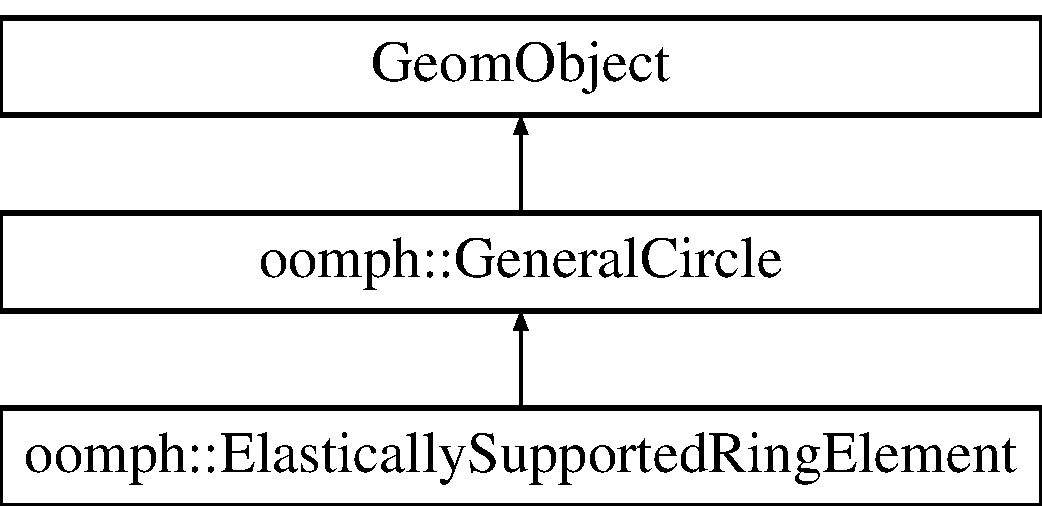
\includegraphics[height=3.000000cm]{classoomph_1_1GeneralCircle}
\end{center}
\end{figure}
\subsection*{Public Member Functions}
\begin{DoxyCompactItemize}
\item 
\hyperlink{classoomph_1_1GeneralCircle_aa4847492eeebdc2033c82734d7bcf2f2}{General\+Circle} (const double \&\hyperlink{classoomph_1_1GeneralCircle_a9c84564d8239bd8b4a2b28649638dd4a}{x\+\_\+c}, const double \&\hyperlink{classoomph_1_1GeneralCircle_afa91b6356920d73e05f81d6e7aaf0bf7}{y\+\_\+c}, const double \&r)
\begin{DoxyCompactList}\small\item\em Constructor\+: Pass x and y-\/coords of centre and radius (all pinned) \end{DoxyCompactList}\item 
\hyperlink{classoomph_1_1GeneralCircle_afdcca2cddb52a51abc693c7d7ba6b173}{General\+Circle} (Data $\ast$\hyperlink{classoomph_1_1GeneralCircle_ad5c33bb9a727a8fe28be0087f5baa9f5}{geom\+\_\+data\+\_\+pt})
\begin{DoxyCompactList}\small\item\em Alternative constructor\+: Pass x and y-\/coords of centre and radius (all as part of Data) \end{DoxyCompactList}\item 
virtual \hyperlink{classoomph_1_1GeneralCircle_a4ba230f7d22d7b116603115952ca50b0}{$\sim$\+General\+Circle} ()
\begin{DoxyCompactList}\small\item\em Destructor\+: Clean up if necessary. \end{DoxyCompactList}\item 
void \hyperlink{classoomph_1_1GeneralCircle_acc120835b4f0c69e7dce7e839db63d1d}{position} (const Vector$<$ double $>$ \&zeta, Vector$<$ double $>$ \&r) const
\begin{DoxyCompactList}\small\item\em Position Vector at Lagrangian coordinate zeta. \end{DoxyCompactList}\item 
void \hyperlink{classoomph_1_1GeneralCircle_a94f7f58a7131f80a245007ff0da73f74}{position} (const unsigned \&t, const Vector$<$ double $>$ \&zeta, Vector$<$ double $>$ \&r) const
\begin{DoxyCompactList}\small\item\em Position Vector at Lagrangian coordinate zeta at time level t (t=0\+: present; t$>$0\+: previous level). Steady object, so we simply forward the call to the steady version. \end{DoxyCompactList}\item 
double \& \hyperlink{classoomph_1_1GeneralCircle_a9c84564d8239bd8b4a2b28649638dd4a}{x\+\_\+c} ()
\begin{DoxyCompactList}\small\item\em Access function to x-\/coordinate of centre of circle. \end{DoxyCompactList}\item 
double \& \hyperlink{classoomph_1_1GeneralCircle_afa91b6356920d73e05f81d6e7aaf0bf7}{y\+\_\+c} ()
\begin{DoxyCompactList}\small\item\em Access function to y-\/coordinate of centre of circle. \end{DoxyCompactList}\item 
double \& \hyperlink{classoomph_1_1GeneralCircle_adc9df8b14326bddb144231b0be5d06c0}{R} ()
\begin{DoxyCompactList}\small\item\em Access function to radius of circle. \end{DoxyCompactList}\item 
unsigned \hyperlink{classoomph_1_1GeneralCircle_a7cd69f069bb8042ba972b89940ec1808}{ngeom\+\_\+data} () const
\begin{DoxyCompactList}\small\item\em How many items of Data does the shape of the object depend on? \end{DoxyCompactList}\item 
Data $\ast$ \hyperlink{classoomph_1_1GeneralCircle_ad5c33bb9a727a8fe28be0087f5baa9f5}{geom\+\_\+data\+\_\+pt} (const unsigned \&j)
\begin{DoxyCompactList}\small\item\em Return pointer to the j-\/th Data item that the object\textquotesingle{}s shape depends on. \end{DoxyCompactList}\end{DoxyCompactItemize}
\subsection*{Protected Attributes}
\begin{DoxyCompactItemize}
\item 
Vector$<$ Data $\ast$ $>$ \hyperlink{classoomph_1_1GeneralCircle_a4a707f37b32d447dbe965177e442aa76}{Geom\+\_\+data\+\_\+pt}
\begin{DoxyCompactList}\small\item\em Vector of pointers to Data items that affects the object\textquotesingle{}s shape. \end{DoxyCompactList}\item 
bool \hyperlink{classoomph_1_1GeneralCircle_a6772cb425079b3afd2479663ddb0cb81}{Must\+\_\+clean\+\_\+up}
\begin{DoxyCompactList}\small\item\em Do I need to clean up? \end{DoxyCompactList}\end{DoxyCompactItemize}


\subsection{Detailed Description}
\hyperlink{classoomph_1_1GeneralCircle}{General\+Circle} in 2D space. \[ x = X_c + R \cos(\zeta) \] \[ y = Y_c + R \sin(\zeta) \] The three parameters $ X_c, Y_c $ and $ R $ are represented by Data and can therefore be unknowns in the problem. 

Definition at line 99 of file circle.\+h.



\subsection{Constructor \& Destructor Documentation}
\mbox{\Hypertarget{classoomph_1_1GeneralCircle_aa4847492eeebdc2033c82734d7bcf2f2}\label{classoomph_1_1GeneralCircle_aa4847492eeebdc2033c82734d7bcf2f2}} 
\index{oomph\+::\+General\+Circle@{oomph\+::\+General\+Circle}!General\+Circle@{General\+Circle}}
\index{General\+Circle@{General\+Circle}!oomph\+::\+General\+Circle@{oomph\+::\+General\+Circle}}
\subsubsection{\texorpdfstring{General\+Circle()}{GeneralCircle()}\hspace{0.1cm}{\footnotesize\ttfamily [1/2]}}
{\footnotesize\ttfamily oomph\+::\+General\+Circle\+::\+General\+Circle (\begin{DoxyParamCaption}\item[{const double \&}]{x\+\_\+c,  }\item[{const double \&}]{y\+\_\+c,  }\item[{const double \&}]{r }\end{DoxyParamCaption})\hspace{0.3cm}{\ttfamily [inline]}}



Constructor\+: Pass x and y-\/coords of centre and radius (all pinned) 



Definition at line 105 of file circle.\+h.

\mbox{\Hypertarget{classoomph_1_1GeneralCircle_afdcca2cddb52a51abc693c7d7ba6b173}\label{classoomph_1_1GeneralCircle_afdcca2cddb52a51abc693c7d7ba6b173}} 
\index{oomph\+::\+General\+Circle@{oomph\+::\+General\+Circle}!General\+Circle@{General\+Circle}}
\index{General\+Circle@{General\+Circle}!oomph\+::\+General\+Circle@{oomph\+::\+General\+Circle}}
\subsubsection{\texorpdfstring{General\+Circle()}{GeneralCircle()}\hspace{0.1cm}{\footnotesize\ttfamily [2/2]}}
{\footnotesize\ttfamily oomph\+::\+General\+Circle\+::\+General\+Circle (\begin{DoxyParamCaption}\item[{Data $\ast$}]{geom\+\_\+data\+\_\+pt }\end{DoxyParamCaption})\hspace{0.3cm}{\ttfamily [inline]}}



Alternative constructor\+: Pass x and y-\/coords of centre and radius (all as part of Data) 


\begin{DoxyCode}
\hyperlink{classoomph_1_1GeneralCircle_a4a707f37b32d447dbe965177e442aa76}{Geom\_data\_pt}[0]->value(0) = X\_c;
\hyperlink{classoomph_1_1GeneralCircle_a4a707f37b32d447dbe965177e442aa76}{Geom\_data\_pt}[0]->value(1) = Y\_c;
\hyperlink{classoomph_1_1GeneralCircle_a4a707f37b32d447dbe965177e442aa76}{Geom\_data\_pt}[0]->value(2) = \hyperlink{classoomph_1_1GeneralCircle_adc9df8b14326bddb144231b0be5d06c0}{R};
\end{DoxyCode}
 

Definition at line 147 of file circle.\+h.

\mbox{\Hypertarget{classoomph_1_1GeneralCircle_a4ba230f7d22d7b116603115952ca50b0}\label{classoomph_1_1GeneralCircle_a4ba230f7d22d7b116603115952ca50b0}} 
\index{oomph\+::\+General\+Circle@{oomph\+::\+General\+Circle}!````~General\+Circle@{$\sim$\+General\+Circle}}
\index{````~General\+Circle@{$\sim$\+General\+Circle}!oomph\+::\+General\+Circle@{oomph\+::\+General\+Circle}}
\subsubsection{\texorpdfstring{$\sim$\+General\+Circle()}{~GeneralCircle()}}
{\footnotesize\ttfamily virtual oomph\+::\+General\+Circle\+::$\sim$\+General\+Circle (\begin{DoxyParamCaption}{ }\end{DoxyParamCaption})\hspace{0.3cm}{\ttfamily [inline]}, {\ttfamily [virtual]}}



Destructor\+: Clean up if necessary. 



Definition at line 171 of file circle.\+h.



\subsection{Member Function Documentation}
\mbox{\Hypertarget{classoomph_1_1GeneralCircle_ad5c33bb9a727a8fe28be0087f5baa9f5}\label{classoomph_1_1GeneralCircle_ad5c33bb9a727a8fe28be0087f5baa9f5}} 
\index{oomph\+::\+General\+Circle@{oomph\+::\+General\+Circle}!geom\+\_\+data\+\_\+pt@{geom\+\_\+data\+\_\+pt}}
\index{geom\+\_\+data\+\_\+pt@{geom\+\_\+data\+\_\+pt}!oomph\+::\+General\+Circle@{oomph\+::\+General\+Circle}}
\subsubsection{\texorpdfstring{geom\+\_\+data\+\_\+pt()}{geom\_data\_pt()}}
{\footnotesize\ttfamily Data$\ast$ oomph\+::\+General\+Circle\+::geom\+\_\+data\+\_\+pt (\begin{DoxyParamCaption}\item[{const unsigned \&}]{j }\end{DoxyParamCaption})\hspace{0.3cm}{\ttfamily [inline]}}



Return pointer to the j-\/th Data item that the object\textquotesingle{}s shape depends on. 



Definition at line 222 of file circle.\+h.

\mbox{\Hypertarget{classoomph_1_1GeneralCircle_a7cd69f069bb8042ba972b89940ec1808}\label{classoomph_1_1GeneralCircle_a7cd69f069bb8042ba972b89940ec1808}} 
\index{oomph\+::\+General\+Circle@{oomph\+::\+General\+Circle}!ngeom\+\_\+data@{ngeom\+\_\+data}}
\index{ngeom\+\_\+data@{ngeom\+\_\+data}!oomph\+::\+General\+Circle@{oomph\+::\+General\+Circle}}
\subsubsection{\texorpdfstring{ngeom\+\_\+data()}{ngeom\_data()}}
{\footnotesize\ttfamily unsigned oomph\+::\+General\+Circle\+::ngeom\+\_\+data (\begin{DoxyParamCaption}{ }\end{DoxyParamCaption}) const\hspace{0.3cm}{\ttfamily [inline]}}



How many items of Data does the shape of the object depend on? 



Definition at line 218 of file circle.\+h.

\mbox{\Hypertarget{classoomph_1_1GeneralCircle_acc120835b4f0c69e7dce7e839db63d1d}\label{classoomph_1_1GeneralCircle_acc120835b4f0c69e7dce7e839db63d1d}} 
\index{oomph\+::\+General\+Circle@{oomph\+::\+General\+Circle}!position@{position}}
\index{position@{position}!oomph\+::\+General\+Circle@{oomph\+::\+General\+Circle}}
\subsubsection{\texorpdfstring{position()}{position()}\hspace{0.1cm}{\footnotesize\ttfamily [1/2]}}
{\footnotesize\ttfamily void oomph\+::\+General\+Circle\+::position (\begin{DoxyParamCaption}\item[{const Vector$<$ double $>$ \&}]{zeta,  }\item[{Vector$<$ double $>$ \&}]{r }\end{DoxyParamCaption}) const\hspace{0.3cm}{\ttfamily [inline]}}



Position Vector at Lagrangian coordinate zeta. 



Definition at line 187 of file circle.\+h.



References oomph\+::\+Simple\+Circle\+::R, oomph\+::\+Simple\+Circle\+::\+X\+\_\+c, and oomph\+::\+Simple\+Circle\+::\+Y\+\_\+c.



Referenced by main().

\mbox{\Hypertarget{classoomph_1_1GeneralCircle_a94f7f58a7131f80a245007ff0da73f74}\label{classoomph_1_1GeneralCircle_a94f7f58a7131f80a245007ff0da73f74}} 
\index{oomph\+::\+General\+Circle@{oomph\+::\+General\+Circle}!position@{position}}
\index{position@{position}!oomph\+::\+General\+Circle@{oomph\+::\+General\+Circle}}
\subsubsection{\texorpdfstring{position()}{position()}\hspace{0.1cm}{\footnotesize\ttfamily [2/2]}}
{\footnotesize\ttfamily void oomph\+::\+General\+Circle\+::position (\begin{DoxyParamCaption}\item[{const unsigned \&}]{t,  }\item[{const Vector$<$ double $>$ \&}]{zeta,  }\item[{Vector$<$ double $>$ \&}]{r }\end{DoxyParamCaption}) const\hspace{0.3cm}{\ttfamily [inline]}}



Position Vector at Lagrangian coordinate zeta at time level t (t=0\+: present; t$>$0\+: previous level). Steady object, so we simply forward the call to the steady version. 



Definition at line 204 of file circle.\+h.



References oomph\+::\+Simple\+Circle\+::position().

\mbox{\Hypertarget{classoomph_1_1GeneralCircle_adc9df8b14326bddb144231b0be5d06c0}\label{classoomph_1_1GeneralCircle_adc9df8b14326bddb144231b0be5d06c0}} 
\index{oomph\+::\+General\+Circle@{oomph\+::\+General\+Circle}!R@{R}}
\index{R@{R}!oomph\+::\+General\+Circle@{oomph\+::\+General\+Circle}}
\subsubsection{\texorpdfstring{R()}{R()}}
{\footnotesize\ttfamily double\& oomph\+::\+General\+Circle\+::R (\begin{DoxyParamCaption}{ }\end{DoxyParamCaption})\hspace{0.3cm}{\ttfamily [inline]}}



Access function to radius of circle. 



Definition at line 215 of file circle.\+h.

\mbox{\Hypertarget{classoomph_1_1GeneralCircle_a9c84564d8239bd8b4a2b28649638dd4a}\label{classoomph_1_1GeneralCircle_a9c84564d8239bd8b4a2b28649638dd4a}} 
\index{oomph\+::\+General\+Circle@{oomph\+::\+General\+Circle}!x\+\_\+c@{x\+\_\+c}}
\index{x\+\_\+c@{x\+\_\+c}!oomph\+::\+General\+Circle@{oomph\+::\+General\+Circle}}
\subsubsection{\texorpdfstring{x\+\_\+c()}{x\_c()}}
{\footnotesize\ttfamily double\& oomph\+::\+General\+Circle\+::x\+\_\+c (\begin{DoxyParamCaption}{ }\end{DoxyParamCaption})\hspace{0.3cm}{\ttfamily [inline]}}



Access function to x-\/coordinate of centre of circle. 



Definition at line 209 of file circle.\+h.

\mbox{\Hypertarget{classoomph_1_1GeneralCircle_afa91b6356920d73e05f81d6e7aaf0bf7}\label{classoomph_1_1GeneralCircle_afa91b6356920d73e05f81d6e7aaf0bf7}} 
\index{oomph\+::\+General\+Circle@{oomph\+::\+General\+Circle}!y\+\_\+c@{y\+\_\+c}}
\index{y\+\_\+c@{y\+\_\+c}!oomph\+::\+General\+Circle@{oomph\+::\+General\+Circle}}
\subsubsection{\texorpdfstring{y\+\_\+c()}{y\_c()}}
{\footnotesize\ttfamily double\& oomph\+::\+General\+Circle\+::y\+\_\+c (\begin{DoxyParamCaption}{ }\end{DoxyParamCaption})\hspace{0.3cm}{\ttfamily [inline]}}



Access function to y-\/coordinate of centre of circle. 



Definition at line 212 of file circle.\+h.



Referenced by oomph\+::\+Elastically\+Supported\+Ring\+Element\+::fill\+\_\+in\+\_\+generic\+\_\+residual\+\_\+contribution(), and main().



\subsection{Member Data Documentation}
\mbox{\Hypertarget{classoomph_1_1GeneralCircle_a4a707f37b32d447dbe965177e442aa76}\label{classoomph_1_1GeneralCircle_a4a707f37b32d447dbe965177e442aa76}} 
\index{oomph\+::\+General\+Circle@{oomph\+::\+General\+Circle}!Geom\+\_\+data\+\_\+pt@{Geom\+\_\+data\+\_\+pt}}
\index{Geom\+\_\+data\+\_\+pt@{Geom\+\_\+data\+\_\+pt}!oomph\+::\+General\+Circle@{oomph\+::\+General\+Circle}}
\subsubsection{\texorpdfstring{Geom\+\_\+data\+\_\+pt}{Geom\_data\_pt}}
{\footnotesize\ttfamily Vector$<$Data$\ast$$>$ oomph\+::\+General\+Circle\+::\+Geom\+\_\+data\+\_\+pt\hspace{0.3cm}{\ttfamily [protected]}}



Vector of pointers to Data items that affects the object\textquotesingle{}s shape. 



Definition at line 228 of file circle.\+h.



Referenced by oomph\+::\+Elastically\+Supported\+Ring\+Element\+::\+Elastically\+Supported\+Ring\+Element().

\mbox{\Hypertarget{classoomph_1_1GeneralCircle_a6772cb425079b3afd2479663ddb0cb81}\label{classoomph_1_1GeneralCircle_a6772cb425079b3afd2479663ddb0cb81}} 
\index{oomph\+::\+General\+Circle@{oomph\+::\+General\+Circle}!Must\+\_\+clean\+\_\+up@{Must\+\_\+clean\+\_\+up}}
\index{Must\+\_\+clean\+\_\+up@{Must\+\_\+clean\+\_\+up}!oomph\+::\+General\+Circle@{oomph\+::\+General\+Circle}}
\subsubsection{\texorpdfstring{Must\+\_\+clean\+\_\+up}{Must\_clean\_up}}
{\footnotesize\ttfamily bool oomph\+::\+General\+Circle\+::\+Must\+\_\+clean\+\_\+up\hspace{0.3cm}{\ttfamily [protected]}}



Do I need to clean up? 



Definition at line 231 of file circle.\+h.



Referenced by oomph\+::\+Elastically\+Supported\+Ring\+Element\+::\+Elastically\+Supported\+Ring\+Element().



The documentation for this class was generated from the following file\+:\begin{DoxyCompactItemize}
\item 
\hyperlink{circle_8h}{circle.\+h}\end{DoxyCompactItemize}

\hypertarget{classGeomObjectAsGeneralisedElementProblem}{}\section{Geom\+Object\+As\+Generalised\+Element\+Problem Class Reference}
\label{classGeomObjectAsGeneralisedElementProblem}\index{Geom\+Object\+As\+Generalised\+Element\+Problem@{Geom\+Object\+As\+Generalised\+Element\+Problem}}
Inheritance diagram for Geom\+Object\+As\+Generalised\+Element\+Problem\+:\begin{figure}[H]
\begin{center}
\leavevmode
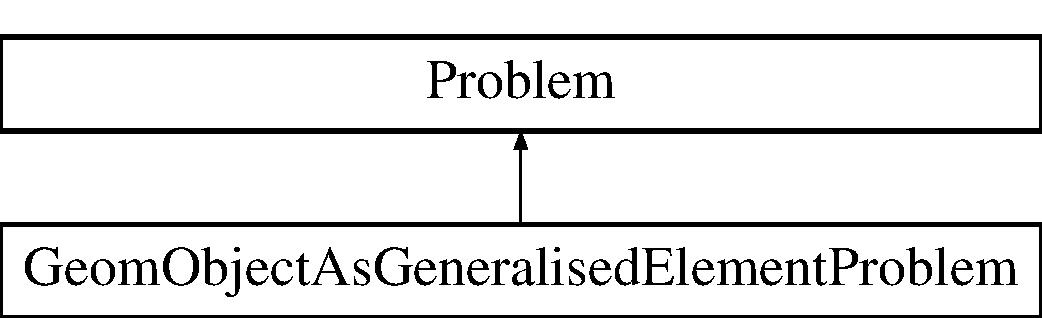
\includegraphics[height=2.000000cm]{classGeomObjectAsGeneralisedElementProblem}
\end{center}
\end{figure}
\subsection*{Public Member Functions}
\begin{DoxyCompactItemize}
\item 
\hyperlink{classGeomObjectAsGeneralisedElementProblem_ad1f15fcb6c055c58d1f71b522f1f7bd6}{Geom\+Object\+As\+Generalised\+Element\+Problem} ()
\begin{DoxyCompactList}\small\item\em Constructor. \end{DoxyCompactList}\item 
void \hyperlink{classGeomObjectAsGeneralisedElementProblem_af396d1789e2552c43e0c68561d88d473}{actions\+\_\+after\+\_\+newton\+\_\+solve} ()
\begin{DoxyCompactList}\small\item\em Update the problem specs after solve (empty) \end{DoxyCompactList}\item 
void \hyperlink{classGeomObjectAsGeneralisedElementProblem_a4ae01862ddbbeeacca1ce7a444e28931}{actions\+\_\+before\+\_\+newton\+\_\+solve} ()
\begin{DoxyCompactList}\small\item\em Update the problem specs before solve (empty) \end{DoxyCompactList}\item 
void \hyperlink{classGeomObjectAsGeneralisedElementProblem_a5092be8e6172d6c9147115bdd485db35}{doc\+\_\+solution} ()
\begin{DoxyCompactList}\small\item\em Doc the solution. \end{DoxyCompactList}\item 
double \& \hyperlink{classGeomObjectAsGeneralisedElementProblem_a5ae799de23742e4c8fa54ee7ae32e679}{load} ()
\begin{DoxyCompactList}\small\item\em Return value of the \char`\"{}load\char`\"{} on the elastically supported ring. \end{DoxyCompactList}\item 
Doc\+Info \& \hyperlink{classGeomObjectAsGeneralisedElementProblem_a4be869d81c0df187d4239a590826f139}{doc\+\_\+info} ()
\begin{DoxyCompactList}\small\item\em Access to Doc\+Info object. \end{DoxyCompactList}\end{DoxyCompactItemize}
\subsection*{Private Attributes}
\begin{DoxyCompactItemize}
\item 
ofstream \hyperlink{classGeomObjectAsGeneralisedElementProblem_ad6261e556a52596ba8904ee902ea6d70}{Trace\+\_\+file}
\begin{DoxyCompactList}\small\item\em Trace file. \end{DoxyCompactList}\item 
Data $\ast$ \hyperlink{classGeomObjectAsGeneralisedElementProblem_ac04469b2dbce010fff3f5b2cf5591bcd}{Load\+\_\+pt}
\begin{DoxyCompactList}\small\item\em Pointer to data item that stores the \char`\"{}load\char`\"{} on the ring. \end{DoxyCompactList}\item 
Doc\+Info \hyperlink{classGeomObjectAsGeneralisedElementProblem_a89a7f5fa555839193166f802d6ff6be2}{Doc\+\_\+info}
\begin{DoxyCompactList}\small\item\em Doc info object. \end{DoxyCompactList}\end{DoxyCompactItemize}


\subsection{Detailed Description}
Problem to demonstrate the use of a Geom\+Object as a Generalised\+Element\+: A geometric object (a Circle) is \char`\"{}upgraded\char`\"{} to a Generalised\+Element. The position of the Circle is determined by a balance of forces, assuming that the Circle is mounted on an elastic spring of specified stiffness and loaded by a vertical \char`\"{}load\char`\"{}. 

Definition at line 56 of file geom\+\_\+object\+\_\+element.\+cc.



\subsection{Constructor \& Destructor Documentation}
\mbox{\Hypertarget{classGeomObjectAsGeneralisedElementProblem_ad1f15fcb6c055c58d1f71b522f1f7bd6}\label{classGeomObjectAsGeneralisedElementProblem_ad1f15fcb6c055c58d1f71b522f1f7bd6}} 
\index{Geom\+Object\+As\+Generalised\+Element\+Problem@{Geom\+Object\+As\+Generalised\+Element\+Problem}!Geom\+Object\+As\+Generalised\+Element\+Problem@{Geom\+Object\+As\+Generalised\+Element\+Problem}}
\index{Geom\+Object\+As\+Generalised\+Element\+Problem@{Geom\+Object\+As\+Generalised\+Element\+Problem}!Geom\+Object\+As\+Generalised\+Element\+Problem@{Geom\+Object\+As\+Generalised\+Element\+Problem}}
\subsubsection{\texorpdfstring{Geom\+Object\+As\+Generalised\+Element\+Problem()}{GeomObjectAsGeneralisedElementProblem()}}
{\footnotesize\ttfamily Geom\+Object\+As\+Generalised\+Element\+Problem\+::\+Geom\+Object\+As\+Generalised\+Element\+Problem (\begin{DoxyParamCaption}{ }\end{DoxyParamCaption})}



Constructor. 



Definition at line 102 of file geom\+\_\+object\+\_\+element.\+cc.



References oomph\+::\+Elastically\+Supported\+Ring\+Element\+::k\+\_\+stiff(), and oomph\+::\+Elastically\+Supported\+Ring\+Element\+::set\+\_\+load\+\_\+pt().



\subsection{Member Function Documentation}
\mbox{\Hypertarget{classGeomObjectAsGeneralisedElementProblem_af396d1789e2552c43e0c68561d88d473}\label{classGeomObjectAsGeneralisedElementProblem_af396d1789e2552c43e0c68561d88d473}} 
\index{Geom\+Object\+As\+Generalised\+Element\+Problem@{Geom\+Object\+As\+Generalised\+Element\+Problem}!actions\+\_\+after\+\_\+newton\+\_\+solve@{actions\+\_\+after\+\_\+newton\+\_\+solve}}
\index{actions\+\_\+after\+\_\+newton\+\_\+solve@{actions\+\_\+after\+\_\+newton\+\_\+solve}!Geom\+Object\+As\+Generalised\+Element\+Problem@{Geom\+Object\+As\+Generalised\+Element\+Problem}}
\subsubsection{\texorpdfstring{actions\+\_\+after\+\_\+newton\+\_\+solve()}{actions\_after\_newton\_solve()}}
{\footnotesize\ttfamily void Geom\+Object\+As\+Generalised\+Element\+Problem\+::actions\+\_\+after\+\_\+newton\+\_\+solve (\begin{DoxyParamCaption}{ }\end{DoxyParamCaption})\hspace{0.3cm}{\ttfamily [inline]}}



Update the problem specs after solve (empty) 



Definition at line 65 of file geom\+\_\+object\+\_\+element.\+cc.

\mbox{\Hypertarget{classGeomObjectAsGeneralisedElementProblem_a4ae01862ddbbeeacca1ce7a444e28931}\label{classGeomObjectAsGeneralisedElementProblem_a4ae01862ddbbeeacca1ce7a444e28931}} 
\index{Geom\+Object\+As\+Generalised\+Element\+Problem@{Geom\+Object\+As\+Generalised\+Element\+Problem}!actions\+\_\+before\+\_\+newton\+\_\+solve@{actions\+\_\+before\+\_\+newton\+\_\+solve}}
\index{actions\+\_\+before\+\_\+newton\+\_\+solve@{actions\+\_\+before\+\_\+newton\+\_\+solve}!Geom\+Object\+As\+Generalised\+Element\+Problem@{Geom\+Object\+As\+Generalised\+Element\+Problem}}
\subsubsection{\texorpdfstring{actions\+\_\+before\+\_\+newton\+\_\+solve()}{actions\_before\_newton\_solve()}}
{\footnotesize\ttfamily void Geom\+Object\+As\+Generalised\+Element\+Problem\+::actions\+\_\+before\+\_\+newton\+\_\+solve (\begin{DoxyParamCaption}{ }\end{DoxyParamCaption})\hspace{0.3cm}{\ttfamily [inline]}}



Update the problem specs before solve (empty) 



Definition at line 68 of file geom\+\_\+object\+\_\+element.\+cc.

\mbox{\Hypertarget{classGeomObjectAsGeneralisedElementProblem_a4be869d81c0df187d4239a590826f139}\label{classGeomObjectAsGeneralisedElementProblem_a4be869d81c0df187d4239a590826f139}} 
\index{Geom\+Object\+As\+Generalised\+Element\+Problem@{Geom\+Object\+As\+Generalised\+Element\+Problem}!doc\+\_\+info@{doc\+\_\+info}}
\index{doc\+\_\+info@{doc\+\_\+info}!Geom\+Object\+As\+Generalised\+Element\+Problem@{Geom\+Object\+As\+Generalised\+Element\+Problem}}
\subsubsection{\texorpdfstring{doc\+\_\+info()}{doc\_info()}}
{\footnotesize\ttfamily Doc\+Info\& Geom\+Object\+As\+Generalised\+Element\+Problem\+::doc\+\_\+info (\begin{DoxyParamCaption}{ }\end{DoxyParamCaption})\hspace{0.3cm}{\ttfamily [inline]}}



Access to Doc\+Info object. 



Definition at line 80 of file geom\+\_\+object\+\_\+element.\+cc.



Referenced by main().

\mbox{\Hypertarget{classGeomObjectAsGeneralisedElementProblem_a5092be8e6172d6c9147115bdd485db35}\label{classGeomObjectAsGeneralisedElementProblem_a5092be8e6172d6c9147115bdd485db35}} 
\index{Geom\+Object\+As\+Generalised\+Element\+Problem@{Geom\+Object\+As\+Generalised\+Element\+Problem}!doc\+\_\+solution@{doc\+\_\+solution}}
\index{doc\+\_\+solution@{doc\+\_\+solution}!Geom\+Object\+As\+Generalised\+Element\+Problem@{Geom\+Object\+As\+Generalised\+Element\+Problem}}
\subsubsection{\texorpdfstring{doc\+\_\+solution()}{doc\_solution()}}
{\footnotesize\ttfamily void Geom\+Object\+As\+Generalised\+Element\+Problem\+::doc\+\_\+solution (\begin{DoxyParamCaption}{ }\end{DoxyParamCaption})}



Doc the solution. 

Doc the solution in tecplot format. 

Definition at line 155 of file geom\+\_\+object\+\_\+element.\+cc.



Referenced by main().

\mbox{\Hypertarget{classGeomObjectAsGeneralisedElementProblem_a5ae799de23742e4c8fa54ee7ae32e679}\label{classGeomObjectAsGeneralisedElementProblem_a5ae799de23742e4c8fa54ee7ae32e679}} 
\index{Geom\+Object\+As\+Generalised\+Element\+Problem@{Geom\+Object\+As\+Generalised\+Element\+Problem}!load@{load}}
\index{load@{load}!Geom\+Object\+As\+Generalised\+Element\+Problem@{Geom\+Object\+As\+Generalised\+Element\+Problem}}
\subsubsection{\texorpdfstring{load()}{load()}}
{\footnotesize\ttfamily double\& Geom\+Object\+As\+Generalised\+Element\+Problem\+::load (\begin{DoxyParamCaption}{ }\end{DoxyParamCaption})\hspace{0.3cm}{\ttfamily [inline]}}



Return value of the \char`\"{}load\char`\"{} on the elastically supported ring. 



Definition at line 74 of file geom\+\_\+object\+\_\+element.\+cc.



Referenced by main().



\subsection{Member Data Documentation}
\mbox{\Hypertarget{classGeomObjectAsGeneralisedElementProblem_a89a7f5fa555839193166f802d6ff6be2}\label{classGeomObjectAsGeneralisedElementProblem_a89a7f5fa555839193166f802d6ff6be2}} 
\index{Geom\+Object\+As\+Generalised\+Element\+Problem@{Geom\+Object\+As\+Generalised\+Element\+Problem}!Doc\+\_\+info@{Doc\+\_\+info}}
\index{Doc\+\_\+info@{Doc\+\_\+info}!Geom\+Object\+As\+Generalised\+Element\+Problem@{Geom\+Object\+As\+Generalised\+Element\+Problem}}
\subsubsection{\texorpdfstring{Doc\+\_\+info}{Doc\_info}}
{\footnotesize\ttfamily Doc\+Info Geom\+Object\+As\+Generalised\+Element\+Problem\+::\+Doc\+\_\+info\hspace{0.3cm}{\ttfamily [private]}}



Doc info object. 



Definition at line 91 of file geom\+\_\+object\+\_\+element.\+cc.

\mbox{\Hypertarget{classGeomObjectAsGeneralisedElementProblem_ac04469b2dbce010fff3f5b2cf5591bcd}\label{classGeomObjectAsGeneralisedElementProblem_ac04469b2dbce010fff3f5b2cf5591bcd}} 
\index{Geom\+Object\+As\+Generalised\+Element\+Problem@{Geom\+Object\+As\+Generalised\+Element\+Problem}!Load\+\_\+pt@{Load\+\_\+pt}}
\index{Load\+\_\+pt@{Load\+\_\+pt}!Geom\+Object\+As\+Generalised\+Element\+Problem@{Geom\+Object\+As\+Generalised\+Element\+Problem}}
\subsubsection{\texorpdfstring{Load\+\_\+pt}{Load\_pt}}
{\footnotesize\ttfamily Data$\ast$ Geom\+Object\+As\+Generalised\+Element\+Problem\+::\+Load\+\_\+pt\hspace{0.3cm}{\ttfamily [private]}}



Pointer to data item that stores the \char`\"{}load\char`\"{} on the ring. 



Definition at line 88 of file geom\+\_\+object\+\_\+element.\+cc.

\mbox{\Hypertarget{classGeomObjectAsGeneralisedElementProblem_ad6261e556a52596ba8904ee902ea6d70}\label{classGeomObjectAsGeneralisedElementProblem_ad6261e556a52596ba8904ee902ea6d70}} 
\index{Geom\+Object\+As\+Generalised\+Element\+Problem@{Geom\+Object\+As\+Generalised\+Element\+Problem}!Trace\+\_\+file@{Trace\+\_\+file}}
\index{Trace\+\_\+file@{Trace\+\_\+file}!Geom\+Object\+As\+Generalised\+Element\+Problem@{Geom\+Object\+As\+Generalised\+Element\+Problem}}
\subsubsection{\texorpdfstring{Trace\+\_\+file}{Trace\_file}}
{\footnotesize\ttfamily ofstream Geom\+Object\+As\+Generalised\+Element\+Problem\+::\+Trace\+\_\+file\hspace{0.3cm}{\ttfamily [private]}}



Trace file. 



Definition at line 85 of file geom\+\_\+object\+\_\+element.\+cc.



The documentation for this class was generated from the following file\+:\begin{DoxyCompactItemize}
\item 
\hyperlink{geom__object__element_8cc}{geom\+\_\+object\+\_\+element.\+cc}\end{DoxyCompactItemize}

\hypertarget{classMyMacroElementNodeUpdateFishMesh}{}\section{My\+Macro\+Element\+Node\+Update\+Fish\+Mesh$<$ E\+L\+E\+M\+E\+NT $>$ Class Template Reference}
\label{classMyMacroElementNodeUpdateFishMesh}\index{My\+Macro\+Element\+Node\+Update\+Fish\+Mesh$<$ E\+L\+E\+M\+E\+N\+T $>$@{My\+Macro\+Element\+Node\+Update\+Fish\+Mesh$<$ E\+L\+E\+M\+E\+N\+T $>$}}


Fish-\/shaped mesh with Macro\+Element-\/based node update.  


Inheritance diagram for My\+Macro\+Element\+Node\+Update\+Fish\+Mesh$<$ E\+L\+E\+M\+E\+NT $>$\+:\begin{figure}[H]
\begin{center}
\leavevmode
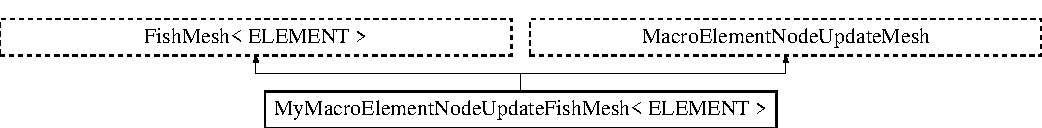
\includegraphics[height=1.723077cm]{classMyMacroElementNodeUpdateFishMesh}
\end{center}
\end{figure}
\subsection*{Public Member Functions}
\begin{DoxyCompactItemize}
\item 
\hyperlink{classMyMacroElementNodeUpdateFishMesh_aa5f87bdc70d79e5361e5c38f6ff0f2ba}{My\+Macro\+Element\+Node\+Update\+Fish\+Mesh} (Geom\+Object $\ast$back\+\_\+pt, Time\+Stepper $\ast$time\+\_\+stepper\+\_\+pt=\&Mesh\+::\+Default\+\_\+\+Time\+Stepper)
\begin{DoxyCompactList}\small\item\em Constructor\+: Pass pointer to Geom\+Object that defines the fish\textquotesingle{}s back and pointer to timestepper (defaults to (Steady) default timestepper defined in the Mesh base class). \end{DoxyCompactList}\item 
virtual \hyperlink{classMyMacroElementNodeUpdateFishMesh_a4498627c037a3f16330ec0c2ff820d1c}{$\sim$\+My\+Macro\+Element\+Node\+Update\+Fish\+Mesh} ()
\begin{DoxyCompactList}\small\item\em Destructor\+: empty. \end{DoxyCompactList}\end{DoxyCompactItemize}


\subsection{Detailed Description}
\subsubsection*{template$<$class E\+L\+E\+M\+E\+NT$>$\newline
class My\+Macro\+Element\+Node\+Update\+Fish\+Mesh$<$ E\+L\+E\+M\+E\+N\+T $>$}

Fish-\/shaped mesh with Macro\+Element-\/based node update. 

Definition at line 92 of file macro\+\_\+element\+\_\+free\+\_\+boundary\+\_\+poisson\+\_\+non\+\_\+ref.\+cc.



\subsection{Constructor \& Destructor Documentation}
\mbox{\Hypertarget{classMyMacroElementNodeUpdateFishMesh_aa5f87bdc70d79e5361e5c38f6ff0f2ba}\label{classMyMacroElementNodeUpdateFishMesh_aa5f87bdc70d79e5361e5c38f6ff0f2ba}} 
\index{My\+Macro\+Element\+Node\+Update\+Fish\+Mesh@{My\+Macro\+Element\+Node\+Update\+Fish\+Mesh}!My\+Macro\+Element\+Node\+Update\+Fish\+Mesh@{My\+Macro\+Element\+Node\+Update\+Fish\+Mesh}}
\index{My\+Macro\+Element\+Node\+Update\+Fish\+Mesh@{My\+Macro\+Element\+Node\+Update\+Fish\+Mesh}!My\+Macro\+Element\+Node\+Update\+Fish\+Mesh@{My\+Macro\+Element\+Node\+Update\+Fish\+Mesh}}
\subsubsection{\texorpdfstring{My\+Macro\+Element\+Node\+Update\+Fish\+Mesh()}{MyMacroElementNodeUpdateFishMesh()}}
{\footnotesize\ttfamily template$<$class E\+L\+E\+M\+E\+NT$>$ \\
\hyperlink{classMyMacroElementNodeUpdateFishMesh}{My\+Macro\+Element\+Node\+Update\+Fish\+Mesh}$<$ E\+L\+E\+M\+E\+NT $>$\+::\hyperlink{classMyMacroElementNodeUpdateFishMesh}{My\+Macro\+Element\+Node\+Update\+Fish\+Mesh} (\begin{DoxyParamCaption}\item[{Geom\+Object $\ast$}]{back\+\_\+pt,  }\item[{Time\+Stepper $\ast$}]{time\+\_\+stepper\+\_\+pt = {\ttfamily \&Mesh\+:\+:Default\+\_\+TimeStepper} }\end{DoxyParamCaption})\hspace{0.3cm}{\ttfamily [inline]}}



Constructor\+: Pass pointer to Geom\+Object that defines the fish\textquotesingle{}s back and pointer to timestepper (defaults to (Steady) default timestepper defined in the Mesh base class). 



Definition at line 103 of file macro\+\_\+element\+\_\+free\+\_\+boundary\+\_\+poisson\+\_\+non\+\_\+ref.\+cc.

\mbox{\Hypertarget{classMyMacroElementNodeUpdateFishMesh_a4498627c037a3f16330ec0c2ff820d1c}\label{classMyMacroElementNodeUpdateFishMesh_a4498627c037a3f16330ec0c2ff820d1c}} 
\index{My\+Macro\+Element\+Node\+Update\+Fish\+Mesh@{My\+Macro\+Element\+Node\+Update\+Fish\+Mesh}!````~My\+Macro\+Element\+Node\+Update\+Fish\+Mesh@{$\sim$\+My\+Macro\+Element\+Node\+Update\+Fish\+Mesh}}
\index{````~My\+Macro\+Element\+Node\+Update\+Fish\+Mesh@{$\sim$\+My\+Macro\+Element\+Node\+Update\+Fish\+Mesh}!My\+Macro\+Element\+Node\+Update\+Fish\+Mesh@{My\+Macro\+Element\+Node\+Update\+Fish\+Mesh}}
\subsubsection{\texorpdfstring{$\sim$\+My\+Macro\+Element\+Node\+Update\+Fish\+Mesh()}{~MyMacroElementNodeUpdateFishMesh()}}
{\footnotesize\ttfamily template$<$class E\+L\+E\+M\+E\+NT$>$ \\
virtual \hyperlink{classMyMacroElementNodeUpdateFishMesh}{My\+Macro\+Element\+Node\+Update\+Fish\+Mesh}$<$ E\+L\+E\+M\+E\+NT $>$\+::$\sim$\hyperlink{classMyMacroElementNodeUpdateFishMesh}{My\+Macro\+Element\+Node\+Update\+Fish\+Mesh} (\begin{DoxyParamCaption}{ }\end{DoxyParamCaption})\hspace{0.3cm}{\ttfamily [inline]}, {\ttfamily [virtual]}}



Destructor\+: empty. 



Definition at line 129 of file macro\+\_\+element\+\_\+free\+\_\+boundary\+\_\+poisson\+\_\+non\+\_\+ref.\+cc.



The documentation for this class was generated from the following file\+:\begin{DoxyCompactItemize}
\item 
\hyperlink{macro__element__free__boundary__poisson__non__ref_8cc}{macro\+\_\+element\+\_\+free\+\_\+boundary\+\_\+poisson\+\_\+non\+\_\+ref.\+cc}\end{DoxyCompactItemize}

\hypertarget{classMyMacroElementNodeUpdateRefineableFishMesh}{}\section{My\+Macro\+Element\+Node\+Update\+Refineable\+Fish\+Mesh$<$ E\+L\+E\+M\+E\+NT $>$ Class Template Reference}
\label{classMyMacroElementNodeUpdateRefineableFishMesh}\index{My\+Macro\+Element\+Node\+Update\+Refineable\+Fish\+Mesh$<$ E\+L\+E\+M\+E\+N\+T $>$@{My\+Macro\+Element\+Node\+Update\+Refineable\+Fish\+Mesh$<$ E\+L\+E\+M\+E\+N\+T $>$}}


Refineable, fish-\/shaped mesh with Macro\+Element-\/based node update.  


Inheritance diagram for My\+Macro\+Element\+Node\+Update\+Refineable\+Fish\+Mesh$<$ E\+L\+E\+M\+E\+NT $>$\+:\begin{figure}[H]
\begin{center}
\leavevmode
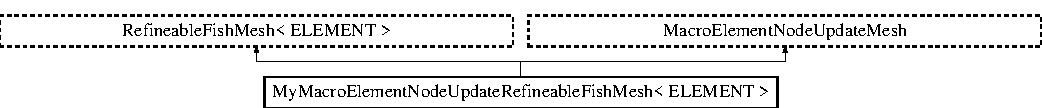
\includegraphics[height=1.454545cm]{classMyMacroElementNodeUpdateRefineableFishMesh}
\end{center}
\end{figure}
\subsection*{Public Member Functions}
\begin{DoxyCompactItemize}
\item 
\hyperlink{classMyMacroElementNodeUpdateRefineableFishMesh_aed0e3ba11f8a2b098ba4e23814135132}{My\+Macro\+Element\+Node\+Update\+Refineable\+Fish\+Mesh} (Geom\+Object $\ast$back\+\_\+pt, Time\+Stepper $\ast$time\+\_\+stepper\+\_\+pt=\&Mesh\+::\+Default\+\_\+\+Time\+Stepper)
\begin{DoxyCompactList}\small\item\em Constructor\+: Pass pointer to Geom\+Object that defines the fish\textquotesingle{}s back and pointer to timestepper (defaults to (Steady) default timestepper defined in the Mesh base class). \end{DoxyCompactList}\item 
virtual \hyperlink{classMyMacroElementNodeUpdateRefineableFishMesh_af125f6a37aedce2fa19309d2908c1b3c}{$\sim$\+My\+Macro\+Element\+Node\+Update\+Refineable\+Fish\+Mesh} ()
\begin{DoxyCompactList}\small\item\em Destructor\+: empty. \end{DoxyCompactList}\end{DoxyCompactItemize}


\subsection{Detailed Description}
\subsubsection*{template$<$class E\+L\+E\+M\+E\+NT$>$\newline
class My\+Macro\+Element\+Node\+Update\+Refineable\+Fish\+Mesh$<$ E\+L\+E\+M\+E\+N\+T $>$}

Refineable, fish-\/shaped mesh with Macro\+Element-\/based node update. 

Definition at line 89 of file macro\+\_\+element\+\_\+free\+\_\+boundary\+\_\+poisson.\+cc.



\subsection{Constructor \& Destructor Documentation}
\mbox{\Hypertarget{classMyMacroElementNodeUpdateRefineableFishMesh_aed0e3ba11f8a2b098ba4e23814135132}\label{classMyMacroElementNodeUpdateRefineableFishMesh_aed0e3ba11f8a2b098ba4e23814135132}} 
\index{My\+Macro\+Element\+Node\+Update\+Refineable\+Fish\+Mesh@{My\+Macro\+Element\+Node\+Update\+Refineable\+Fish\+Mesh}!My\+Macro\+Element\+Node\+Update\+Refineable\+Fish\+Mesh@{My\+Macro\+Element\+Node\+Update\+Refineable\+Fish\+Mesh}}
\index{My\+Macro\+Element\+Node\+Update\+Refineable\+Fish\+Mesh@{My\+Macro\+Element\+Node\+Update\+Refineable\+Fish\+Mesh}!My\+Macro\+Element\+Node\+Update\+Refineable\+Fish\+Mesh@{My\+Macro\+Element\+Node\+Update\+Refineable\+Fish\+Mesh}}
\subsubsection{\texorpdfstring{My\+Macro\+Element\+Node\+Update\+Refineable\+Fish\+Mesh()}{MyMacroElementNodeUpdateRefineableFishMesh()}}
{\footnotesize\ttfamily template$<$class E\+L\+E\+M\+E\+NT$>$ \\
\hyperlink{classMyMacroElementNodeUpdateRefineableFishMesh}{My\+Macro\+Element\+Node\+Update\+Refineable\+Fish\+Mesh}$<$ E\+L\+E\+M\+E\+NT $>$\+::\hyperlink{classMyMacroElementNodeUpdateRefineableFishMesh}{My\+Macro\+Element\+Node\+Update\+Refineable\+Fish\+Mesh} (\begin{DoxyParamCaption}\item[{Geom\+Object $\ast$}]{back\+\_\+pt,  }\item[{Time\+Stepper $\ast$}]{time\+\_\+stepper\+\_\+pt = {\ttfamily \&Mesh\+:\+:Default\+\_\+TimeStepper} }\end{DoxyParamCaption})\hspace{0.3cm}{\ttfamily [inline]}}



Constructor\+: Pass pointer to Geom\+Object that defines the fish\textquotesingle{}s back and pointer to timestepper (defaults to (Steady) default timestepper defined in the Mesh base class). 



Definition at line 100 of file macro\+\_\+element\+\_\+free\+\_\+boundary\+\_\+poisson.\+cc.

\mbox{\Hypertarget{classMyMacroElementNodeUpdateRefineableFishMesh_af125f6a37aedce2fa19309d2908c1b3c}\label{classMyMacroElementNodeUpdateRefineableFishMesh_af125f6a37aedce2fa19309d2908c1b3c}} 
\index{My\+Macro\+Element\+Node\+Update\+Refineable\+Fish\+Mesh@{My\+Macro\+Element\+Node\+Update\+Refineable\+Fish\+Mesh}!````~My\+Macro\+Element\+Node\+Update\+Refineable\+Fish\+Mesh@{$\sim$\+My\+Macro\+Element\+Node\+Update\+Refineable\+Fish\+Mesh}}
\index{````~My\+Macro\+Element\+Node\+Update\+Refineable\+Fish\+Mesh@{$\sim$\+My\+Macro\+Element\+Node\+Update\+Refineable\+Fish\+Mesh}!My\+Macro\+Element\+Node\+Update\+Refineable\+Fish\+Mesh@{My\+Macro\+Element\+Node\+Update\+Refineable\+Fish\+Mesh}}
\subsubsection{\texorpdfstring{$\sim$\+My\+Macro\+Element\+Node\+Update\+Refineable\+Fish\+Mesh()}{~MyMacroElementNodeUpdateRefineableFishMesh()}}
{\footnotesize\ttfamily template$<$class E\+L\+E\+M\+E\+NT$>$ \\
virtual \hyperlink{classMyMacroElementNodeUpdateRefineableFishMesh}{My\+Macro\+Element\+Node\+Update\+Refineable\+Fish\+Mesh}$<$ E\+L\+E\+M\+E\+NT $>$\+::$\sim$\hyperlink{classMyMacroElementNodeUpdateRefineableFishMesh}{My\+Macro\+Element\+Node\+Update\+Refineable\+Fish\+Mesh} (\begin{DoxyParamCaption}{ }\end{DoxyParamCaption})\hspace{0.3cm}{\ttfamily [inline]}, {\ttfamily [virtual]}}



Destructor\+: empty. 



Definition at line 126 of file macro\+\_\+element\+\_\+free\+\_\+boundary\+\_\+poisson.\+cc.



The documentation for this class was generated from the following file\+:\begin{DoxyCompactItemize}
\item 
\hyperlink{macro__element__free__boundary__poisson_8cc}{macro\+\_\+element\+\_\+free\+\_\+boundary\+\_\+poisson.\+cc}\end{DoxyCompactItemize}

\hypertarget{classRefineableFishPoissonProblem}{}\section{Refineable\+Fish\+Poisson\+Problem$<$ E\+L\+E\+M\+E\+NT $>$ Class Template Reference}
\label{classRefineableFishPoissonProblem}\index{Refineable\+Fish\+Poisson\+Problem$<$ E\+L\+E\+M\+E\+N\+T $>$@{Refineable\+Fish\+Poisson\+Problem$<$ E\+L\+E\+M\+E\+N\+T $>$}}
Inheritance diagram for Refineable\+Fish\+Poisson\+Problem$<$ E\+L\+E\+M\+E\+NT $>$\+:\begin{figure}[H]
\begin{center}
\leavevmode
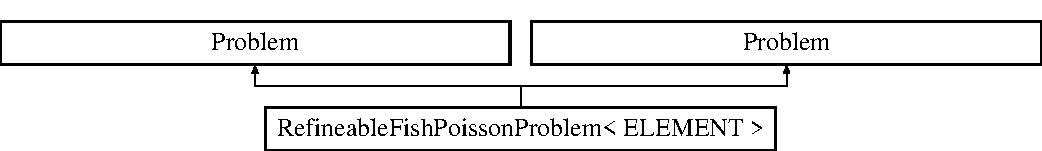
\includegraphics[height=2.000000cm]{classRefineableFishPoissonProblem}
\end{center}
\end{figure}
\subsection*{Public Member Functions}
\begin{DoxyCompactItemize}
\item 
\hyperlink{classRefineableFishPoissonProblem_a2585d906fab348e09bfb9b4c111ac161}{Refineable\+Fish\+Poisson\+Problem} (const bool \&fix\+\_\+position, const string \&directory\+\_\+name, const unsigned \&i\+\_\+case)
\begin{DoxyCompactList}\small\item\em Constructor\+: Bool flag specifies if position of fish back is prescribed or computed from the coupled problem. String specifies output directory. \end{DoxyCompactList}\item 
virtual \hyperlink{classRefineableFishPoissonProblem_a7039a3409520850908940927b91af9ab}{$\sim$\+Refineable\+Fish\+Poisson\+Problem} ()
\begin{DoxyCompactList}\small\item\em Destructor. \end{DoxyCompactList}\item 
void \hyperlink{classRefineableFishPoissonProblem_a8d8fb7ef1c571c57c02073edab4a7759}{actions\+\_\+before\+\_\+newton\+\_\+convergence\+\_\+check} ()
\begin{DoxyCompactList}\small\item\em Update after Newton step\+: Update mesh in response to possible changes in the wall shape. \end{DoxyCompactList}\item 
void \hyperlink{classRefineableFishPoissonProblem_a7f6c356f7c8bd0130de957297e999f40}{actions\+\_\+after\+\_\+newton\+\_\+solve} ()
\begin{DoxyCompactList}\small\item\em Update the problem specs after solve (empty) \end{DoxyCompactList}\item 
void \hyperlink{classRefineableFishPoissonProblem_a58098181f3b88c2fc65f24fb15c1a529}{actions\+\_\+before\+\_\+newton\+\_\+solve} ()
\begin{DoxyCompactList}\small\item\em Update the problem specs before solve\+: Update mesh. \end{DoxyCompactList}\item 
Algebraic\+Refineable\+Fish\+Mesh$<$ E\+L\+E\+M\+E\+NT $>$ $\ast$ \hyperlink{classRefineableFishPoissonProblem_a6f25d5110e5262e66e2900da051567a6}{fish\+\_\+mesh\+\_\+pt} ()
\item 
double \& \hyperlink{classRefineableFishPoissonProblem_a20702e8945d442c9597348b550da14e4}{load} ()
\begin{DoxyCompactList}\small\item\em Return value of the \char`\"{}load\char`\"{} on the elastically supported ring. \end{DoxyCompactList}\item 
double \& \hyperlink{classRefineableFishPoissonProblem_a152227cc825ddea07cb06c2791f5995b}{y\+\_\+c} ()
\begin{DoxyCompactList}\small\item\em Return value of the vertical displacement of the ring that represents the fish\textquotesingle{}s back. \end{DoxyCompactList}\item 
void \hyperlink{classRefineableFishPoissonProblem_a6db25ff0bd3014aa531d9f0e8b385beb}{doc\+\_\+solution} ()
\begin{DoxyCompactList}\small\item\em Doc the solution. \end{DoxyCompactList}\item 
Doc\+Info \& \hyperlink{classRefineableFishPoissonProblem_a093f5963e63746843c33ca444a205333}{doc\+\_\+info} ()
\begin{DoxyCompactList}\small\item\em Access to Doc\+Info object. \end{DoxyCompactList}\item 
\hyperlink{classRefineableFishPoissonProblem_a0211667b09b7da71184de2524609701f}{Refineable\+Fish\+Poisson\+Problem} (bool fix\+\_\+position, string directory\+\_\+name)
\begin{DoxyCompactList}\small\item\em Constructor\+: Bool flag specifies if position of fish back is prescribed or computed from the coupled problem. String specifies output directory. \end{DoxyCompactList}\item 
virtual \hyperlink{classRefineableFishPoissonProblem_a4a5e7c5f264364211ad641353933c222}{$\sim$\+Refineable\+Fish\+Poisson\+Problem} ()
\begin{DoxyCompactList}\small\item\em Destructor. \end{DoxyCompactList}\item 
void \hyperlink{classRefineableFishPoissonProblem_a8d8fb7ef1c571c57c02073edab4a7759}{actions\+\_\+before\+\_\+newton\+\_\+convergence\+\_\+check} ()
\begin{DoxyCompactList}\small\item\em Update after Newton step\+: Update in response to possible changes in the wall shape. \end{DoxyCompactList}\item 
void \hyperlink{classRefineableFishPoissonProblem_a58098181f3b88c2fc65f24fb15c1a529}{actions\+\_\+before\+\_\+newton\+\_\+solve} ()
\begin{DoxyCompactList}\small\item\em Update the problem specs before solve\+: Update nodal positions. \end{DoxyCompactList}\item 
void \hyperlink{classRefineableFishPoissonProblem_a7f6c356f7c8bd0130de957297e999f40}{actions\+\_\+after\+\_\+newton\+\_\+solve} ()
\begin{DoxyCompactList}\small\item\em Update the problem specs after solve (empty) \end{DoxyCompactList}\item 
Macro\+Element\+Node\+Update\+Refineable\+Fish\+Mesh$<$ E\+L\+E\+M\+E\+NT $>$ $\ast$ \hyperlink{classRefineableFishPoissonProblem_ab472201df89d71930157fbc45b8eaa54}{fish\+\_\+mesh\+\_\+pt} ()
\item 
double \& \hyperlink{classRefineableFishPoissonProblem_a20702e8945d442c9597348b550da14e4}{load} ()
\begin{DoxyCompactList}\small\item\em Return value of the \char`\"{}load\char`\"{} on the elastically supported ring that represents the fish\textquotesingle{}s back. \end{DoxyCompactList}\item 
double \& \hyperlink{classRefineableFishPoissonProblem_a152227cc825ddea07cb06c2791f5995b}{y\+\_\+c} ()
\begin{DoxyCompactList}\small\item\em Return value of the vertical displacement of the ring that represents the fish\textquotesingle{}s back. \end{DoxyCompactList}\item 
void \hyperlink{classRefineableFishPoissonProblem_a6db25ff0bd3014aa531d9f0e8b385beb}{doc\+\_\+solution} ()
\begin{DoxyCompactList}\small\item\em Doc the solution. \end{DoxyCompactList}\item 
Doc\+Info \& \hyperlink{classRefineableFishPoissonProblem_a093f5963e63746843c33ca444a205333}{doc\+\_\+info} ()
\begin{DoxyCompactList}\small\item\em Access to Doc\+Info object. \end{DoxyCompactList}\end{DoxyCompactItemize}
\subsection*{Private Member Functions}
\begin{DoxyCompactItemize}
\item 
void \hyperlink{classRefineableFishPoissonProblem_a122cddf55249eaf0ee813818ff101fb4}{set\+\_\+shape\+\_\+deriv\+\_\+method} ()
\begin{DoxyCompactList}\small\item\em Helper fct to set method for evaluation of shape derivs. \end{DoxyCompactList}\end{DoxyCompactItemize}
\subsection*{Private Attributes}
\begin{DoxyCompactItemize}
\item 
Node $\ast$ \hyperlink{classRefineableFishPoissonProblem_a5dce47aa14fdbc33d8a865f4f4b1e1ea}{Doc\+\_\+node\+\_\+pt}
\begin{DoxyCompactList}\small\item\em Node at which the solution of the Poisson equation is documented. \end{DoxyCompactList}\item 
ofstream \hyperlink{classRefineableFishPoissonProblem_aa358e2b0fa91780bdca32ae4676717ff}{Trace\+\_\+file}
\begin{DoxyCompactList}\small\item\em Trace file. \end{DoxyCompactList}\item 
Algebraic\+Refineable\+Fish\+Mesh$<$ E\+L\+E\+M\+E\+NT $>$ $\ast$ \hyperlink{classRefineableFishPoissonProblem_af915f09b6e4ae2f4ded2ad1a25ed7f01}{Fish\+\_\+mesh\+\_\+pt}
\begin{DoxyCompactList}\small\item\em Pointer to fish mesh. \end{DoxyCompactList}\item 
Mesh $\ast$ \hyperlink{classRefineableFishPoissonProblem_ac0f6f58b393715961214d98e11dfad57}{Fish\+\_\+back\+\_\+mesh\+\_\+pt}
\item 
Data $\ast$ \hyperlink{classRefineableFishPoissonProblem_a9a9ce82a4308be486701578134d06210}{Load\+\_\+pt}
\begin{DoxyCompactList}\small\item\em Pointer to data item that stores the \char`\"{}load\char`\"{} on the fish back. \end{DoxyCompactList}\item 
bool \hyperlink{classRefineableFishPoissonProblem_a51c10ea7cbf4ab61fd953f011f72a1c4}{Fix\+\_\+position}
\begin{DoxyCompactList}\small\item\em Is the position of the fish back prescribed? \end{DoxyCompactList}\item 
Doc\+Info \hyperlink{classRefineableFishPoissonProblem_ad6d382f1d38425323627f34e0559b28f}{Doc\+\_\+info}
\begin{DoxyCompactList}\small\item\em Doc info object. \end{DoxyCompactList}\item 
unsigned \hyperlink{classRefineableFishPoissonProblem_af6f409d7fe711ad809d9e784d98ca036}{Case\+\_\+id}
\begin{DoxyCompactList}\small\item\em Case id. \end{DoxyCompactList}\item 
Macro\+Element\+Node\+Update\+Refineable\+Fish\+Mesh$<$ E\+L\+E\+M\+E\+NT $>$ $\ast$ \hyperlink{classRefineableFishPoissonProblem_a769ab4e05f6962a7c8fc85f03a261916}{Fish\+\_\+mesh\+\_\+pt}
\begin{DoxyCompactList}\small\item\em Pointer to fish mesh. \end{DoxyCompactList}\end{DoxyCompactItemize}


\subsection{Detailed Description}
\subsubsection*{template$<$class E\+L\+E\+M\+E\+NT$>$\newline
class Refineable\+Fish\+Poisson\+Problem$<$ E\+L\+E\+M\+E\+N\+T $>$}

Refineable Poisson problem in deformable fish-\/shaped domain. Template parameter identify the elements.

Refineable Poisson problem in deformable fish-\/shaped domain. Template parameter identifies the element. 

Definition at line 84 of file algebraic\+\_\+free\+\_\+boundary\+\_\+poisson.\+cc.



\subsection{Constructor \& Destructor Documentation}
\mbox{\Hypertarget{classRefineableFishPoissonProblem_a2585d906fab348e09bfb9b4c111ac161}\label{classRefineableFishPoissonProblem_a2585d906fab348e09bfb9b4c111ac161}} 
\index{Refineable\+Fish\+Poisson\+Problem@{Refineable\+Fish\+Poisson\+Problem}!Refineable\+Fish\+Poisson\+Problem@{Refineable\+Fish\+Poisson\+Problem}}
\index{Refineable\+Fish\+Poisson\+Problem@{Refineable\+Fish\+Poisson\+Problem}!Refineable\+Fish\+Poisson\+Problem@{Refineable\+Fish\+Poisson\+Problem}}
\subsubsection{\texorpdfstring{Refineable\+Fish\+Poisson\+Problem()}{RefineableFishPoissonProblem()}\hspace{0.1cm}{\footnotesize\ttfamily [1/2]}}
{\footnotesize\ttfamily template$<$class E\+L\+E\+M\+E\+NT $>$ \\
\hyperlink{classRefineableFishPoissonProblem}{Refineable\+Fish\+Poisson\+Problem}$<$ E\+L\+E\+M\+E\+NT $>$\+::\hyperlink{classRefineableFishPoissonProblem}{Refineable\+Fish\+Poisson\+Problem} (\begin{DoxyParamCaption}\item[{const bool \&}]{fix\+\_\+position,  }\item[{const string \&}]{directory\+\_\+name,  }\item[{const unsigned \&}]{i\+\_\+case }\end{DoxyParamCaption})}



Constructor\+: Bool flag specifies if position of fish back is prescribed or computed from the coupled problem. String specifies output directory. 

Constructor for adaptive Poisson problem in deformable fish-\/shaped domain. Pass flag if position of fish back is fixed, and the output directory. Loop over elements and set pointers to source function 

Definition at line 244 of file algebraic\+\_\+free\+\_\+boundary\+\_\+poisson.\+cc.



References Refineable\+Fish\+Poisson\+Problem$<$ E\+L\+E\+M\+E\+N\+T $>$\+::\+Doc\+\_\+info, Refineable\+Fish\+Poisson\+Problem$<$ E\+L\+E\+M\+E\+N\+T $>$\+::\+Doc\+\_\+node\+\_\+pt, Refineable\+Fish\+Poisson\+Problem$<$ E\+L\+E\+M\+E\+N\+T $>$\+::\+Fish\+\_\+back\+\_\+mesh\+\_\+pt, Refineable\+Fish\+Poisson\+Problem$<$ E\+L\+E\+M\+E\+N\+T $>$\+::fish\+\_\+mesh\+\_\+pt(), Refineable\+Fish\+Poisson\+Problem$<$ E\+L\+E\+M\+E\+N\+T $>$\+::\+Fish\+\_\+mesh\+\_\+pt, Refineable\+Fish\+Poisson\+Problem$<$ E\+L\+E\+M\+E\+N\+T $>$\+::\+Fix\+\_\+position, Const\+Source\+For\+Poisson\+::get\+\_\+source(), Refineable\+Fish\+Poisson\+Problem$<$ E\+L\+E\+M\+E\+N\+T $>$\+::\+Load\+\_\+pt, Refineable\+Fish\+Poisson\+Problem$<$ E\+L\+E\+M\+E\+N\+T $>$\+::set\+\_\+shape\+\_\+deriv\+\_\+method(), Refineable\+Fish\+Poisson\+Problem$<$ E\+L\+E\+M\+E\+N\+T $>$\+::\+Trace\+\_\+file, and Refineable\+Fish\+Poisson\+Problem$<$ E\+L\+E\+M\+E\+N\+T $>$\+::y\+\_\+c().

\mbox{\Hypertarget{classRefineableFishPoissonProblem_a7039a3409520850908940927b91af9ab}\label{classRefineableFishPoissonProblem_a7039a3409520850908940927b91af9ab}} 
\index{Refineable\+Fish\+Poisson\+Problem@{Refineable\+Fish\+Poisson\+Problem}!````~Refineable\+Fish\+Poisson\+Problem@{$\sim$\+Refineable\+Fish\+Poisson\+Problem}}
\index{````~Refineable\+Fish\+Poisson\+Problem@{$\sim$\+Refineable\+Fish\+Poisson\+Problem}!Refineable\+Fish\+Poisson\+Problem@{Refineable\+Fish\+Poisson\+Problem}}
\subsubsection{\texorpdfstring{$\sim$\+Refineable\+Fish\+Poisson\+Problem()}{~RefineableFishPoissonProblem()}\hspace{0.1cm}{\footnotesize\ttfamily [1/2]}}
{\footnotesize\ttfamily template$<$class E\+L\+E\+M\+E\+NT $>$ \\
\hyperlink{classRefineableFishPoissonProblem}{Refineable\+Fish\+Poisson\+Problem}$<$ E\+L\+E\+M\+E\+NT $>$\+::$\sim$\hyperlink{classRefineableFishPoissonProblem}{Refineable\+Fish\+Poisson\+Problem} (\begin{DoxyParamCaption}{ }\end{DoxyParamCaption})\hspace{0.3cm}{\ttfamily [virtual]}}



Destructor. 

Destructor for Poisson problem in deformable fish-\/shaped domain. 

Definition at line 394 of file algebraic\+\_\+free\+\_\+boundary\+\_\+poisson.\+cc.



References Refineable\+Fish\+Poisson\+Problem$<$ E\+L\+E\+M\+E\+N\+T $>$\+::\+Trace\+\_\+file.



Referenced by Refineable\+Fish\+Poisson\+Problem$<$ E\+L\+E\+M\+E\+N\+T $>$\+::\+Refineable\+Fish\+Poisson\+Problem().

\mbox{\Hypertarget{classRefineableFishPoissonProblem_a0211667b09b7da71184de2524609701f}\label{classRefineableFishPoissonProblem_a0211667b09b7da71184de2524609701f}} 
\index{Refineable\+Fish\+Poisson\+Problem@{Refineable\+Fish\+Poisson\+Problem}!Refineable\+Fish\+Poisson\+Problem@{Refineable\+Fish\+Poisson\+Problem}}
\index{Refineable\+Fish\+Poisson\+Problem@{Refineable\+Fish\+Poisson\+Problem}!Refineable\+Fish\+Poisson\+Problem@{Refineable\+Fish\+Poisson\+Problem}}
\subsubsection{\texorpdfstring{Refineable\+Fish\+Poisson\+Problem()}{RefineableFishPoissonProblem()}\hspace{0.1cm}{\footnotesize\ttfamily [2/2]}}
{\footnotesize\ttfamily template$<$class E\+L\+E\+M\+E\+NT $>$ \\
\hyperlink{classRefineableFishPoissonProblem}{Refineable\+Fish\+Poisson\+Problem}$<$ E\+L\+E\+M\+E\+NT $>$\+::\hyperlink{classRefineableFishPoissonProblem}{Refineable\+Fish\+Poisson\+Problem} (\begin{DoxyParamCaption}\item[{bool}]{fix\+\_\+position,  }\item[{string}]{directory\+\_\+name }\end{DoxyParamCaption})}



Constructor\+: Bool flag specifies if position of fish back is prescribed or computed from the coupled problem. String specifies output directory. 

Constructor for adaptive Poisson problem in deformable fish-\/shaped domain. Pass flag if position of fish back is fixed, and the output directory. Loop over elements and set pointers to source function 

Definition at line 184 of file old\+\_\+for\+\_\+doc.\+cc.



References Refineable\+Fish\+Poisson\+Problem$<$ E\+L\+E\+M\+E\+N\+T $>$\+::\+Doc\+\_\+info, Refineable\+Fish\+Poisson\+Problem$<$ E\+L\+E\+M\+E\+N\+T $>$\+::\+Doc\+\_\+node\+\_\+pt, Refineable\+Fish\+Poisson\+Problem$<$ E\+L\+E\+M\+E\+N\+T $>$\+::doc\+\_\+solution(), Refineable\+Fish\+Poisson\+Problem$<$ E\+L\+E\+M\+E\+N\+T $>$\+::\+Fish\+\_\+back\+\_\+mesh\+\_\+pt, Refineable\+Fish\+Poisson\+Problem$<$ E\+L\+E\+M\+E\+N\+T $>$\+::fish\+\_\+mesh\+\_\+pt(), Refineable\+Fish\+Poisson\+Problem$<$ E\+L\+E\+M\+E\+N\+T $>$\+::\+Fish\+\_\+mesh\+\_\+pt, Refineable\+Fish\+Poisson\+Problem$<$ E\+L\+E\+M\+E\+N\+T $>$\+::\+Fix\+\_\+position, Const\+Source\+For\+Poisson\+::get\+\_\+source(), Refineable\+Fish\+Poisson\+Problem$<$ E\+L\+E\+M\+E\+N\+T $>$\+::load(), Refineable\+Fish\+Poisson\+Problem$<$ E\+L\+E\+M\+E\+N\+T $>$\+::\+Load\+\_\+pt, Refineable\+Fish\+Poisson\+Problem$<$ E\+L\+E\+M\+E\+N\+T $>$\+::\+Trace\+\_\+file, Refineable\+Fish\+Poisson\+Problem$<$ E\+L\+E\+M\+E\+N\+T $>$\+::y\+\_\+c(), and Refineable\+Fish\+Poisson\+Problem$<$ E\+L\+E\+M\+E\+N\+T $>$\+::$\sim$\+Refineable\+Fish\+Poisson\+Problem().

\mbox{\Hypertarget{classRefineableFishPoissonProblem_a4a5e7c5f264364211ad641353933c222}\label{classRefineableFishPoissonProblem_a4a5e7c5f264364211ad641353933c222}} 
\index{Refineable\+Fish\+Poisson\+Problem@{Refineable\+Fish\+Poisson\+Problem}!````~Refineable\+Fish\+Poisson\+Problem@{$\sim$\+Refineable\+Fish\+Poisson\+Problem}}
\index{````~Refineable\+Fish\+Poisson\+Problem@{$\sim$\+Refineable\+Fish\+Poisson\+Problem}!Refineable\+Fish\+Poisson\+Problem@{Refineable\+Fish\+Poisson\+Problem}}
\subsubsection{\texorpdfstring{$\sim$\+Refineable\+Fish\+Poisson\+Problem()}{~RefineableFishPoissonProblem()}\hspace{0.1cm}{\footnotesize\ttfamily [2/2]}}
{\footnotesize\ttfamily template$<$class E\+L\+E\+M\+E\+NT$>$ \\
virtual \hyperlink{classRefineableFishPoissonProblem}{Refineable\+Fish\+Poisson\+Problem}$<$ E\+L\+E\+M\+E\+NT $>$\+::$\sim$\hyperlink{classRefineableFishPoissonProblem}{Refineable\+Fish\+Poisson\+Problem} (\begin{DoxyParamCaption}{ }\end{DoxyParamCaption})\hspace{0.3cm}{\ttfamily [virtual]}}



Destructor. 



\subsection{Member Function Documentation}
\mbox{\Hypertarget{classRefineableFishPoissonProblem_a7f6c356f7c8bd0130de957297e999f40}\label{classRefineableFishPoissonProblem_a7f6c356f7c8bd0130de957297e999f40}} 
\index{Refineable\+Fish\+Poisson\+Problem@{Refineable\+Fish\+Poisson\+Problem}!actions\+\_\+after\+\_\+newton\+\_\+solve@{actions\+\_\+after\+\_\+newton\+\_\+solve}}
\index{actions\+\_\+after\+\_\+newton\+\_\+solve@{actions\+\_\+after\+\_\+newton\+\_\+solve}!Refineable\+Fish\+Poisson\+Problem@{Refineable\+Fish\+Poisson\+Problem}}
\subsubsection{\texorpdfstring{actions\+\_\+after\+\_\+newton\+\_\+solve()}{actions\_after\_newton\_solve()}\hspace{0.1cm}{\footnotesize\ttfamily [1/2]}}
{\footnotesize\ttfamily template$<$class E\+L\+E\+M\+E\+NT$>$ \\
void \hyperlink{classRefineableFishPoissonProblem}{Refineable\+Fish\+Poisson\+Problem}$<$ E\+L\+E\+M\+E\+NT $>$\+::actions\+\_\+after\+\_\+newton\+\_\+solve (\begin{DoxyParamCaption}{ }\end{DoxyParamCaption})\hspace{0.3cm}{\ttfamily [inline]}}



Update the problem specs after solve (empty) 



Definition at line 107 of file algebraic\+\_\+free\+\_\+boundary\+\_\+poisson.\+cc.

\mbox{\Hypertarget{classRefineableFishPoissonProblem_a7f6c356f7c8bd0130de957297e999f40}\label{classRefineableFishPoissonProblem_a7f6c356f7c8bd0130de957297e999f40}} 
\index{Refineable\+Fish\+Poisson\+Problem@{Refineable\+Fish\+Poisson\+Problem}!actions\+\_\+after\+\_\+newton\+\_\+solve@{actions\+\_\+after\+\_\+newton\+\_\+solve}}
\index{actions\+\_\+after\+\_\+newton\+\_\+solve@{actions\+\_\+after\+\_\+newton\+\_\+solve}!Refineable\+Fish\+Poisson\+Problem@{Refineable\+Fish\+Poisson\+Problem}}
\subsubsection{\texorpdfstring{actions\+\_\+after\+\_\+newton\+\_\+solve()}{actions\_after\_newton\_solve()}\hspace{0.1cm}{\footnotesize\ttfamily [2/2]}}
{\footnotesize\ttfamily template$<$class E\+L\+E\+M\+E\+NT$>$ \\
void \hyperlink{classRefineableFishPoissonProblem}{Refineable\+Fish\+Poisson\+Problem}$<$ E\+L\+E\+M\+E\+NT $>$\+::actions\+\_\+after\+\_\+newton\+\_\+solve (\begin{DoxyParamCaption}{ }\end{DoxyParamCaption})\hspace{0.3cm}{\ttfamily [inline]}}



Update the problem specs after solve (empty) 



Definition at line 117 of file old\+\_\+for\+\_\+doc.\+cc.

\mbox{\Hypertarget{classRefineableFishPoissonProblem_a8d8fb7ef1c571c57c02073edab4a7759}\label{classRefineableFishPoissonProblem_a8d8fb7ef1c571c57c02073edab4a7759}} 
\index{Refineable\+Fish\+Poisson\+Problem@{Refineable\+Fish\+Poisson\+Problem}!actions\+\_\+before\+\_\+newton\+\_\+convergence\+\_\+check@{actions\+\_\+before\+\_\+newton\+\_\+convergence\+\_\+check}}
\index{actions\+\_\+before\+\_\+newton\+\_\+convergence\+\_\+check@{actions\+\_\+before\+\_\+newton\+\_\+convergence\+\_\+check}!Refineable\+Fish\+Poisson\+Problem@{Refineable\+Fish\+Poisson\+Problem}}
\subsubsection{\texorpdfstring{actions\+\_\+before\+\_\+newton\+\_\+convergence\+\_\+check()}{actions\_before\_newton\_convergence\_check()}\hspace{0.1cm}{\footnotesize\ttfamily [1/2]}}
{\footnotesize\ttfamily template$<$class E\+L\+E\+M\+E\+NT$>$ \\
void \hyperlink{classRefineableFishPoissonProblem}{Refineable\+Fish\+Poisson\+Problem}$<$ E\+L\+E\+M\+E\+NT $>$\+::actions\+\_\+before\+\_\+newton\+\_\+convergence\+\_\+check (\begin{DoxyParamCaption}{ }\end{DoxyParamCaption})\hspace{0.3cm}{\ttfamily [inline]}}



Update after Newton step\+: Update mesh in response to possible changes in the wall shape. 



Definition at line 101 of file algebraic\+\_\+free\+\_\+boundary\+\_\+poisson.\+cc.

\mbox{\Hypertarget{classRefineableFishPoissonProblem_a8d8fb7ef1c571c57c02073edab4a7759}\label{classRefineableFishPoissonProblem_a8d8fb7ef1c571c57c02073edab4a7759}} 
\index{Refineable\+Fish\+Poisson\+Problem@{Refineable\+Fish\+Poisson\+Problem}!actions\+\_\+before\+\_\+newton\+\_\+convergence\+\_\+check@{actions\+\_\+before\+\_\+newton\+\_\+convergence\+\_\+check}}
\index{actions\+\_\+before\+\_\+newton\+\_\+convergence\+\_\+check@{actions\+\_\+before\+\_\+newton\+\_\+convergence\+\_\+check}!Refineable\+Fish\+Poisson\+Problem@{Refineable\+Fish\+Poisson\+Problem}}
\subsubsection{\texorpdfstring{actions\+\_\+before\+\_\+newton\+\_\+convergence\+\_\+check()}{actions\_before\_newton\_convergence\_check()}\hspace{0.1cm}{\footnotesize\ttfamily [2/2]}}
{\footnotesize\ttfamily template$<$class E\+L\+E\+M\+E\+NT$>$ \\
void \hyperlink{classRefineableFishPoissonProblem}{Refineable\+Fish\+Poisson\+Problem}$<$ E\+L\+E\+M\+E\+NT $>$\+::actions\+\_\+before\+\_\+newton\+\_\+convergence\+\_\+check (\begin{DoxyParamCaption}{ }\end{DoxyParamCaption})\hspace{0.3cm}{\ttfamily [inline]}}



Update after Newton step\+: Update in response to possible changes in the wall shape. 



Definition at line 104 of file old\+\_\+for\+\_\+doc.\+cc.

\mbox{\Hypertarget{classRefineableFishPoissonProblem_a58098181f3b88c2fc65f24fb15c1a529}\label{classRefineableFishPoissonProblem_a58098181f3b88c2fc65f24fb15c1a529}} 
\index{Refineable\+Fish\+Poisson\+Problem@{Refineable\+Fish\+Poisson\+Problem}!actions\+\_\+before\+\_\+newton\+\_\+solve@{actions\+\_\+before\+\_\+newton\+\_\+solve}}
\index{actions\+\_\+before\+\_\+newton\+\_\+solve@{actions\+\_\+before\+\_\+newton\+\_\+solve}!Refineable\+Fish\+Poisson\+Problem@{Refineable\+Fish\+Poisson\+Problem}}
\subsubsection{\texorpdfstring{actions\+\_\+before\+\_\+newton\+\_\+solve()}{actions\_before\_newton\_solve()}\hspace{0.1cm}{\footnotesize\ttfamily [1/2]}}
{\footnotesize\ttfamily template$<$class E\+L\+E\+M\+E\+NT$>$ \\
void \hyperlink{classRefineableFishPoissonProblem}{Refineable\+Fish\+Poisson\+Problem}$<$ E\+L\+E\+M\+E\+NT $>$\+::actions\+\_\+before\+\_\+newton\+\_\+solve (\begin{DoxyParamCaption}{ }\end{DoxyParamCaption})\hspace{0.3cm}{\ttfamily [inline]}}



Update the problem specs before solve\+: Update mesh. 



Definition at line 110 of file algebraic\+\_\+free\+\_\+boundary\+\_\+poisson.\+cc.

\mbox{\Hypertarget{classRefineableFishPoissonProblem_a58098181f3b88c2fc65f24fb15c1a529}\label{classRefineableFishPoissonProblem_a58098181f3b88c2fc65f24fb15c1a529}} 
\index{Refineable\+Fish\+Poisson\+Problem@{Refineable\+Fish\+Poisson\+Problem}!actions\+\_\+before\+\_\+newton\+\_\+solve@{actions\+\_\+before\+\_\+newton\+\_\+solve}}
\index{actions\+\_\+before\+\_\+newton\+\_\+solve@{actions\+\_\+before\+\_\+newton\+\_\+solve}!Refineable\+Fish\+Poisson\+Problem@{Refineable\+Fish\+Poisson\+Problem}}
\subsubsection{\texorpdfstring{actions\+\_\+before\+\_\+newton\+\_\+solve()}{actions\_before\_newton\_solve()}\hspace{0.1cm}{\footnotesize\ttfamily [2/2]}}
{\footnotesize\ttfamily template$<$class E\+L\+E\+M\+E\+NT$>$ \\
void \hyperlink{classRefineableFishPoissonProblem}{Refineable\+Fish\+Poisson\+Problem}$<$ E\+L\+E\+M\+E\+NT $>$\+::actions\+\_\+before\+\_\+newton\+\_\+solve (\begin{DoxyParamCaption}{ }\end{DoxyParamCaption})\hspace{0.3cm}{\ttfamily [inline]}}



Update the problem specs before solve\+: Update nodal positions. 



Definition at line 111 of file old\+\_\+for\+\_\+doc.\+cc.

\mbox{\Hypertarget{classRefineableFishPoissonProblem_a093f5963e63746843c33ca444a205333}\label{classRefineableFishPoissonProblem_a093f5963e63746843c33ca444a205333}} 
\index{Refineable\+Fish\+Poisson\+Problem@{Refineable\+Fish\+Poisson\+Problem}!doc\+\_\+info@{doc\+\_\+info}}
\index{doc\+\_\+info@{doc\+\_\+info}!Refineable\+Fish\+Poisson\+Problem@{Refineable\+Fish\+Poisson\+Problem}}
\subsubsection{\texorpdfstring{doc\+\_\+info()}{doc\_info()}\hspace{0.1cm}{\footnotesize\ttfamily [1/2]}}
{\footnotesize\ttfamily template$<$class E\+L\+E\+M\+E\+NT$>$ \\
Doc\+Info\& \hyperlink{classRefineableFishPoissonProblem}{Refineable\+Fish\+Poisson\+Problem}$<$ E\+L\+E\+M\+E\+NT $>$\+::doc\+\_\+info (\begin{DoxyParamCaption}{ }\end{DoxyParamCaption})\hspace{0.3cm}{\ttfamily [inline]}}



Access to Doc\+Info object. 



Definition at line 140 of file algebraic\+\_\+free\+\_\+boundary\+\_\+poisson.\+cc.



Referenced by demo\+\_\+fish\+\_\+poisson().

\mbox{\Hypertarget{classRefineableFishPoissonProblem_a093f5963e63746843c33ca444a205333}\label{classRefineableFishPoissonProblem_a093f5963e63746843c33ca444a205333}} 
\index{Refineable\+Fish\+Poisson\+Problem@{Refineable\+Fish\+Poisson\+Problem}!doc\+\_\+info@{doc\+\_\+info}}
\index{doc\+\_\+info@{doc\+\_\+info}!Refineable\+Fish\+Poisson\+Problem@{Refineable\+Fish\+Poisson\+Problem}}
\subsubsection{\texorpdfstring{doc\+\_\+info()}{doc\_info()}\hspace{0.1cm}{\footnotesize\ttfamily [2/2]}}
{\footnotesize\ttfamily template$<$class E\+L\+E\+M\+E\+NT$>$ \\
Doc\+Info\& \hyperlink{classRefineableFishPoissonProblem}{Refineable\+Fish\+Poisson\+Problem}$<$ E\+L\+E\+M\+E\+NT $>$\+::doc\+\_\+info (\begin{DoxyParamCaption}{ }\end{DoxyParamCaption})\hspace{0.3cm}{\ttfamily [inline]}}



Access to Doc\+Info object. 



Definition at line 144 of file old\+\_\+for\+\_\+doc.\+cc.

\mbox{\Hypertarget{classRefineableFishPoissonProblem_a6db25ff0bd3014aa531d9f0e8b385beb}\label{classRefineableFishPoissonProblem_a6db25ff0bd3014aa531d9f0e8b385beb}} 
\index{Refineable\+Fish\+Poisson\+Problem@{Refineable\+Fish\+Poisson\+Problem}!doc\+\_\+solution@{doc\+\_\+solution}}
\index{doc\+\_\+solution@{doc\+\_\+solution}!Refineable\+Fish\+Poisson\+Problem@{Refineable\+Fish\+Poisson\+Problem}}
\subsubsection{\texorpdfstring{doc\+\_\+solution()}{doc\_solution()}\hspace{0.1cm}{\footnotesize\ttfamily [1/2]}}
{\footnotesize\ttfamily template$<$class E\+L\+E\+M\+E\+NT $>$ \\
void \hyperlink{classRefineableFishPoissonProblem}{Refineable\+Fish\+Poisson\+Problem}$<$ E\+L\+E\+M\+E\+NT $>$\+::doc\+\_\+solution (\begin{DoxyParamCaption}{ }\end{DoxyParamCaption})}



Doc the solution. 

Doc the solution in tecplot format. 

Definition at line 408 of file algebraic\+\_\+free\+\_\+boundary\+\_\+poisson.\+cc.



References Refineable\+Fish\+Poisson\+Problem$<$ E\+L\+E\+M\+E\+N\+T $>$\+::\+Case\+\_\+id, Refineable\+Fish\+Poisson\+Problem$<$ E\+L\+E\+M\+E\+N\+T $>$\+::\+Doc\+\_\+info, Refineable\+Fish\+Poisson\+Problem$<$ E\+L\+E\+M\+E\+N\+T $>$\+::\+Doc\+\_\+node\+\_\+pt, Refineable\+Fish\+Poisson\+Problem$<$ E\+L\+E\+M\+E\+N\+T $>$\+::fish\+\_\+mesh\+\_\+pt(), Refineable\+Fish\+Poisson\+Problem$<$ E\+L\+E\+M\+E\+N\+T $>$\+::load(), Refineable\+Fish\+Poisson\+Problem$<$ E\+L\+E\+M\+E\+N\+T $>$\+::\+Trace\+\_\+file, and Refineable\+Fish\+Poisson\+Problem$<$ E\+L\+E\+M\+E\+N\+T $>$\+::y\+\_\+c().



Referenced by demo\+\_\+elastic\+\_\+fish\+\_\+poisson(), demo\+\_\+fish\+\_\+poisson(), and Refineable\+Fish\+Poisson\+Problem$<$ E\+L\+E\+M\+E\+N\+T $>$\+::\+Refineable\+Fish\+Poisson\+Problem().

\mbox{\Hypertarget{classRefineableFishPoissonProblem_a6db25ff0bd3014aa531d9f0e8b385beb}\label{classRefineableFishPoissonProblem_a6db25ff0bd3014aa531d9f0e8b385beb}} 
\index{Refineable\+Fish\+Poisson\+Problem@{Refineable\+Fish\+Poisson\+Problem}!doc\+\_\+solution@{doc\+\_\+solution}}
\index{doc\+\_\+solution@{doc\+\_\+solution}!Refineable\+Fish\+Poisson\+Problem@{Refineable\+Fish\+Poisson\+Problem}}
\subsubsection{\texorpdfstring{doc\+\_\+solution()}{doc\_solution()}\hspace{0.1cm}{\footnotesize\ttfamily [2/2]}}
{\footnotesize\ttfamily template$<$class E\+L\+E\+M\+E\+NT$>$ \\
void \hyperlink{classRefineableFishPoissonProblem}{Refineable\+Fish\+Poisson\+Problem}$<$ E\+L\+E\+M\+E\+NT $>$\+::doc\+\_\+solution (\begin{DoxyParamCaption}{ }\end{DoxyParamCaption})}



Doc the solution. 

\mbox{\Hypertarget{classRefineableFishPoissonProblem_a6f25d5110e5262e66e2900da051567a6}\label{classRefineableFishPoissonProblem_a6f25d5110e5262e66e2900da051567a6}} 
\index{Refineable\+Fish\+Poisson\+Problem@{Refineable\+Fish\+Poisson\+Problem}!fish\+\_\+mesh\+\_\+pt@{fish\+\_\+mesh\+\_\+pt}}
\index{fish\+\_\+mesh\+\_\+pt@{fish\+\_\+mesh\+\_\+pt}!Refineable\+Fish\+Poisson\+Problem@{Refineable\+Fish\+Poisson\+Problem}}
\subsubsection{\texorpdfstring{fish\+\_\+mesh\+\_\+pt()}{fish\_mesh\_pt()}\hspace{0.1cm}{\footnotesize\ttfamily [1/2]}}
{\footnotesize\ttfamily template$<$class E\+L\+E\+M\+E\+NT$>$ \\
Algebraic\+Refineable\+Fish\+Mesh$<$E\+L\+E\+M\+E\+NT$>$$\ast$ \hyperlink{classRefineableFishPoissonProblem}{Refineable\+Fish\+Poisson\+Problem}$<$ E\+L\+E\+M\+E\+NT $>$\+::fish\+\_\+mesh\+\_\+pt (\begin{DoxyParamCaption}{ }\end{DoxyParamCaption})\hspace{0.3cm}{\ttfamily [inline]}}



Definition at line 116 of file algebraic\+\_\+free\+\_\+boundary\+\_\+poisson.\+cc.



Referenced by demo\+\_\+elastic\+\_\+fish\+\_\+poisson(), demo\+\_\+fish\+\_\+poisson(), Refineable\+Fish\+Poisson\+Problem$<$ E\+L\+E\+M\+E\+N\+T $>$\+::doc\+\_\+solution(), and Refineable\+Fish\+Poisson\+Problem$<$ E\+L\+E\+M\+E\+N\+T $>$\+::\+Refineable\+Fish\+Poisson\+Problem().

\mbox{\Hypertarget{classRefineableFishPoissonProblem_ab472201df89d71930157fbc45b8eaa54}\label{classRefineableFishPoissonProblem_ab472201df89d71930157fbc45b8eaa54}} 
\index{Refineable\+Fish\+Poisson\+Problem@{Refineable\+Fish\+Poisson\+Problem}!fish\+\_\+mesh\+\_\+pt@{fish\+\_\+mesh\+\_\+pt}}
\index{fish\+\_\+mesh\+\_\+pt@{fish\+\_\+mesh\+\_\+pt}!Refineable\+Fish\+Poisson\+Problem@{Refineable\+Fish\+Poisson\+Problem}}
\subsubsection{\texorpdfstring{fish\+\_\+mesh\+\_\+pt()}{fish\_mesh\_pt()}\hspace{0.1cm}{\footnotesize\ttfamily [2/2]}}
{\footnotesize\ttfamily template$<$class E\+L\+E\+M\+E\+NT$>$ \\
Macro\+Element\+Node\+Update\+Refineable\+Fish\+Mesh$<$E\+L\+E\+M\+E\+NT$>$$\ast$ \hyperlink{classRefineableFishPoissonProblem}{Refineable\+Fish\+Poisson\+Problem}$<$ E\+L\+E\+M\+E\+NT $>$\+::fish\+\_\+mesh\+\_\+pt (\begin{DoxyParamCaption}{ }\end{DoxyParamCaption})\hspace{0.3cm}{\ttfamily [inline]}}



Definition at line 120 of file old\+\_\+for\+\_\+doc.\+cc.

\mbox{\Hypertarget{classRefineableFishPoissonProblem_a20702e8945d442c9597348b550da14e4}\label{classRefineableFishPoissonProblem_a20702e8945d442c9597348b550da14e4}} 
\index{Refineable\+Fish\+Poisson\+Problem@{Refineable\+Fish\+Poisson\+Problem}!load@{load}}
\index{load@{load}!Refineable\+Fish\+Poisson\+Problem@{Refineable\+Fish\+Poisson\+Problem}}
\subsubsection{\texorpdfstring{load()}{load()}\hspace{0.1cm}{\footnotesize\ttfamily [1/2]}}
{\footnotesize\ttfamily template$<$class E\+L\+E\+M\+E\+NT$>$ \\
double\& \hyperlink{classRefineableFishPoissonProblem}{Refineable\+Fish\+Poisson\+Problem}$<$ E\+L\+E\+M\+E\+NT $>$\+::load (\begin{DoxyParamCaption}{ }\end{DoxyParamCaption})\hspace{0.3cm}{\ttfamily [inline]}}



Return value of the \char`\"{}load\char`\"{} on the elastically supported ring. 



Definition at line 122 of file algebraic\+\_\+free\+\_\+boundary\+\_\+poisson.\+cc.



Referenced by demo\+\_\+elastic\+\_\+fish\+\_\+poisson(), Refineable\+Fish\+Poisson\+Problem$<$ E\+L\+E\+M\+E\+N\+T $>$\+::doc\+\_\+solution(), and Refineable\+Fish\+Poisson\+Problem$<$ E\+L\+E\+M\+E\+N\+T $>$\+::\+Refineable\+Fish\+Poisson\+Problem().

\mbox{\Hypertarget{classRefineableFishPoissonProblem_a20702e8945d442c9597348b550da14e4}\label{classRefineableFishPoissonProblem_a20702e8945d442c9597348b550da14e4}} 
\index{Refineable\+Fish\+Poisson\+Problem@{Refineable\+Fish\+Poisson\+Problem}!load@{load}}
\index{load@{load}!Refineable\+Fish\+Poisson\+Problem@{Refineable\+Fish\+Poisson\+Problem}}
\subsubsection{\texorpdfstring{load()}{load()}\hspace{0.1cm}{\footnotesize\ttfamily [2/2]}}
{\footnotesize\ttfamily template$<$class E\+L\+E\+M\+E\+NT$>$ \\
double\& \hyperlink{classRefineableFishPoissonProblem}{Refineable\+Fish\+Poisson\+Problem}$<$ E\+L\+E\+M\+E\+NT $>$\+::load (\begin{DoxyParamCaption}{ }\end{DoxyParamCaption})\hspace{0.3cm}{\ttfamily [inline]}}



Return value of the \char`\"{}load\char`\"{} on the elastically supported ring that represents the fish\textquotesingle{}s back. 



Definition at line 127 of file old\+\_\+for\+\_\+doc.\+cc.

\mbox{\Hypertarget{classRefineableFishPoissonProblem_a122cddf55249eaf0ee813818ff101fb4}\label{classRefineableFishPoissonProblem_a122cddf55249eaf0ee813818ff101fb4}} 
\index{Refineable\+Fish\+Poisson\+Problem@{Refineable\+Fish\+Poisson\+Problem}!set\+\_\+shape\+\_\+deriv\+\_\+method@{set\+\_\+shape\+\_\+deriv\+\_\+method}}
\index{set\+\_\+shape\+\_\+deriv\+\_\+method@{set\+\_\+shape\+\_\+deriv\+\_\+method}!Refineable\+Fish\+Poisson\+Problem@{Refineable\+Fish\+Poisson\+Problem}}
\subsubsection{\texorpdfstring{set\+\_\+shape\+\_\+deriv\+\_\+method()}{set\_shape\_deriv\_method()}}
{\footnotesize\ttfamily template$<$class E\+L\+E\+M\+E\+NT$>$ \\
void \hyperlink{classRefineableFishPoissonProblem}{Refineable\+Fish\+Poisson\+Problem}$<$ E\+L\+E\+M\+E\+NT $>$\+::set\+\_\+shape\+\_\+deriv\+\_\+method (\begin{DoxyParamCaption}{ }\end{DoxyParamCaption})\hspace{0.3cm}{\ttfamily [inline]}, {\ttfamily [private]}}



Helper fct to set method for evaluation of shape derivs. 



Definition at line 145 of file algebraic\+\_\+free\+\_\+boundary\+\_\+poisson.\+cc.



Referenced by Refineable\+Fish\+Poisson\+Problem$<$ E\+L\+E\+M\+E\+N\+T $>$\+::\+Refineable\+Fish\+Poisson\+Problem().

\mbox{\Hypertarget{classRefineableFishPoissonProblem_a152227cc825ddea07cb06c2791f5995b}\label{classRefineableFishPoissonProblem_a152227cc825ddea07cb06c2791f5995b}} 
\index{Refineable\+Fish\+Poisson\+Problem@{Refineable\+Fish\+Poisson\+Problem}!y\+\_\+c@{y\+\_\+c}}
\index{y\+\_\+c@{y\+\_\+c}!Refineable\+Fish\+Poisson\+Problem@{Refineable\+Fish\+Poisson\+Problem}}
\subsubsection{\texorpdfstring{y\+\_\+c()}{y\_c()}\hspace{0.1cm}{\footnotesize\ttfamily [1/2]}}
{\footnotesize\ttfamily template$<$class E\+L\+E\+M\+E\+NT$>$ \\
double\& \hyperlink{classRefineableFishPoissonProblem}{Refineable\+Fish\+Poisson\+Problem}$<$ E\+L\+E\+M\+E\+NT $>$\+::y\+\_\+c (\begin{DoxyParamCaption}{ }\end{DoxyParamCaption})\hspace{0.3cm}{\ttfamily [inline]}}



Return value of the vertical displacement of the ring that represents the fish\textquotesingle{}s back. 



Definition at line 130 of file algebraic\+\_\+free\+\_\+boundary\+\_\+poisson.\+cc.



Referenced by demo\+\_\+fish\+\_\+poisson(), Refineable\+Fish\+Poisson\+Problem$<$ E\+L\+E\+M\+E\+N\+T $>$\+::doc\+\_\+solution(), and Refineable\+Fish\+Poisson\+Problem$<$ E\+L\+E\+M\+E\+N\+T $>$\+::\+Refineable\+Fish\+Poisson\+Problem().

\mbox{\Hypertarget{classRefineableFishPoissonProblem_a152227cc825ddea07cb06c2791f5995b}\label{classRefineableFishPoissonProblem_a152227cc825ddea07cb06c2791f5995b}} 
\index{Refineable\+Fish\+Poisson\+Problem@{Refineable\+Fish\+Poisson\+Problem}!y\+\_\+c@{y\+\_\+c}}
\index{y\+\_\+c@{y\+\_\+c}!Refineable\+Fish\+Poisson\+Problem@{Refineable\+Fish\+Poisson\+Problem}}
\subsubsection{\texorpdfstring{y\+\_\+c()}{y\_c()}\hspace{0.1cm}{\footnotesize\ttfamily [2/2]}}
{\footnotesize\ttfamily template$<$class E\+L\+E\+M\+E\+NT$>$ \\
double\& \hyperlink{classRefineableFishPoissonProblem}{Refineable\+Fish\+Poisson\+Problem}$<$ E\+L\+E\+M\+E\+NT $>$\+::y\+\_\+c (\begin{DoxyParamCaption}{ }\end{DoxyParamCaption})\hspace{0.3cm}{\ttfamily [inline]}}



Return value of the vertical displacement of the ring that represents the fish\textquotesingle{}s back. 



Definition at line 134 of file old\+\_\+for\+\_\+doc.\+cc.



\subsection{Member Data Documentation}
\mbox{\Hypertarget{classRefineableFishPoissonProblem_af6f409d7fe711ad809d9e784d98ca036}\label{classRefineableFishPoissonProblem_af6f409d7fe711ad809d9e784d98ca036}} 
\index{Refineable\+Fish\+Poisson\+Problem@{Refineable\+Fish\+Poisson\+Problem}!Case\+\_\+id@{Case\+\_\+id}}
\index{Case\+\_\+id@{Case\+\_\+id}!Refineable\+Fish\+Poisson\+Problem@{Refineable\+Fish\+Poisson\+Problem}}
\subsubsection{\texorpdfstring{Case\+\_\+id}{Case\_id}}
{\footnotesize\ttfamily template$<$class E\+L\+E\+M\+E\+NT$>$ \\
unsigned \hyperlink{classRefineableFishPoissonProblem}{Refineable\+Fish\+Poisson\+Problem}$<$ E\+L\+E\+M\+E\+NT $>$\+::Case\+\_\+id\hspace{0.3cm}{\ttfamily [private]}}



Case id. 



Definition at line 230 of file algebraic\+\_\+free\+\_\+boundary\+\_\+poisson.\+cc.



Referenced by Refineable\+Fish\+Poisson\+Problem$<$ E\+L\+E\+M\+E\+N\+T $>$\+::doc\+\_\+solution().

\mbox{\Hypertarget{classRefineableFishPoissonProblem_ad6d382f1d38425323627f34e0559b28f}\label{classRefineableFishPoissonProblem_ad6d382f1d38425323627f34e0559b28f}} 
\index{Refineable\+Fish\+Poisson\+Problem@{Refineable\+Fish\+Poisson\+Problem}!Doc\+\_\+info@{Doc\+\_\+info}}
\index{Doc\+\_\+info@{Doc\+\_\+info}!Refineable\+Fish\+Poisson\+Problem@{Refineable\+Fish\+Poisson\+Problem}}
\subsubsection{\texorpdfstring{Doc\+\_\+info}{Doc\_info}}
{\footnotesize\ttfamily template$<$class E\+L\+E\+M\+E\+NT$>$ \\
Doc\+Info \hyperlink{classRefineableFishPoissonProblem}{Refineable\+Fish\+Poisson\+Problem}$<$ E\+L\+E\+M\+E\+NT $>$\+::Doc\+\_\+info\hspace{0.3cm}{\ttfamily [private]}}



Doc info object. 



Definition at line 227 of file algebraic\+\_\+free\+\_\+boundary\+\_\+poisson.\+cc.



Referenced by Refineable\+Fish\+Poisson\+Problem$<$ E\+L\+E\+M\+E\+N\+T $>$\+::doc\+\_\+solution(), and Refineable\+Fish\+Poisson\+Problem$<$ E\+L\+E\+M\+E\+N\+T $>$\+::\+Refineable\+Fish\+Poisson\+Problem().

\mbox{\Hypertarget{classRefineableFishPoissonProblem_a5dce47aa14fdbc33d8a865f4f4b1e1ea}\label{classRefineableFishPoissonProblem_a5dce47aa14fdbc33d8a865f4f4b1e1ea}} 
\index{Refineable\+Fish\+Poisson\+Problem@{Refineable\+Fish\+Poisson\+Problem}!Doc\+\_\+node\+\_\+pt@{Doc\+\_\+node\+\_\+pt}}
\index{Doc\+\_\+node\+\_\+pt@{Doc\+\_\+node\+\_\+pt}!Refineable\+Fish\+Poisson\+Problem@{Refineable\+Fish\+Poisson\+Problem}}
\subsubsection{\texorpdfstring{Doc\+\_\+node\+\_\+pt}{Doc\_node\_pt}}
{\footnotesize\ttfamily template$<$class E\+L\+E\+M\+E\+NT$>$ \\
Node $\ast$ \hyperlink{classRefineableFishPoissonProblem}{Refineable\+Fish\+Poisson\+Problem}$<$ E\+L\+E\+M\+E\+NT $>$\+::Doc\+\_\+node\+\_\+pt\hspace{0.3cm}{\ttfamily [private]}}



Node at which the solution of the Poisson equation is documented. 

Node at which the solution of the Poisson equation is documented This solution at this node is also used as the \char`\"{}load\char`\"{} on the ring that represents the fish\textquotesingle{}s back. 

Definition at line 208 of file algebraic\+\_\+free\+\_\+boundary\+\_\+poisson.\+cc.



Referenced by Refineable\+Fish\+Poisson\+Problem$<$ E\+L\+E\+M\+E\+N\+T $>$\+::doc\+\_\+solution(), and Refineable\+Fish\+Poisson\+Problem$<$ E\+L\+E\+M\+E\+N\+T $>$\+::\+Refineable\+Fish\+Poisson\+Problem().

\mbox{\Hypertarget{classRefineableFishPoissonProblem_ac0f6f58b393715961214d98e11dfad57}\label{classRefineableFishPoissonProblem_ac0f6f58b393715961214d98e11dfad57}} 
\index{Refineable\+Fish\+Poisson\+Problem@{Refineable\+Fish\+Poisson\+Problem}!Fish\+\_\+back\+\_\+mesh\+\_\+pt@{Fish\+\_\+back\+\_\+mesh\+\_\+pt}}
\index{Fish\+\_\+back\+\_\+mesh\+\_\+pt@{Fish\+\_\+back\+\_\+mesh\+\_\+pt}!Refineable\+Fish\+Poisson\+Problem@{Refineable\+Fish\+Poisson\+Problem}}
\subsubsection{\texorpdfstring{Fish\+\_\+back\+\_\+mesh\+\_\+pt}{Fish\_back\_mesh\_pt}}
{\footnotesize\ttfamily template$<$class E\+L\+E\+M\+E\+NT$>$ \\
Mesh $\ast$ \hyperlink{classRefineableFishPoissonProblem}{Refineable\+Fish\+Poisson\+Problem}$<$ E\+L\+E\+M\+E\+NT $>$\+::Fish\+\_\+back\+\_\+mesh\+\_\+pt\hspace{0.3cm}{\ttfamily [private]}}

Pointer to single-\/element mesh that stores the Generalised\+Element that represents the fish back

Pointer to single-\/element mesh that stores the Generalised\+Element that represents the fish\textquotesingle{}s back 

Definition at line 218 of file algebraic\+\_\+free\+\_\+boundary\+\_\+poisson.\+cc.



Referenced by Refineable\+Fish\+Poisson\+Problem$<$ E\+L\+E\+M\+E\+N\+T $>$\+::\+Refineable\+Fish\+Poisson\+Problem().

\mbox{\Hypertarget{classRefineableFishPoissonProblem_a769ab4e05f6962a7c8fc85f03a261916}\label{classRefineableFishPoissonProblem_a769ab4e05f6962a7c8fc85f03a261916}} 
\index{Refineable\+Fish\+Poisson\+Problem@{Refineable\+Fish\+Poisson\+Problem}!Fish\+\_\+mesh\+\_\+pt@{Fish\+\_\+mesh\+\_\+pt}}
\index{Fish\+\_\+mesh\+\_\+pt@{Fish\+\_\+mesh\+\_\+pt}!Refineable\+Fish\+Poisson\+Problem@{Refineable\+Fish\+Poisson\+Problem}}
\subsubsection{\texorpdfstring{Fish\+\_\+mesh\+\_\+pt}{Fish\_mesh\_pt}\hspace{0.1cm}{\footnotesize\ttfamily [1/2]}}
{\footnotesize\ttfamily template$<$class E\+L\+E\+M\+E\+NT$>$ \\
Macro\+Element\+Node\+Update\+Refineable\+Fish\+Mesh$<$E\+L\+E\+M\+E\+NT$>$$\ast$ \hyperlink{classRefineableFishPoissonProblem}{Refineable\+Fish\+Poisson\+Problem}$<$ E\+L\+E\+M\+E\+NT $>$\+::Fish\+\_\+mesh\+\_\+pt\hspace{0.3cm}{\ttfamily [private]}}



Pointer to fish mesh. 



Definition at line 157 of file old\+\_\+for\+\_\+doc.\+cc.

\mbox{\Hypertarget{classRefineableFishPoissonProblem_af915f09b6e4ae2f4ded2ad1a25ed7f01}\label{classRefineableFishPoissonProblem_af915f09b6e4ae2f4ded2ad1a25ed7f01}} 
\index{Refineable\+Fish\+Poisson\+Problem@{Refineable\+Fish\+Poisson\+Problem}!Fish\+\_\+mesh\+\_\+pt@{Fish\+\_\+mesh\+\_\+pt}}
\index{Fish\+\_\+mesh\+\_\+pt@{Fish\+\_\+mesh\+\_\+pt}!Refineable\+Fish\+Poisson\+Problem@{Refineable\+Fish\+Poisson\+Problem}}
\subsubsection{\texorpdfstring{Fish\+\_\+mesh\+\_\+pt}{Fish\_mesh\_pt}\hspace{0.1cm}{\footnotesize\ttfamily [2/2]}}
{\footnotesize\ttfamily template$<$class E\+L\+E\+M\+E\+NT$>$ \\
Algebraic\+Refineable\+Fish\+Mesh$<$E\+L\+E\+M\+E\+NT$>$$\ast$ \hyperlink{classRefineableFishPoissonProblem}{Refineable\+Fish\+Poisson\+Problem}$<$ E\+L\+E\+M\+E\+NT $>$\+::Fish\+\_\+mesh\+\_\+pt\hspace{0.3cm}{\ttfamily [private]}}



Pointer to fish mesh. 



Definition at line 214 of file algebraic\+\_\+free\+\_\+boundary\+\_\+poisson.\+cc.



Referenced by Refineable\+Fish\+Poisson\+Problem$<$ E\+L\+E\+M\+E\+N\+T $>$\+::\+Refineable\+Fish\+Poisson\+Problem().

\mbox{\Hypertarget{classRefineableFishPoissonProblem_a51c10ea7cbf4ab61fd953f011f72a1c4}\label{classRefineableFishPoissonProblem_a51c10ea7cbf4ab61fd953f011f72a1c4}} 
\index{Refineable\+Fish\+Poisson\+Problem@{Refineable\+Fish\+Poisson\+Problem}!Fix\+\_\+position@{Fix\+\_\+position}}
\index{Fix\+\_\+position@{Fix\+\_\+position}!Refineable\+Fish\+Poisson\+Problem@{Refineable\+Fish\+Poisson\+Problem}}
\subsubsection{\texorpdfstring{Fix\+\_\+position}{Fix\_position}}
{\footnotesize\ttfamily template$<$class E\+L\+E\+M\+E\+NT$>$ \\
bool \hyperlink{classRefineableFishPoissonProblem}{Refineable\+Fish\+Poisson\+Problem}$<$ E\+L\+E\+M\+E\+NT $>$\+::Fix\+\_\+position\hspace{0.3cm}{\ttfamily [private]}}



Is the position of the fish back prescribed? 

Is the position of the fish\textquotesingle{}s back prescribed? 

Definition at line 224 of file algebraic\+\_\+free\+\_\+boundary\+\_\+poisson.\+cc.



Referenced by Refineable\+Fish\+Poisson\+Problem$<$ E\+L\+E\+M\+E\+N\+T $>$\+::\+Refineable\+Fish\+Poisson\+Problem().

\mbox{\Hypertarget{classRefineableFishPoissonProblem_a9a9ce82a4308be486701578134d06210}\label{classRefineableFishPoissonProblem_a9a9ce82a4308be486701578134d06210}} 
\index{Refineable\+Fish\+Poisson\+Problem@{Refineable\+Fish\+Poisson\+Problem}!Load\+\_\+pt@{Load\+\_\+pt}}
\index{Load\+\_\+pt@{Load\+\_\+pt}!Refineable\+Fish\+Poisson\+Problem@{Refineable\+Fish\+Poisson\+Problem}}
\subsubsection{\texorpdfstring{Load\+\_\+pt}{Load\_pt}}
{\footnotesize\ttfamily template$<$class E\+L\+E\+M\+E\+NT$>$ \\
Data $\ast$ \hyperlink{classRefineableFishPoissonProblem}{Refineable\+Fish\+Poisson\+Problem}$<$ E\+L\+E\+M\+E\+NT $>$\+::Load\+\_\+pt\hspace{0.3cm}{\ttfamily [private]}}



Pointer to data item that stores the \char`\"{}load\char`\"{} on the fish back. 



Definition at line 221 of file algebraic\+\_\+free\+\_\+boundary\+\_\+poisson.\+cc.



Referenced by Refineable\+Fish\+Poisson\+Problem$<$ E\+L\+E\+M\+E\+N\+T $>$\+::\+Refineable\+Fish\+Poisson\+Problem().

\mbox{\Hypertarget{classRefineableFishPoissonProblem_aa358e2b0fa91780bdca32ae4676717ff}\label{classRefineableFishPoissonProblem_aa358e2b0fa91780bdca32ae4676717ff}} 
\index{Refineable\+Fish\+Poisson\+Problem@{Refineable\+Fish\+Poisson\+Problem}!Trace\+\_\+file@{Trace\+\_\+file}}
\index{Trace\+\_\+file@{Trace\+\_\+file}!Refineable\+Fish\+Poisson\+Problem@{Refineable\+Fish\+Poisson\+Problem}}
\subsubsection{\texorpdfstring{Trace\+\_\+file}{Trace\_file}}
{\footnotesize\ttfamily template$<$class E\+L\+E\+M\+E\+NT$>$ \\
ofstream \hyperlink{classRefineableFishPoissonProblem}{Refineable\+Fish\+Poisson\+Problem}$<$ E\+L\+E\+M\+E\+NT $>$\+::Trace\+\_\+file\hspace{0.3cm}{\ttfamily [private]}}



Trace file. 



Definition at line 211 of file algebraic\+\_\+free\+\_\+boundary\+\_\+poisson.\+cc.



Referenced by Refineable\+Fish\+Poisson\+Problem$<$ E\+L\+E\+M\+E\+N\+T $>$\+::doc\+\_\+solution(), Refineable\+Fish\+Poisson\+Problem$<$ E\+L\+E\+M\+E\+N\+T $>$\+::\+Refineable\+Fish\+Poisson\+Problem(), and Refineable\+Fish\+Poisson\+Problem$<$ E\+L\+E\+M\+E\+N\+T $>$\+::$\sim$\+Refineable\+Fish\+Poisson\+Problem().



The documentation for this class was generated from the following files\+:\begin{DoxyCompactItemize}
\item 
\hyperlink{algebraic__free__boundary__poisson_8cc}{algebraic\+\_\+free\+\_\+boundary\+\_\+poisson.\+cc}\item 
\hyperlink{old__for__doc_8cc}{old\+\_\+for\+\_\+doc.\+cc}\end{DoxyCompactItemize}

\hypertarget{classoomph_1_1SimpleCircle}{}\section{oomph\+:\+:Simple\+Circle Class Reference}
\label{classoomph_1_1SimpleCircle}\index{oomph\+::\+Simple\+Circle@{oomph\+::\+Simple\+Circle}}


Simple circle in 2D space. \[ x = X_c + R \cos(\zeta) \] \[ y = Y_c + R \sin(\zeta) \].  




{\ttfamily \#include $<$circle.\+h$>$}

Inheritance diagram for oomph\+:\+:Simple\+Circle\+:\begin{figure}[H]
\begin{center}
\leavevmode
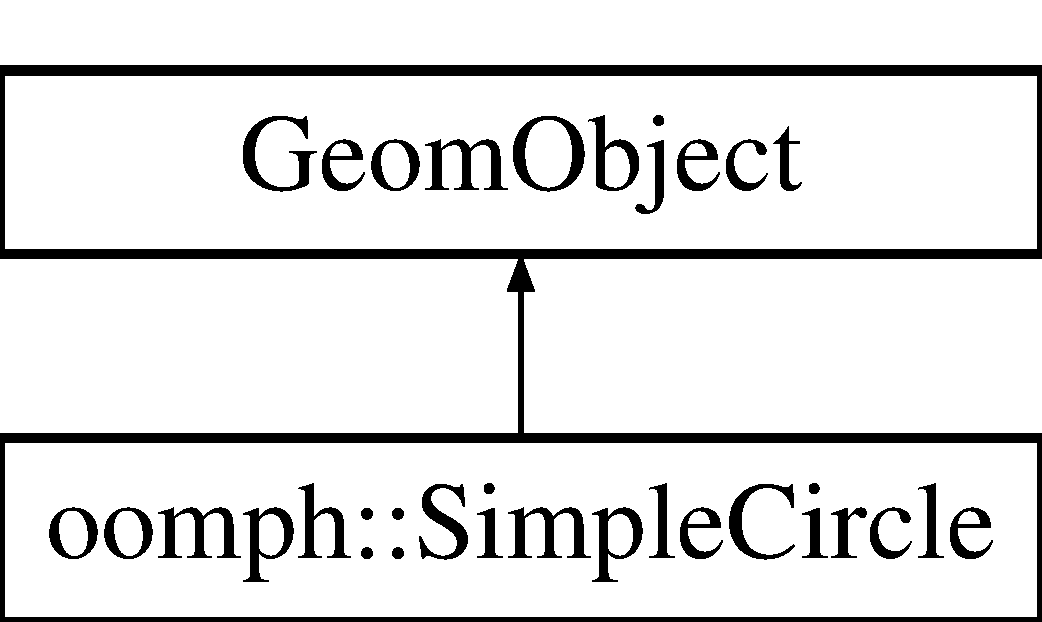
\includegraphics[height=2.000000cm]{classoomph_1_1SimpleCircle}
\end{center}
\end{figure}
\subsection*{Public Member Functions}
\begin{DoxyCompactItemize}
\item 
\hyperlink{classoomph_1_1SimpleCircle_a501ee89b2c05eebad1214b9cc4207176}{Simple\+Circle} (const double \&x\+\_\+c, const double \&y\+\_\+c, const double \&r)
\begin{DoxyCompactList}\small\item\em Constructor\+: Pass x and y-\/coords of centre and radius. \end{DoxyCompactList}\item 
void \hyperlink{classoomph_1_1SimpleCircle_a9b4e845b6e2318779a08c383d094dea5}{position} (const Vector$<$ double $>$ \&zeta, Vector$<$ double $>$ \&r) const
\begin{DoxyCompactList}\small\item\em Position Vector at Lagrangian coordinate zeta. \end{DoxyCompactList}\item 
void \hyperlink{classoomph_1_1SimpleCircle_a3718ee52794c766c9126323e62634db3}{position} (const unsigned \&t, const Vector$<$ double $>$ \&zeta, Vector$<$ double $>$ \&r) const
\begin{DoxyCompactList}\small\item\em Position Vector at Lagrangian coordinate zeta at time level t (t=0\+: present; t$>$0\+: previous level). Steady object, so we simply forward the call to the steady version. \end{DoxyCompactList}\end{DoxyCompactItemize}
\subsection*{Protected Attributes}
\begin{DoxyCompactItemize}
\item 
double \hyperlink{classoomph_1_1SimpleCircle_abd34367dbf586e6aa73314b350a370d1}{X\+\_\+c}
\begin{DoxyCompactList}\small\item\em X-\/coordinate of centre. \end{DoxyCompactList}\item 
double \hyperlink{classoomph_1_1SimpleCircle_a3f72f452d54ff683b72a15178dd5daae}{Y\+\_\+c}
\begin{DoxyCompactList}\small\item\em Y-\/coordinate of centre. \end{DoxyCompactList}\item 
double \hyperlink{classoomph_1_1SimpleCircle_afd2a653946537f867c0aaa12768f9514}{R}
\begin{DoxyCompactList}\small\item\em Radius. \end{DoxyCompactList}\end{DoxyCompactItemize}


\subsection{Detailed Description}
Simple circle in 2D space. \[ x = X_c + R \cos(\zeta) \] \[ y = Y_c + R \sin(\zeta) \]. 

Definition at line 45 of file circle.\+h.



\subsection{Constructor \& Destructor Documentation}
\mbox{\Hypertarget{classoomph_1_1SimpleCircle_a501ee89b2c05eebad1214b9cc4207176}\label{classoomph_1_1SimpleCircle_a501ee89b2c05eebad1214b9cc4207176}} 
\index{oomph\+::\+Simple\+Circle@{oomph\+::\+Simple\+Circle}!Simple\+Circle@{Simple\+Circle}}
\index{Simple\+Circle@{Simple\+Circle}!oomph\+::\+Simple\+Circle@{oomph\+::\+Simple\+Circle}}
\subsubsection{\texorpdfstring{Simple\+Circle()}{SimpleCircle()}}
{\footnotesize\ttfamily oomph\+::\+Simple\+Circle\+::\+Simple\+Circle (\begin{DoxyParamCaption}\item[{const double \&}]{x\+\_\+c,  }\item[{const double \&}]{y\+\_\+c,  }\item[{const double \&}]{r }\end{DoxyParamCaption})\hspace{0.3cm}{\ttfamily [inline]}}



Constructor\+: Pass x and y-\/coords of centre and radius. 



Definition at line 51 of file circle.\+h.



\subsection{Member Function Documentation}
\mbox{\Hypertarget{classoomph_1_1SimpleCircle_a9b4e845b6e2318779a08c383d094dea5}\label{classoomph_1_1SimpleCircle_a9b4e845b6e2318779a08c383d094dea5}} 
\index{oomph\+::\+Simple\+Circle@{oomph\+::\+Simple\+Circle}!position@{position}}
\index{position@{position}!oomph\+::\+Simple\+Circle@{oomph\+::\+Simple\+Circle}}
\subsubsection{\texorpdfstring{position()}{position()}\hspace{0.1cm}{\footnotesize\ttfamily [1/2]}}
{\footnotesize\ttfamily void oomph\+::\+Simple\+Circle\+::position (\begin{DoxyParamCaption}\item[{const Vector$<$ double $>$ \&}]{zeta,  }\item[{Vector$<$ double $>$ \&}]{r }\end{DoxyParamCaption}) const\hspace{0.3cm}{\ttfamily [inline]}}



Position Vector at Lagrangian coordinate zeta. 



Definition at line 56 of file circle.\+h.



References R, X\+\_\+c, and Y\+\_\+c.



Referenced by position(), and oomph\+::\+General\+Circle\+::position().

\mbox{\Hypertarget{classoomph_1_1SimpleCircle_a3718ee52794c766c9126323e62634db3}\label{classoomph_1_1SimpleCircle_a3718ee52794c766c9126323e62634db3}} 
\index{oomph\+::\+Simple\+Circle@{oomph\+::\+Simple\+Circle}!position@{position}}
\index{position@{position}!oomph\+::\+Simple\+Circle@{oomph\+::\+Simple\+Circle}}
\subsubsection{\texorpdfstring{position()}{position()}\hspace{0.1cm}{\footnotesize\ttfamily [2/2]}}
{\footnotesize\ttfamily void oomph\+::\+Simple\+Circle\+::position (\begin{DoxyParamCaption}\item[{const unsigned \&}]{t,  }\item[{const Vector$<$ double $>$ \&}]{zeta,  }\item[{Vector$<$ double $>$ \&}]{r }\end{DoxyParamCaption}) const\hspace{0.3cm}{\ttfamily [inline]}}



Position Vector at Lagrangian coordinate zeta at time level t (t=0\+: present; t$>$0\+: previous level). Steady object, so we simply forward the call to the steady version. 



Definition at line 66 of file circle.\+h.



References position().



\subsection{Member Data Documentation}
\mbox{\Hypertarget{classoomph_1_1SimpleCircle_afd2a653946537f867c0aaa12768f9514}\label{classoomph_1_1SimpleCircle_afd2a653946537f867c0aaa12768f9514}} 
\index{oomph\+::\+Simple\+Circle@{oomph\+::\+Simple\+Circle}!R@{R}}
\index{R@{R}!oomph\+::\+Simple\+Circle@{oomph\+::\+Simple\+Circle}}
\subsubsection{\texorpdfstring{R}{R}}
{\footnotesize\ttfamily double oomph\+::\+Simple\+Circle\+::R\hspace{0.3cm}{\ttfamily [protected]}}



Radius. 



Definition at line 79 of file circle.\+h.



Referenced by position(), and oomph\+::\+General\+Circle\+::position().

\mbox{\Hypertarget{classoomph_1_1SimpleCircle_abd34367dbf586e6aa73314b350a370d1}\label{classoomph_1_1SimpleCircle_abd34367dbf586e6aa73314b350a370d1}} 
\index{oomph\+::\+Simple\+Circle@{oomph\+::\+Simple\+Circle}!X\+\_\+c@{X\+\_\+c}}
\index{X\+\_\+c@{X\+\_\+c}!oomph\+::\+Simple\+Circle@{oomph\+::\+Simple\+Circle}}
\subsubsection{\texorpdfstring{X\+\_\+c}{X\_c}}
{\footnotesize\ttfamily double oomph\+::\+Simple\+Circle\+::\+X\+\_\+c\hspace{0.3cm}{\ttfamily [protected]}}



X-\/coordinate of centre. 



Definition at line 73 of file circle.\+h.



Referenced by position(), and oomph\+::\+General\+Circle\+::position().

\mbox{\Hypertarget{classoomph_1_1SimpleCircle_a3f72f452d54ff683b72a15178dd5daae}\label{classoomph_1_1SimpleCircle_a3f72f452d54ff683b72a15178dd5daae}} 
\index{oomph\+::\+Simple\+Circle@{oomph\+::\+Simple\+Circle}!Y\+\_\+c@{Y\+\_\+c}}
\index{Y\+\_\+c@{Y\+\_\+c}!oomph\+::\+Simple\+Circle@{oomph\+::\+Simple\+Circle}}
\subsubsection{\texorpdfstring{Y\+\_\+c}{Y\_c}}
{\footnotesize\ttfamily double oomph\+::\+Simple\+Circle\+::\+Y\+\_\+c\hspace{0.3cm}{\ttfamily [protected]}}



Y-\/coordinate of centre. 



Definition at line 76 of file circle.\+h.



Referenced by position(), and oomph\+::\+General\+Circle\+::position().



The documentation for this class was generated from the following file\+:\begin{DoxyCompactItemize}
\item 
\hyperlink{circle_8h}{circle.\+h}\end{DoxyCompactItemize}

\chapter{File Documentation}
\hypertarget{algebraic__free__boundary__poisson_8cc}{}\section{algebraic\+\_\+free\+\_\+boundary\+\_\+poisson.\+cc File Reference}
\label{algebraic__free__boundary__poisson_8cc}\index{algebraic\+\_\+free\+\_\+boundary\+\_\+poisson.\+cc@{algebraic\+\_\+free\+\_\+boundary\+\_\+poisson.\+cc}}
\subsection*{Classes}
\begin{DoxyCompactItemize}
\item 
class \hyperlink{classRefineableFishPoissonProblem}{Refineable\+Fish\+Poisson\+Problem$<$ E\+L\+E\+M\+E\+N\+T $>$}
\end{DoxyCompactItemize}
\subsection*{Namespaces}
\begin{DoxyCompactItemize}
\item 
 \hyperlink{namespaceConstSourceForPoisson}{Const\+Source\+For\+Poisson}
\begin{DoxyCompactList}\small\item\em Namespace for const source term in Poisson equation. \end{DoxyCompactList}\end{DoxyCompactItemize}
\subsection*{Functions}
\begin{DoxyCompactItemize}
\item 
void \hyperlink{namespaceConstSourceForPoisson_a40ef79083874b58ed42b4df2ca0f4c10}{Const\+Source\+For\+Poisson\+::get\+\_\+source} (const Vector$<$ double $>$ \&x, double \&source)
\begin{DoxyCompactList}\small\item\em Const source function. \end{DoxyCompactList}\item 
{\footnotesize template$<$class E\+L\+E\+M\+E\+NT $>$ }\\void \hyperlink{algebraic__free__boundary__poisson_8cc_abb923e967929c29b3a4fa1693604952a}{demo\+\_\+fish\+\_\+poisson} (const string \&directory\+\_\+name)
\item 
{\footnotesize template$<$class E\+L\+E\+M\+E\+NT $>$ }\\void \hyperlink{algebraic__free__boundary__poisson_8cc_a28565f965d7ffb7f92f3773a6333023b}{demo\+\_\+elastic\+\_\+fish\+\_\+poisson} (const string \&directory\+\_\+name)
\item 
int \hyperlink{algebraic__free__boundary__poisson_8cc_a0ddf1224851353fc92bfbff6f499fa97}{main} (int argc, char $\ast$argv\mbox{[}$\,$\mbox{]})
\end{DoxyCompactItemize}
\subsection*{Variables}
\begin{DoxyCompactItemize}
\item 
double \hyperlink{namespaceConstSourceForPoisson_add351c5acab2561d68d1fc9ec3d5fc5e}{Const\+Source\+For\+Poisson\+::\+Strength} =1.\+0
\begin{DoxyCompactList}\small\item\em Strength of source function\+: default value 1.\+0. \end{DoxyCompactList}\end{DoxyCompactItemize}


\subsection{Function Documentation}
\mbox{\Hypertarget{algebraic__free__boundary__poisson_8cc_a28565f965d7ffb7f92f3773a6333023b}\label{algebraic__free__boundary__poisson_8cc_a28565f965d7ffb7f92f3773a6333023b}} 
\index{algebraic\+\_\+free\+\_\+boundary\+\_\+poisson.\+cc@{algebraic\+\_\+free\+\_\+boundary\+\_\+poisson.\+cc}!demo\+\_\+elastic\+\_\+fish\+\_\+poisson@{demo\+\_\+elastic\+\_\+fish\+\_\+poisson}}
\index{demo\+\_\+elastic\+\_\+fish\+\_\+poisson@{demo\+\_\+elastic\+\_\+fish\+\_\+poisson}!algebraic\+\_\+free\+\_\+boundary\+\_\+poisson.\+cc@{algebraic\+\_\+free\+\_\+boundary\+\_\+poisson.\+cc}}
\subsubsection{\texorpdfstring{demo\+\_\+elastic\+\_\+fish\+\_\+poisson()}{demo\_elastic\_fish\_poisson()}}
{\footnotesize\ttfamily template$<$class E\+L\+E\+M\+E\+NT $>$ \\
void demo\+\_\+elastic\+\_\+fish\+\_\+poisson (\begin{DoxyParamCaption}\item[{const string \&}]{directory\+\_\+name }\end{DoxyParamCaption})}

Demonstrate how to solve \char`\"{}elastic\char`\"{} 2D Poisson problem in deformable fish-\/shaped domain with mesh adaptation. 

Definition at line 515 of file algebraic\+\_\+free\+\_\+boundary\+\_\+poisson.\+cc.



References Refineable\+Fish\+Poisson\+Problem$<$ E\+L\+E\+M\+E\+N\+T $>$\+::doc\+\_\+solution(), Refineable\+Fish\+Poisson\+Problem$<$ E\+L\+E\+M\+E\+N\+T $>$\+::fish\+\_\+mesh\+\_\+pt(), and Refineable\+Fish\+Poisson\+Problem$<$ E\+L\+E\+M\+E\+N\+T $>$\+::load().

\mbox{\Hypertarget{algebraic__free__boundary__poisson_8cc_abb923e967929c29b3a4fa1693604952a}\label{algebraic__free__boundary__poisson_8cc_abb923e967929c29b3a4fa1693604952a}} 
\index{algebraic\+\_\+free\+\_\+boundary\+\_\+poisson.\+cc@{algebraic\+\_\+free\+\_\+boundary\+\_\+poisson.\+cc}!demo\+\_\+fish\+\_\+poisson@{demo\+\_\+fish\+\_\+poisson}}
\index{demo\+\_\+fish\+\_\+poisson@{demo\+\_\+fish\+\_\+poisson}!algebraic\+\_\+free\+\_\+boundary\+\_\+poisson.\+cc@{algebraic\+\_\+free\+\_\+boundary\+\_\+poisson.\+cc}}
\subsubsection{\texorpdfstring{demo\+\_\+fish\+\_\+poisson()}{demo\_fish\_poisson()}}
{\footnotesize\ttfamily template$<$class E\+L\+E\+M\+E\+NT $>$ \\
void demo\+\_\+fish\+\_\+poisson (\begin{DoxyParamCaption}\item[{const string \&}]{directory\+\_\+name }\end{DoxyParamCaption})}

Demonstrate how to solve 2D Poisson problem in deformable fish-\/shaped domain with mesh adaptation. 

Definition at line 464 of file algebraic\+\_\+free\+\_\+boundary\+\_\+poisson.\+cc.



References Refineable\+Fish\+Poisson\+Problem$<$ E\+L\+E\+M\+E\+N\+T $>$\+::doc\+\_\+info(), Refineable\+Fish\+Poisson\+Problem$<$ E\+L\+E\+M\+E\+N\+T $>$\+::doc\+\_\+solution(), Refineable\+Fish\+Poisson\+Problem$<$ E\+L\+E\+M\+E\+N\+T $>$\+::fish\+\_\+mesh\+\_\+pt(), and Refineable\+Fish\+Poisson\+Problem$<$ E\+L\+E\+M\+E\+N\+T $>$\+::y\+\_\+c().

\mbox{\Hypertarget{algebraic__free__boundary__poisson_8cc_a0ddf1224851353fc92bfbff6f499fa97}\label{algebraic__free__boundary__poisson_8cc_a0ddf1224851353fc92bfbff6f499fa97}} 
\index{algebraic\+\_\+free\+\_\+boundary\+\_\+poisson.\+cc@{algebraic\+\_\+free\+\_\+boundary\+\_\+poisson.\+cc}!main@{main}}
\index{main@{main}!algebraic\+\_\+free\+\_\+boundary\+\_\+poisson.\+cc@{algebraic\+\_\+free\+\_\+boundary\+\_\+poisson.\+cc}}
\subsubsection{\texorpdfstring{main()}{main()}}
{\footnotesize\ttfamily int main (\begin{DoxyParamCaption}\item[{int}]{argc,  }\item[{char $\ast$}]{argv\mbox{[}$\,$\mbox{]} }\end{DoxyParamCaption})}

Driver for \char`\"{}elastic\char`\"{} fish poisson solver with adaptation. If there are any command line arguments, we regard this as a validation run and perform only a single step. 

Definition at line 562 of file algebraic\+\_\+free\+\_\+boundary\+\_\+poisson.\+cc.


\hypertarget{circle_8cc}{}\section{circle.\+cc File Reference}
\label{circle_8cc}\index{circle.\+cc@{circle.\+cc}}
\subsection*{Functions}
\begin{DoxyCompactItemize}
\item 
int \hyperlink{circle_8cc_ae66f6b31b5ad750f1fe042a706a4e3d4}{main} ()
\begin{DoxyCompactList}\small\item\em Driver. \end{DoxyCompactList}\end{DoxyCompactItemize}


\subsection{Function Documentation}
\mbox{\Hypertarget{circle_8cc_ae66f6b31b5ad750f1fe042a706a4e3d4}\label{circle_8cc_ae66f6b31b5ad750f1fe042a706a4e3d4}} 
\index{circle.\+cc@{circle.\+cc}!main@{main}}
\index{main@{main}!circle.\+cc@{circle.\+cc}}
\subsubsection{\texorpdfstring{main()}{main()}}
{\footnotesize\ttfamily int main (\begin{DoxyParamCaption}{ }\end{DoxyParamCaption})}



Driver. 



Definition at line 44 of file circle.\+cc.



References oomph\+::\+General\+Circle\+::position().


\hypertarget{circle_8h}{}\section{circle.\+h File Reference}
\label{circle_8h}\index{circle.\+h@{circle.\+h}}
\subsection*{Classes}
\begin{DoxyCompactItemize}
\item 
class \hyperlink{classoomph_1_1SimpleCircle}{oomph\+::\+Simple\+Circle}
\begin{DoxyCompactList}\small\item\em Simple circle in 2D space. \[ x = X_c + R \cos(\zeta) \] \[ y = Y_c + R \sin(\zeta) \]. \end{DoxyCompactList}\item 
class \hyperlink{classoomph_1_1GeneralCircle}{oomph\+::\+General\+Circle}
\begin{DoxyCompactList}\small\item\em \hyperlink{classoomph_1_1GeneralCircle}{General\+Circle} in 2D space. \[ x = X_c + R \cos(\zeta) \] \[ y = Y_c + R \sin(\zeta) \] The three parameters $ X_c, Y_c $ and $ R $ are represented by Data and can therefore be unknowns in the problem. \end{DoxyCompactList}\end{DoxyCompactItemize}
\subsection*{Namespaces}
\begin{DoxyCompactItemize}
\item 
 \hyperlink{namespaceoomph}{oomph}
\end{DoxyCompactItemize}

\hypertarget{circle__as__generalised__element_8h}{}\section{circle\+\_\+as\+\_\+generalised\+\_\+element.\+h File Reference}
\label{circle__as__generalised__element_8h}\index{circle\+\_\+as\+\_\+generalised\+\_\+element.\+h@{circle\+\_\+as\+\_\+generalised\+\_\+element.\+h}}
\subsection*{Classes}
\begin{DoxyCompactItemize}
\item 
class \hyperlink{classoomph_1_1ElasticallySupportedRingElement}{oomph\+::\+Elastically\+Supported\+Ring\+Element}
\begin{DoxyCompactList}\small\item\em \hyperlink{classoomph_1_1GeneralCircle}{General\+Circle} \char`\"{}upgraded\char`\"{} to a Generalised\+Element\+: Circular ring whose position is given by \[ x = X_c + R \cos(\zeta) \] \[ y = Y_c + R \sin(\zeta) \] The ring\textquotesingle{}s vertical position $ Y_c $ is determined by \char`\"{}pseudo elasticity\char`\"{}\+: \[ 0 = f_{load} - Y_c \ k_{stiff} \] This simulates the case where the centre of the ring is mounted on an elastic spring of stiffness $ k_{stiff} $ and loaded by the force $ f_{load}. $ The \char`\"{}load\char`\"{} is specified by the Data object {\ttfamily load\+\_\+pt()}. \end{DoxyCompactList}\end{DoxyCompactItemize}
\subsection*{Namespaces}
\begin{DoxyCompactItemize}
\item 
 \hyperlink{namespaceoomph}{oomph}
\end{DoxyCompactItemize}

\hypertarget{doc__sparse__macro__node__update_8cc}{}\section{doc\+\_\+sparse\+\_\+macro\+\_\+node\+\_\+update.\+cc File Reference}
\label{doc__sparse__macro__node__update_8cc}\index{doc\+\_\+sparse\+\_\+macro\+\_\+node\+\_\+update.\+cc@{doc\+\_\+sparse\+\_\+macro\+\_\+node\+\_\+update.\+cc}}
\subsection*{Functions}
\begin{DoxyCompactItemize}
\item 
int \hyperlink{doc__sparse__macro__node__update_8cc_ae66f6b31b5ad750f1fe042a706a4e3d4}{main} ()
\begin{DoxyCompactList}\small\item\em Driver to document sparse Macro\+Element-\/based node update. \end{DoxyCompactList}\end{DoxyCompactItemize}


\subsection{Function Documentation}
\mbox{\Hypertarget{doc__sparse__macro__node__update_8cc_ae66f6b31b5ad750f1fe042a706a4e3d4}\label{doc__sparse__macro__node__update_8cc_ae66f6b31b5ad750f1fe042a706a4e3d4}} 
\index{doc\+\_\+sparse\+\_\+macro\+\_\+node\+\_\+update.\+cc@{doc\+\_\+sparse\+\_\+macro\+\_\+node\+\_\+update.\+cc}!main@{main}}
\index{main@{main}!doc\+\_\+sparse\+\_\+macro\+\_\+node\+\_\+update.\+cc@{doc\+\_\+sparse\+\_\+macro\+\_\+node\+\_\+update.\+cc}}
\subsubsection{\texorpdfstring{main()}{main()}}
{\footnotesize\ttfamily int main (\begin{DoxyParamCaption}{ }\end{DoxyParamCaption})}



Driver to document sparse Macro\+Element-\/based node update. 



Definition at line 52 of file doc\+\_\+sparse\+\_\+macro\+\_\+node\+\_\+update.\+cc.



References oomph\+::\+General\+Circle\+::y\+\_\+c().


\hypertarget{elastic__mesh__update_8cc}{}\section{elastic\+\_\+mesh\+\_\+update.\+cc File Reference}
\label{elastic__mesh__update_8cc}\index{elastic\+\_\+mesh\+\_\+update.\+cc@{elastic\+\_\+mesh\+\_\+update.\+cc}}
\subsection*{Classes}
\begin{DoxyCompactItemize}
\item 
class \hyperlink{classElasticFishMesh}{Elastic\+Fish\+Mesh$<$ E\+L\+E\+M\+E\+N\+T $>$}
\begin{DoxyCompactList}\small\item\em Refineable fish mesh upgraded to become a solid mesh. \end{DoxyCompactList}\item 
class \hyperlink{classDeformableFishPoissonProblem}{Deformable\+Fish\+Poisson\+Problem$<$ E\+L\+E\+M\+E\+N\+T $>$}
\end{DoxyCompactItemize}
\subsection*{Namespaces}
\begin{DoxyCompactItemize}
\item 
 \hyperlink{namespaceConstSourceForPoisson}{Const\+Source\+For\+Poisson}
\begin{DoxyCompactList}\small\item\em Namespace for const source term in Poisson equation. \end{DoxyCompactList}\item 
 \hyperlink{namespaceGlobal__Physical__Variables}{Global\+\_\+\+Physical\+\_\+\+Variables}
\begin{DoxyCompactList}\small\item\em Global variables. \end{DoxyCompactList}\end{DoxyCompactItemize}
\subsection*{Functions}
\begin{DoxyCompactItemize}
\item 
void \hyperlink{namespaceConstSourceForPoisson_a40ef79083874b58ed42b4df2ca0f4c10}{Const\+Source\+For\+Poisson\+::get\+\_\+source} (const Vector$<$ double $>$ \&x, double \&source)
\begin{DoxyCompactList}\small\item\em Const source function. \end{DoxyCompactList}\item 
int \hyperlink{elastic__mesh__update_8cc_a0ddf1224851353fc92bfbff6f499fa97}{main} (int argc, char $\ast$argv\mbox{[}$\,$\mbox{]})
\end{DoxyCompactItemize}
\subsection*{Variables}
\begin{DoxyCompactItemize}
\item 
Constitutive\+Law $\ast$ \hyperlink{namespaceGlobal__Physical__Variables_a5d5f19442938130d36ee7476ae25049c}{Global\+\_\+\+Physical\+\_\+\+Variables\+::\+Constitutive\+\_\+law\+\_\+pt}
\begin{DoxyCompactList}\small\item\em Pointer to constitutive law. \end{DoxyCompactList}\item 
double \hyperlink{namespaceGlobal__Physical__Variables_a3962c36313826b19f216f6bbbdd6a477}{Global\+\_\+\+Physical\+\_\+\+Variables\+::\+Nu} =0.\+3
\begin{DoxyCompactList}\small\item\em Poisson\textquotesingle{}s ratio. \end{DoxyCompactList}\end{DoxyCompactItemize}


\subsection{Function Documentation}
\mbox{\Hypertarget{elastic__mesh__update_8cc_a0ddf1224851353fc92bfbff6f499fa97}\label{elastic__mesh__update_8cc_a0ddf1224851353fc92bfbff6f499fa97}} 
\index{elastic\+\_\+mesh\+\_\+update.\+cc@{elastic\+\_\+mesh\+\_\+update.\+cc}!main@{main}}
\index{main@{main}!elastic\+\_\+mesh\+\_\+update.\+cc@{elastic\+\_\+mesh\+\_\+update.\+cc}}
\subsubsection{\texorpdfstring{main()}{main()}}
{\footnotesize\ttfamily int main (\begin{DoxyParamCaption}\item[{int}]{argc,  }\item[{char $\ast$}]{argv\mbox{[}$\,$\mbox{]} }\end{DoxyParamCaption})}

Driver for simple elastic problem. If there are any command line arguments, we regard this as a validation run and perform only a single step. 

Definition at line 464 of file elastic\+\_\+mesh\+\_\+update.\+cc.



References Global\+\_\+\+Physical\+\_\+\+Variables\+::\+Constitutive\+\_\+law\+\_\+pt, Global\+\_\+\+Physical\+\_\+\+Variables\+::\+Nu, and Deformable\+Fish\+Poisson\+Problem$<$ E\+L\+E\+M\+E\+N\+T $>$\+::run().


\hypertarget{elastic__poisson_8cc}{}\section{elastic\+\_\+poisson.\+cc File Reference}
\label{elastic__poisson_8cc}\index{elastic\+\_\+poisson.\+cc@{elastic\+\_\+poisson.\+cc}}
\subsection*{Classes}
\begin{DoxyCompactItemize}
\item 
class \hyperlink{classElasticFishBackElement}{Elastic\+Fish\+Back\+Element}
\begin{DoxyCompactList}\small\item\em Fish back as a Generalised\+Element\+: Circular ring whose position is given by \[ x = X_c + R \cos(\xi) \] \[ y = Y_c + R \sin(\xi) \] The ring\textquotesingle{}s vertical position $ Y_c $ is determined by \char`\"{}pseudo elasticity\char`\"{}\+: \[ 0 = Y_c \ k_{stiff} - f_{load} \] This simulates the case where the centre of the ring is mounted on an elastic spring of stiffness $ k_{stiff} $ and loaded by the force $ f_{load}. $ The \char`\"{}load\char`\"{} is specified by the Data object {\ttfamily load\+\_\+pt()}. \end{DoxyCompactList}\item 
class \hyperlink{classRefineableFishPoissonProblem}{Refineable\+Fish\+Poisson\+Problem$<$ E\+L\+E\+M\+E\+N\+T $>$}
\end{DoxyCompactItemize}
\subsection*{Namespaces}
\begin{DoxyCompactItemize}
\item 
 \hyperlink{namespaceConstSourceForPoisson}{Const\+Source\+For\+Poisson}
\begin{DoxyCompactList}\small\item\em Namespace for const source term in Poisson equation. \end{DoxyCompactList}\end{DoxyCompactItemize}
\subsection*{Functions}
\begin{DoxyCompactItemize}
\item 
void \hyperlink{namespaceConstSourceForPoisson_a40ef79083874b58ed42b4df2ca0f4c10}{Const\+Source\+For\+Poisson\+::get\+\_\+source} (const Vector$<$ double $>$ \&x, double \&source)
\begin{DoxyCompactList}\small\item\em Const source function. \end{DoxyCompactList}\item 
{\footnotesize template$<$class E\+L\+E\+M\+E\+NT $>$ }\\void \hyperlink{elastic__poisson_8cc_abb923e967929c29b3a4fa1693604952a}{demo\+\_\+fish\+\_\+poisson} (const string \&directory\+\_\+name)
\item 
{\footnotesize template$<$class E\+L\+E\+M\+E\+NT $>$ }\\void \hyperlink{elastic__poisson_8cc_a28565f965d7ffb7f92f3773a6333023b}{demo\+\_\+elastic\+\_\+fish\+\_\+poisson} (const string \&directory\+\_\+name)
\item 
int \hyperlink{elastic__poisson_8cc_a0ddf1224851353fc92bfbff6f499fa97}{main} (int argc, char $\ast$argv\mbox{[}$\,$\mbox{]})
\end{DoxyCompactItemize}
\subsection*{Variables}
\begin{DoxyCompactItemize}
\item 
double \hyperlink{namespaceConstSourceForPoisson_add351c5acab2561d68d1fc9ec3d5fc5e}{Const\+Source\+For\+Poisson\+::\+Strength} =1.\+0
\begin{DoxyCompactList}\small\item\em Strength of source function\+: default value 1.\+0. \end{DoxyCompactList}\end{DoxyCompactItemize}


\subsection{Function Documentation}
\mbox{\Hypertarget{elastic__poisson_8cc_a28565f965d7ffb7f92f3773a6333023b}\label{elastic__poisson_8cc_a28565f965d7ffb7f92f3773a6333023b}} 
\index{elastic\+\_\+poisson.\+cc@{elastic\+\_\+poisson.\+cc}!demo\+\_\+elastic\+\_\+fish\+\_\+poisson@{demo\+\_\+elastic\+\_\+fish\+\_\+poisson}}
\index{demo\+\_\+elastic\+\_\+fish\+\_\+poisson@{demo\+\_\+elastic\+\_\+fish\+\_\+poisson}!elastic\+\_\+poisson.\+cc@{elastic\+\_\+poisson.\+cc}}
\subsubsection{\texorpdfstring{demo\+\_\+elastic\+\_\+fish\+\_\+poisson()}{demo\_elastic\_fish\_poisson()}}
{\footnotesize\ttfamily template$<$class E\+L\+E\+M\+E\+NT $>$ \\
void demo\+\_\+elastic\+\_\+fish\+\_\+poisson (\begin{DoxyParamCaption}\item[{const string \&}]{directory\+\_\+name }\end{DoxyParamCaption})}

Demonstrate how to solve \char`\"{}elastic\char`\"{} 2D Poisson problem in deformable fish-\/shaped domain with mesh adaptation. 

Definition at line 582 of file elastic\+\_\+poisson.\+cc.



References Refineable\+Fish\+Poisson\+Problem$<$ E\+L\+E\+M\+E\+N\+T $>$\+::doc\+\_\+solution(), Refineable\+Fish\+Poisson\+Problem$<$ E\+L\+E\+M\+E\+N\+T $>$\+::fish\+\_\+mesh\+\_\+pt(), and Refineable\+Fish\+Poisson\+Problem$<$ E\+L\+E\+M\+E\+N\+T $>$\+::load().

\mbox{\Hypertarget{elastic__poisson_8cc_abb923e967929c29b3a4fa1693604952a}\label{elastic__poisson_8cc_abb923e967929c29b3a4fa1693604952a}} 
\index{elastic\+\_\+poisson.\+cc@{elastic\+\_\+poisson.\+cc}!demo\+\_\+fish\+\_\+poisson@{demo\+\_\+fish\+\_\+poisson}}
\index{demo\+\_\+fish\+\_\+poisson@{demo\+\_\+fish\+\_\+poisson}!elastic\+\_\+poisson.\+cc@{elastic\+\_\+poisson.\+cc}}
\subsubsection{\texorpdfstring{demo\+\_\+fish\+\_\+poisson()}{demo\_fish\_poisson()}}
{\footnotesize\ttfamily template$<$class E\+L\+E\+M\+E\+NT $>$ \\
void demo\+\_\+fish\+\_\+poisson (\begin{DoxyParamCaption}\item[{const string \&}]{directory\+\_\+name }\end{DoxyParamCaption})}

Demonstrate how to solve 2D Poisson problem in deformable fish-\/shaped domain with mesh adaptation. 

Definition at line 533 of file elastic\+\_\+poisson.\+cc.



References Refineable\+Fish\+Poisson\+Problem$<$ E\+L\+E\+M\+E\+N\+T $>$\+::doc\+\_\+info(), Refineable\+Fish\+Poisson\+Problem$<$ E\+L\+E\+M\+E\+N\+T $>$\+::doc\+\_\+solution(), Refineable\+Fish\+Poisson\+Problem$<$ E\+L\+E\+M\+E\+N\+T $>$\+::fish\+\_\+mesh\+\_\+pt(), and Refineable\+Fish\+Poisson\+Problem$<$ E\+L\+E\+M\+E\+N\+T $>$\+::load().

\mbox{\Hypertarget{elastic__poisson_8cc_a0ddf1224851353fc92bfbff6f499fa97}\label{elastic__poisson_8cc_a0ddf1224851353fc92bfbff6f499fa97}} 
\index{elastic\+\_\+poisson.\+cc@{elastic\+\_\+poisson.\+cc}!main@{main}}
\index{main@{main}!elastic\+\_\+poisson.\+cc@{elastic\+\_\+poisson.\+cc}}
\subsubsection{\texorpdfstring{main()}{main()}}
{\footnotesize\ttfamily int main (\begin{DoxyParamCaption}\item[{int}]{argc,  }\item[{char $\ast$}]{argv\mbox{[}$\,$\mbox{]} }\end{DoxyParamCaption})}

Driver for \char`\"{}elastic\char`\"{} fish poisson solver with adaptation. If there are any command line arguments, we regard this as a validation run and perform only a single step. 

Definition at line 617 of file elastic\+\_\+poisson.\+cc.


\hypertarget{elastic__poisson_8txt__doxygenified_8h}{}\section{elastic\+\_\+poisson.\+txt\+\_\+doxygenified.\+h File Reference}
\label{elastic__poisson_8txt__doxygenified_8h}\index{elastic\+\_\+poisson.\+txt\+\_\+doxygenified.\+h@{elastic\+\_\+poisson.\+txt\+\_\+doxygenified.\+h}}

\hypertarget{geom__object__element_8cc}{}\section{geom\+\_\+object\+\_\+element.\+cc File Reference}
\label{geom__object__element_8cc}\index{geom\+\_\+object\+\_\+element.\+cc@{geom\+\_\+object\+\_\+element.\+cc}}
\subsection*{Classes}
\begin{DoxyCompactItemize}
\item 
class \hyperlink{classGeomObjectAsGeneralisedElementProblem}{Geom\+Object\+As\+Generalised\+Element\+Problem}
\end{DoxyCompactItemize}
\subsection*{Functions}
\begin{DoxyCompactItemize}
\item 
int \hyperlink{geom__object__element_8cc_ae66f6b31b5ad750f1fe042a706a4e3d4}{main} ()
\begin{DoxyCompactList}\small\item\em Driver. \end{DoxyCompactList}\end{DoxyCompactItemize}


\subsection{Function Documentation}
\mbox{\Hypertarget{geom__object__element_8cc_ae66f6b31b5ad750f1fe042a706a4e3d4}\label{geom__object__element_8cc_ae66f6b31b5ad750f1fe042a706a4e3d4}} 
\index{geom\+\_\+object\+\_\+element.\+cc@{geom\+\_\+object\+\_\+element.\+cc}!main@{main}}
\index{main@{main}!geom\+\_\+object\+\_\+element.\+cc@{geom\+\_\+object\+\_\+element.\+cc}}
\subsubsection{\texorpdfstring{main()}{main()}}
{\footnotesize\ttfamily int main (\begin{DoxyParamCaption}{ }\end{DoxyParamCaption})}



Driver. 



Definition at line 212 of file geom\+\_\+object\+\_\+element.\+cc.



References Geom\+Object\+As\+Generalised\+Element\+Problem\+::doc\+\_\+info(), Geom\+Object\+As\+Generalised\+Element\+Problem\+::doc\+\_\+solution(), and Geom\+Object\+As\+Generalised\+Element\+Problem\+::load().


\hypertarget{macro__element__free__boundary__poisson_8cc}{}\section{macro\+\_\+element\+\_\+free\+\_\+boundary\+\_\+poisson.\+cc File Reference}
\label{macro__element__free__boundary__poisson_8cc}\index{macro\+\_\+element\+\_\+free\+\_\+boundary\+\_\+poisson.\+cc@{macro\+\_\+element\+\_\+free\+\_\+boundary\+\_\+poisson.\+cc}}
\subsection*{Classes}
\begin{DoxyCompactItemize}
\item 
class \hyperlink{classMyMacroElementNodeUpdateRefineableFishMesh}{My\+Macro\+Element\+Node\+Update\+Refineable\+Fish\+Mesh$<$ E\+L\+E\+M\+E\+N\+T $>$}
\begin{DoxyCompactList}\small\item\em Refineable, fish-\/shaped mesh with Macro\+Element-\/based node update. \end{DoxyCompactList}\item 
class \hyperlink{classFreeBoundaryPoissonProblem}{Free\+Boundary\+Poisson\+Problem$<$ E\+L\+E\+M\+E\+N\+T $>$}
\end{DoxyCompactItemize}
\subsection*{Namespaces}
\begin{DoxyCompactItemize}
\item 
 \hyperlink{namespaceConstSourceForPoisson}{Const\+Source\+For\+Poisson}
\begin{DoxyCompactList}\small\item\em Namespace for const source term in Poisson equation. \end{DoxyCompactList}\end{DoxyCompactItemize}
\subsection*{Functions}
\begin{DoxyCompactItemize}
\item 
void \hyperlink{namespaceConstSourceForPoisson_a40ef79083874b58ed42b4df2ca0f4c10}{Const\+Source\+For\+Poisson\+::get\+\_\+source} (const Vector$<$ double $>$ \&x, double \&source)
\begin{DoxyCompactList}\small\item\em Const source function. \end{DoxyCompactList}\item 
int \hyperlink{macro__element__free__boundary__poisson_8cc_ae66f6b31b5ad750f1fe042a706a4e3d4}{main} ()
\begin{DoxyCompactList}\small\item\em Driver for \char`\"{}free-\/boundary\char`\"{} fish poisson solver with adaptation. \end{DoxyCompactList}\end{DoxyCompactItemize}


\subsection{Function Documentation}
\mbox{\Hypertarget{macro__element__free__boundary__poisson_8cc_ae66f6b31b5ad750f1fe042a706a4e3d4}\label{macro__element__free__boundary__poisson_8cc_ae66f6b31b5ad750f1fe042a706a4e3d4}} 
\index{macro\+\_\+element\+\_\+free\+\_\+boundary\+\_\+poisson.\+cc@{macro\+\_\+element\+\_\+free\+\_\+boundary\+\_\+poisson.\+cc}!main@{main}}
\index{main@{main}!macro\+\_\+element\+\_\+free\+\_\+boundary\+\_\+poisson.\+cc@{macro\+\_\+element\+\_\+free\+\_\+boundary\+\_\+poisson.\+cc}}
\subsubsection{\texorpdfstring{main()}{main()}}
{\footnotesize\ttfamily int main (\begin{DoxyParamCaption}{ }\end{DoxyParamCaption})}



Driver for \char`\"{}free-\/boundary\char`\"{} fish poisson solver with adaptation. 



Definition at line 312 of file macro\+\_\+element\+\_\+free\+\_\+boundary\+\_\+poisson.\+cc.



References Free\+Boundary\+Poisson\+Problem$<$ E\+L\+E\+M\+E\+N\+T $>$\+::doc\+\_\+solution().


\hypertarget{macro__element__free__boundary__poisson__non__ref_8cc}{}\section{macro\+\_\+element\+\_\+free\+\_\+boundary\+\_\+poisson\+\_\+non\+\_\+ref.\+cc File Reference}
\label{macro__element__free__boundary__poisson__non__ref_8cc}\index{macro\+\_\+element\+\_\+free\+\_\+boundary\+\_\+poisson\+\_\+non\+\_\+ref.\+cc@{macro\+\_\+element\+\_\+free\+\_\+boundary\+\_\+poisson\+\_\+non\+\_\+ref.\+cc}}
\subsection*{Classes}
\begin{DoxyCompactItemize}
\item 
class \hyperlink{classMyMacroElementNodeUpdateFishMesh}{My\+Macro\+Element\+Node\+Update\+Fish\+Mesh$<$ E\+L\+E\+M\+E\+N\+T $>$}
\begin{DoxyCompactList}\small\item\em Fish-\/shaped mesh with Macro\+Element-\/based node update. \end{DoxyCompactList}\item 
class \hyperlink{classFreeBoundaryPoissonProblem}{Free\+Boundary\+Poisson\+Problem$<$ E\+L\+E\+M\+E\+N\+T $>$}
\end{DoxyCompactItemize}
\subsection*{Namespaces}
\begin{DoxyCompactItemize}
\item 
 \hyperlink{namespaceConstSourceForPoisson}{Const\+Source\+For\+Poisson}
\begin{DoxyCompactList}\small\item\em Namespace for const source term in Poisson equation. \end{DoxyCompactList}\end{DoxyCompactItemize}
\subsection*{Functions}
\begin{DoxyCompactItemize}
\item 
void \hyperlink{namespaceConstSourceForPoisson_a40ef79083874b58ed42b4df2ca0f4c10}{Const\+Source\+For\+Poisson\+::get\+\_\+source} (const Vector$<$ double $>$ \&x, double \&source)
\begin{DoxyCompactList}\small\item\em Const source function. \end{DoxyCompactList}\item 
int \hyperlink{macro__element__free__boundary__poisson__non__ref_8cc_ae66f6b31b5ad750f1fe042a706a4e3d4}{main} ()
\begin{DoxyCompactList}\small\item\em Driver for \char`\"{}free-\/boundary\char`\"{} fish poisson solver with adaptation. \end{DoxyCompactList}\end{DoxyCompactItemize}


\subsection{Function Documentation}
\mbox{\Hypertarget{macro__element__free__boundary__poisson__non__ref_8cc_ae66f6b31b5ad750f1fe042a706a4e3d4}\label{macro__element__free__boundary__poisson__non__ref_8cc_ae66f6b31b5ad750f1fe042a706a4e3d4}} 
\index{macro\+\_\+element\+\_\+free\+\_\+boundary\+\_\+poisson\+\_\+non\+\_\+ref.\+cc@{macro\+\_\+element\+\_\+free\+\_\+boundary\+\_\+poisson\+\_\+non\+\_\+ref.\+cc}!main@{main}}
\index{main@{main}!macro\+\_\+element\+\_\+free\+\_\+boundary\+\_\+poisson\+\_\+non\+\_\+ref.\+cc@{macro\+\_\+element\+\_\+free\+\_\+boundary\+\_\+poisson\+\_\+non\+\_\+ref.\+cc}}
\subsubsection{\texorpdfstring{main()}{main()}}
{\footnotesize\ttfamily int main (\begin{DoxyParamCaption}{ }\end{DoxyParamCaption})}



Driver for \char`\"{}free-\/boundary\char`\"{} fish poisson solver with adaptation. 



Definition at line 310 of file macro\+\_\+element\+\_\+free\+\_\+boundary\+\_\+poisson\+\_\+non\+\_\+ref.\+cc.



References Free\+Boundary\+Poisson\+Problem$<$ E\+L\+E\+M\+E\+N\+T $>$\+::doc\+\_\+solution().


\hypertarget{old__for__doc_8cc}{}\section{old\+\_\+for\+\_\+doc.\+cc File Reference}
\label{old__for__doc_8cc}\index{old\+\_\+for\+\_\+doc.\+cc@{old\+\_\+for\+\_\+doc.\+cc}}
\subsection*{Classes}
\begin{DoxyCompactItemize}
\item 
class \hyperlink{classRefineableFishPoissonProblem}{Refineable\+Fish\+Poisson\+Problem$<$ E\+L\+E\+M\+E\+N\+T $>$}
\end{DoxyCompactItemize}
\subsection*{Namespaces}
\begin{DoxyCompactItemize}
\item 
 \hyperlink{namespaceConstSourceForPoisson}{Const\+Source\+For\+Poisson}
\begin{DoxyCompactList}\small\item\em Namespace for const source term in Poisson equation. \end{DoxyCompactList}\end{DoxyCompactItemize}
\subsection*{Functions}
\begin{DoxyCompactItemize}
\item 
void \hyperlink{namespaceConstSourceForPoisson_a40ef79083874b58ed42b4df2ca0f4c10}{Const\+Source\+For\+Poisson\+::get\+\_\+source} (const Vector$<$ double $>$ \&x, double \&source)
\begin{DoxyCompactList}\small\item\em Const source function. \end{DoxyCompactList}\item 
{\footnotesize template$<$class E\+L\+E\+M\+E\+NT $>$ }\\void \hyperlink{old__for__doc_8cc_abb923e967929c29b3a4fa1693604952a}{demo\+\_\+fish\+\_\+poisson} (const string \&directory\+\_\+name)
\item 
{\footnotesize template$<$class E\+L\+E\+M\+E\+NT $>$ }\\void \hyperlink{old__for__doc_8cc_a28565f965d7ffb7f92f3773a6333023b}{demo\+\_\+elastic\+\_\+fish\+\_\+poisson} (const string \&directory\+\_\+name)
\item 
int \hyperlink{old__for__doc_8cc_a0ddf1224851353fc92bfbff6f499fa97}{main} (int argc, char $\ast$argv\mbox{[}$\,$\mbox{]})
\end{DoxyCompactItemize}


\subsection{Function Documentation}
\mbox{\Hypertarget{old__for__doc_8cc_a28565f965d7ffb7f92f3773a6333023b}\label{old__for__doc_8cc_a28565f965d7ffb7f92f3773a6333023b}} 
\index{old\+\_\+for\+\_\+doc.\+cc@{old\+\_\+for\+\_\+doc.\+cc}!demo\+\_\+elastic\+\_\+fish\+\_\+poisson@{demo\+\_\+elastic\+\_\+fish\+\_\+poisson}}
\index{demo\+\_\+elastic\+\_\+fish\+\_\+poisson@{demo\+\_\+elastic\+\_\+fish\+\_\+poisson}!old\+\_\+for\+\_\+doc.\+cc@{old\+\_\+for\+\_\+doc.\+cc}}
\subsubsection{\texorpdfstring{demo\+\_\+elastic\+\_\+fish\+\_\+poisson()}{demo\_elastic\_fish\_poisson()}}
{\footnotesize\ttfamily template$<$class E\+L\+E\+M\+E\+NT $>$ \\
void demo\+\_\+elastic\+\_\+fish\+\_\+poisson (\begin{DoxyParamCaption}\item[{const string \&}]{directory\+\_\+name }\end{DoxyParamCaption})}

Demonstrate how to solve coupled \char`\"{}elastic\char`\"{} 2D Poisson problem in deformable fish-\/shaped domain with mesh adaptation. 

Definition at line 450 of file old\+\_\+for\+\_\+doc.\+cc.



References Refineable\+Fish\+Poisson\+Problem$<$ E\+L\+E\+M\+E\+N\+T $>$\+::doc\+\_\+solution(), Refineable\+Fish\+Poisson\+Problem$<$ E\+L\+E\+M\+E\+N\+T $>$\+::fish\+\_\+mesh\+\_\+pt(), and Refineable\+Fish\+Poisson\+Problem$<$ E\+L\+E\+M\+E\+N\+T $>$\+::load().

\mbox{\Hypertarget{old__for__doc_8cc_abb923e967929c29b3a4fa1693604952a}\label{old__for__doc_8cc_abb923e967929c29b3a4fa1693604952a}} 
\index{old\+\_\+for\+\_\+doc.\+cc@{old\+\_\+for\+\_\+doc.\+cc}!demo\+\_\+fish\+\_\+poisson@{demo\+\_\+fish\+\_\+poisson}}
\index{demo\+\_\+fish\+\_\+poisson@{demo\+\_\+fish\+\_\+poisson}!old\+\_\+for\+\_\+doc.\+cc@{old\+\_\+for\+\_\+doc.\+cc}}
\subsubsection{\texorpdfstring{demo\+\_\+fish\+\_\+poisson()}{demo\_fish\_poisson()}}
{\footnotesize\ttfamily template$<$class E\+L\+E\+M\+E\+NT $>$ \\
void demo\+\_\+fish\+\_\+poisson (\begin{DoxyParamCaption}\item[{const string \&}]{directory\+\_\+name }\end{DoxyParamCaption})}

Demonstrate how to solve 2D Poisson problem in deformable fish-\/shaped domain with mesh adaptation. 

Definition at line 387 of file old\+\_\+for\+\_\+doc.\+cc.



References Refineable\+Fish\+Poisson\+Problem$<$ E\+L\+E\+M\+E\+N\+T $>$\+::doc\+\_\+info(), Refineable\+Fish\+Poisson\+Problem$<$ E\+L\+E\+M\+E\+N\+T $>$\+::doc\+\_\+solution(), Refineable\+Fish\+Poisson\+Problem$<$ E\+L\+E\+M\+E\+N\+T $>$\+::fish\+\_\+mesh\+\_\+pt(), and Refineable\+Fish\+Poisson\+Problem$<$ E\+L\+E\+M\+E\+N\+T $>$\+::y\+\_\+c().

\mbox{\Hypertarget{old__for__doc_8cc_a0ddf1224851353fc92bfbff6f499fa97}\label{old__for__doc_8cc_a0ddf1224851353fc92bfbff6f499fa97}} 
\index{old\+\_\+for\+\_\+doc.\+cc@{old\+\_\+for\+\_\+doc.\+cc}!main@{main}}
\index{main@{main}!old\+\_\+for\+\_\+doc.\+cc@{old\+\_\+for\+\_\+doc.\+cc}}
\subsubsection{\texorpdfstring{main()}{main()}}
{\footnotesize\ttfamily int main (\begin{DoxyParamCaption}\item[{int}]{argc,  }\item[{char $\ast$}]{argv\mbox{[}$\,$\mbox{]} }\end{DoxyParamCaption})}

Driver for \char`\"{}elastic\char`\"{} fish poisson solver with adaptation. If there are any command line arguments, we regard this as a validation run and reduce the targets for the mesh adaptation. 

Definition at line 489 of file old\+\_\+for\+\_\+doc.\+cc.


%--- End generated contents ---

% Index
\backmatter
\newpage
\phantomsection
\clearemptydoublepage
\addcontentsline{toc}{chapter}{Index}
\printindex

